% PedalScope Methods, Explained — the lay companion to methods.tex. One
% chapter per measurement, mirroring the technical chapter's headings in
% plainer words. It shares preamble.tex and terms.yaml with methods.tex and
% prints the plain-language glossary from the same source. Every number in
% the prose is a macro from ../generated (plain-hd.tex, parity-hd.tex,
% plain-transfer.tex, parity-transfer.tex, plain-compression.tex,
% parity-compression.tex, plain-journey.tex, residue-journey.tex,
% parity-journey.tex, lattice-imd.tex, plain-imd.tex, parity-imd.tex);
% nothing numeric is typed here,
% and each tolerance the prose quotes has a generated words form beside it
% (\<name>Words). No third-party product is named, and
% nothing in this document says what a measurement sounds like.
\documentclass[11pt,a4paper]{article}
% Shared preamble for methods.tex (the technical document) and explained.tex
% (its lay companion). Engine: pdflatex (pinned in latexmkrc).
\usepackage[utf8]{inputenc}
\usepackage[T1]{fontenc}
% The kernel's own labels reach the generated fragments verbatim (a
% product recipe is "2f1−f2" with a true minus sign, a pitch is "C♯4"), so
% the characters the shipped vocabulary uses are declared once here for
% both documents rather than rewritten by a generator.
\DeclareUnicodeCharacter{2212}{\ensuremath{-}}
\DeclareUnicodeCharacter{266F}{\ensuremath{\sharp}}
\DeclareUnicodeCharacter{266D}{\ensuremath{\flat}}
\DeclareUnicodeCharacter{2026}{\dots}
\DeclareUnicodeCharacter{2248}{\ensuremath{\approx}}
\DeclareUnicodeCharacter{2264}{\ensuremath{\le}}
\DeclareUnicodeCharacter{2265}{\ensuremath{\ge}}
\DeclareUnicodeCharacter{00D7}{\ensuremath{\times}}
\DeclareUnicodeCharacter{03B4}{\ensuremath{\delta}}
\usepackage{lmodern}
\usepackage{amsmath,amssymb}
\usepackage{booktabs,longtable,array}
\usepackage{graphicx}
\usepackage[margin=24mm]{geometry}
\usepackage{xcolor}
\usepackage[numbers,sort&compress]{natbib}
% hyperref: every cross-reference, citation, glossary term, TOC entry and
% URL in the PDF is a clickable link; bookmarks mirror the sections.
\usepackage[colorlinks=true,linkcolor=blue!50!black,citecolor=blue!50!black,
  urlcolor=blue!50!black,linktoc=all,bookmarksnumbered=true,bookmarksopen=true,
  pdfusetitle,pdfpagemode=UseOutlines,breaklinks=true]{hyperref}
\hypersetup{pdfsubject={PedalScope measurement methods},pdfkeywords={swept sine, harmonic distortion, parity, reproducibility}}
% DOIs in the bibliography resolve as links (plainnat emits \doi{...}).
\providecommand{\doi}{}\renewcommand{\doi}[1]{\href{https://doi.org/#1}{doi:#1}}
\newcommand{\repo}{\url{https://github.com/PhaseDog/PedalScope}}
% The licence line both documents print in their front matter (ruled
% 2026-09-08): the holder as the app's About view states it, CC BY 4.0 for
% the document, MIT for the scripts, the mark excluded. One definition, two
% uses; the two URLs are hyperref links (the pdf job's census counts them).
\newcommand{\licenceline}{%
  \begin{center}\small
  \copyright{} 2026 Richard Hoge. This document is licensed under CC~BY~4.0
  (\url{https://creativecommons.org/licenses/by/4.0/}). The accompanying
  scripts are licensed under MIT
  (\url{https://opensource.org/license/mit}). PedalScope and its mark are
  not part of either grant.
  \end{center}}
\graphicspath{{../figures/}{../../UserGuide/assets/}}
\setlength{\parskip}{4pt plus 1pt}
\setlength{\parindent}{0pt}
% Terms: \term{key} prints the glossary name and links to the entry;
% \termas{key}{text} links custom text. Both are what the terms guard scans.
% GENERATED by gen_docs.py from terms.yaml — do not edit
\expandafter\newcommand\csname term@manifest\endcsname{methods manifest}
\expandafter\newcommand\csname term@parity\endcsname{parity test}
\expandafter\newcommand\csname term@sweep\endcsname{synchronized swept sine}
\expandafter\newcommand\csname term@rate-constant\endcsname{rate constant}
\expandafter\newcommand\csname term@synchronization\endcsname{synchronization condition}
\expandafter\newcommand\csname term@instantaneous-frequency\endcsname{instantaneous frequency}
\expandafter\newcommand\csname term@excited-band\endcsname{excited band}
\expandafter\newcommand\csname term@fundamental\endcsname{fundamental}
\expandafter\newcommand\csname term@harmonic-order\endcsname{harmonic order}
\expandafter\newcommand\csname term@clipping\endcsname{clipping}
\expandafter\newcommand\csname term@harmonic-response\endcsname{harmonic response}
\expandafter\newcommand\csname term@harmonic-pulse\endcsname{harmonic pulse}
\expandafter\newcommand\csname term@deconvolution\endcsname{deconvolution}
\expandafter\newcommand\csname term@inverse-filter\endcsname{inverse filter}
\expandafter\newcommand\csname term@impulse-response\endcsname{impulse response}
\expandafter\newcommand\csname term@extraction-window\endcsname{extraction window}
\expandafter\newcommand\csname term@input-normalized\endcsname{input-normalized}
\expandafter\newcommand\csname term@validity-bound\endcsname{validity bound}
\expandafter\newcommand\csname term@alias-image\endcsname{alias image}
\expandafter\newcommand\csname term@thd\endcsname{total harmonic distortion}
\expandafter\newcommand\csname term@floor\endcsname{measurement floor}
\expandafter\newcommand\csname term@fundamental-presence\endcsname{fundamental presence}
\expandafter\newcommand\csname term@shaping\endcsname{harmonic shaping}
\expandafter\newcommand\csname term@coherence\endcsname{coherence}
\expandafter\newcommand\csname term@scatter\endcsname{read scatter}
\expandafter\newcommand\csname term@averaging\endcsname{sweep averaging}
\expandafter\newcommand\csname term@derotation\endcsname{derotation}
\expandafter\newcommand\csname term@tanh\endcsname{tanh}
\expandafter\newcommand\csname term@phantom\endcsname{phantom capture}
\expandafter\newcommand\csname term@decibel\endcsname{decibel}
\expandafter\newcommand\csname term@dbfs\endcsname{dBFS}
\expandafter\newcommand\csname term@dbc\endcsname{dBc}
\expandafter\newcommand\csname term@transfer-curve\endcsname{transfer curve}
\expandafter\newcommand\csname term@averaged-cycle\endcsname{averaged cycle}
\expandafter\newcommand\csname term@static-curve\endcsname{static curve}
\expandafter\newcommand\csname term@box-normalization\endcsname{box normalization}
\expandafter\newcommand\csname term@lobe-area\endcsname{unsigned lobe area}
\expandafter\newcommand\csname term@fundamental-ellipse\endcsname{fundamental ellipse}
\expandafter\newcommand\csname term@nonlinear-loop-area\endcsname{nonlinear loop area}
\expandafter\newcommand\csname term@phase-removal\endcsname{phase removal}
\expandafter\newcommand\csname term@frame-fit\endcsname{frame fit}
\expandafter\newcommand\csname term@lattice\endcsname{memoryless lattice}
\expandafter\newcommand\csname term@pairing-residual\endcsname{pairing residual}
\expandafter\newcommand\csname term@polarity\endcsname{polarity}
\expandafter\newcommand\csname term@orientation\endcsname{orientation resolution}
\expandafter\newcommand\csname term@coupling-capacitor\endcsname{coupling capacitor}
\expandafter\newcommand\csname term@alignment-error\endcsname{residual alignment error}
\expandafter\newcommand\csname term@memory-verdict\endcsname{memory verdict}
\expandafter\newcommand\csname term@two-tone\endcsname{two-tone measurement}
\expandafter\newcommand\csname term@intermodulation-product\endcsname{intermodulation product}
\expandafter\newcommand\csname term@product-order\endcsname{product order}
\expandafter\newcommand\csname term@analysis-lattice\endcsname{analysis lattice}
\expandafter\newcommand\csname term@reduced-ratio\endcsname{reduced tone ratio}
\expandafter\newcommand\csname term@lattice-spacing\endcsname{lattice spacing}
\expandafter\newcommand\csname term@lattice-snap\endcsname{lattice snap}
\expandafter\newcommand\csname term@coherent-sampling\endcsname{coherent sampling}
\expandafter\newcommand\csname term@analysis-window\endcsname{analysis window}
\expandafter\newcommand\csname term@local-floor\endcsname{local floor}
\expandafter\newcommand\csname term@capture-floor\endcsname{capture floor}
\expandafter\newcommand\csname term@gate\endcsname{presence gate}
\expandafter\newcommand\csname term@product-reading\endcsname{product reading}
\expandafter\newcommand\csname term@coherence-check\endcsname{coherence check}
\expandafter\newcommand\csname term@coherence-detector\endcsname{coherence detector}
\expandafter\newcommand\csname term@pair-statistic\endcsname{sideband pair statistic}
\expandafter\newcommand\csname term@harmonic-role\endcsname{harmonic role}
\expandafter\newcommand\csname term@just-ratio\endcsname{just ratio}
\expandafter\newcommand\csname term@gain-map\endcsname{gain map}
\expandafter\newcommand\csname term@drive-level\endcsname{drive level}
\expandafter\newcommand\csname term@level-lattice\endcsname{level lattice}
\expandafter\newcommand\csname term@drive-window\endcsname{drive window}
\expandafter\newcommand\csname term@map-cell\endcsname{cell}
\expandafter\newcommand\csname term@export-grid\endcsname{export grid}
\expandafter\newcommand\csname term@truncated-column\endcsname{truncated column}
\expandafter\newcommand\csname term@edge-mask\endcsname{edge mask}
\expandafter\newcommand\csname term@delivered-fundamental\endcsname{delivered fundamental}
\expandafter\newcommand\csname term@floor-stamp\endcsname{calibration stamp}
\expandafter\newcommand\csname term@median-read\endcsname{median read}
\expandafter\newcommand\csname term@drive-term\endcsname{drive term}
\expandafter\newcommand\csname term@operative-floor\endcsname{operative floor}
\expandafter\newcommand\csname term@analyzer-residue\endcsname{analyzer residue}
\expandafter\newcommand\csname term@composed-margin\endcsname{composed margin}
\expandafter\newcommand\csname term@corroborated-peak\endcsname{corroborated peak}
\expandafter\newcommand\csname term@peak-tile\endcsname{peak tile}
\expandafter\newcommand\csname term@cleanup-reading\endcsname{cleanup reading}
\expandafter\newcommand\csname term@audition-model\endcsname{audition model}
\expandafter\newcommand\csname term@leakage-map\endcsname{leakage map}
\expandafter\newcommand\csname term@compression-curve\endcsname{compression curve}
\expandafter\newcommand\csname term@probe-grid\endcsname{probe grid}
\expandafter\newcommand\csname term@fine-window\endcsname{fine window}
\expandafter\newcommand\csname term@stepped-tone\endcsname{stepped tone}
\expandafter\newcommand\csname term@settle-window\endcsname{settle region and measurement window}
\expandafter\newcommand\csname term@cycle-snap\endcsname{cycle snap}
\expandafter\newcommand\csname term@one-bin-estimator\endcsname{one-bin estimator}
\expandafter\newcommand\csname term@noise-stamp\endcsname{noise stamp}
\expandafter\newcommand\csname term@noise-gate\endcsname{per-step noise gate}
\expandafter\newcommand\csname term@incremental-slope\endcsname{incremental slope}
\expandafter\newcommand\csname term@hinge-fit\endcsname{hinge fit}
\expandafter\newcommand\csname term@knee\endcsname{knee}
\expandafter\newcommand\csname term@bound-zone\endcsname{floor-bound zone}
\expandafter\newcommand\csname term@resolution-band\endcsname{resolution band}
\expandafter\newcommand\csname term@unity-guard\endcsname{unity guard}
\expandafter\newcommand\csname term@noise-bound\endcsname{noise bound}
\expandafter\newcommand\csname term@floor-class\endcsname{floor class}
\expandafter\newcommand\csname term@floor-runs\endcsname{floor runs}
\expandafter\newcommand\csname term@null-run-reference\endcsname{null-run reference}
\expandafter\newcommand\csname term@floor-source\endcsname{floor source}
\expandafter\newcommand\csname term@summed-presence\endcsname{summed presence reading}

% The machine floor (ruled 2026-09-22, py/machine_floor.py): a measured
% deviation under \machineFloor{} is printed as the bound "≤ floor", and
% the sentence each parity section states once is defined here, once.
% GENERATED by gen_docs.py from machine_floor.py — do not edit
\newcommand{\machineFloor}{1e-10}
\newcommand{\machineFloorWords}{a ten-billionth}
\newcommand{\sidecarFigures}{12}

\newcommand{\machineFloorNote}{A measured figure under \machineFloor{} is
printed as the bound $\le$\,\machineFloor: below it the digits are the
machine's last-bit arithmetic rather than the method's, and two machines
running the same code do not share them. A stated tolerance keeps its
digits.}
\newcommand{\term}[1]{\hyperlink{term:#1}{\csname term@#1\endcsname}}
\newcommand{\termas}[2]{\hyperlink{term:#1}{#2}}
\newcommand{\code}[1]{\texttt{#1}}
\newcommand{\dB}{\ensuremath{\,\mathrm{dB}}}

% GENERATED by gen_docs.py from generated/manifest.json — do not edit
% The lay companion's numbers: one macro per quoted value, and the
% per-harmonic table in plain words. Note names are the nearest
% equal-tempered note, A4 = 440 Hz.
\newcommand{\hdStartHz}{20}
\newcommand{\hdEndHz}{10\,000}
\newcommand{\hdRequestedDurationS}{10}
\newcommand{\hdActualDurationS}{9.943}
\newcommand{\hdSampleRateHz}{96\,000}
\newcommand{\hdAmplitude}{0.5}
\newcommand{\hdRateConstantS}{1.6}
\newcommand{\hdSyncCycles}{32}
\newcommand{\hdFadeInS}{0.05}
\newcommand{\hdFadeOutS}{0.01}
\newcommand{\hdExcitedBottomHz}{20.63}
\newcommand{\hdExcitedTopHz}{9937.7}
\newcommand{\hdHarmonicCount}{9}
\newcommand{\hdDelayTwoS}{1.109}
\newcommand{\hdDelayThreeS}{1.758}
\newcommand{\hdDelayNineS}{3.516}
\newcommand{\hdWindowCapS}{0.2}
\newcommand{\hdWindowFullS}{0.4}
\newcommand{\hdWindowNineS}{0.1785}
\newcommand{\hdBinWidthHz}{1.46}
\newcommand{\hdTopNoteFiveHz}{8727}
\newcommand{\hdTopNoteNineHz}{5053}
\newcommand{\hdTopNoteNineName}{D\#8}
\newcommand{\hdAudibleLowHz}{20}
\newcommand{\hdAudibleHighHz}{20\,000}
\newcommand{\hdThdGridLowHz}{30}
\newcommand{\hdThdGridPoints}{127}
\newcommand{\hdThdGridRequested}{128}
\newcommand{\hdSeparationDB}{76}
\newcommand{\hdShapedSNRDB}{6}
\newcommand{\hdShapingWindowSamples}{32}
\newcommand{\hdUnshapedCoherence}{0.18}
\newcommand{\hdUnshapedScatterDB}{5.6}
\newcommand{\hdDefaultAverages}{4}
\newcommand{\hdOfferedAverages}{1, 2, 4, 8}
\newcommand{\hdAveragingFourDB}{6}
\newcommand{\hdAveragingEightDB}{9}
\newcommand{\hdGapS}{0.5}
\newcommand{\hdMinimumHalfWidthSamples}{16}
\newcommand{\hdPlainWindows}{
\begin{tabular}{@{}rrrrl@{}}
\toprule harmonic & arrives earlier by (s) & slice kept (s) & readable up to (Hz) & nearest note \\ \midrule
1 & 0 & 0.4 & 10\,000 & D\#9 \\
2 & 1.109 & 0.4 & 10\,000 & D\#9 \\
3 & 1.758 & 0.4 & 10\,000 & D\#9 \\
4 & 2.218 & 0.3785 & 10\,000 & D\#9 \\
5 & 2.575 & 0.3244 & 8727.27 & C\#9 \\
6 & 2.867 & 0.2692 & 7384.62 & A\#8 \\
7 & 3.113 & 0.2301 & 6\,400 & G8 \\
8 & 3.327 & 0.201 & 5647.06 & F8 \\
9 & 3.516 & 0.1785 & 5052.63 & D\#8 \\
\bottomrule
\end{tabular}
}
\newcommand{\paritySwiftToleranceWords}{a hundred-millionth}
\newcommand{\parityAliasFreeToleranceWords}{a hundredth}
\newcommand{\parityEmptyDepthWords}{20}
\newcommand{\parityScatterMultipleWords}{3}
\newcommand{\parityTanhHoneWords}{4.2083}
\newcommand{\parityTanhHthreeWords}{-19.292}
\newcommand{\parityTanhHnineWords}{-83.757}
\newcommand{\parityTanhFullBandWords}{about six tenths}
\newcommand{\parityHardclipFullBandWords}{3.1}
\newcommand{\parityWorstSwiftWords}{under a ten-billionth}

% GENERATED by gen_docs.py from a parity run (Swift vs Python vs analytic) — do not edit
\newcommand{\paritySwiftTolerance}{1e-08}
\newcommand{\parityAliasFreeTolerance}{0.01}
\newcommand{\parityPerSampleTolerances}{tanh 0.01 dB, poly 0.01 dB, hardclip 0.3 dB}
\newcommand{\parityEmptyDepth}{20}
\newcommand{\parityScatterMultiple}{3}
\newcommand{\parityTable}{
\begin{longtable}{@{}p{0.2\linewidth}rrrrrr@{}}
\toprule case & $k$ & expected & S$-$P & S$-$T band & P$-$T band & S$-$T full \\
 & & (dB) & (dB) & (dB) & (dB) & (dB) \\ \midrule \endhead
phantom & 1 & 0 & 3.9e-15 & 0.0052 & 0.0052 & 0.0052 \\
phantom & 2 & -10.458 & 5.3e-15 & 0.000851 & 0.000851 & 0.000851 \\
phantom & 3 & -20 & 1.1e-14 & 0.000121 & 0.000121 & 0.000121 \\
tanh & 1 & 4.2083 & 4.4e-15 & 0.00492 & 0.00492 & 0.00492 \\
tanh & 3 & -19.292 & 1.1e-14 & 0.000172 & 0.000172 & 0.000218 \\
tanh & 5 & -40.883 & 1.4e-13 & 4.17e-05 & 4.17e-05 & 0.0446 \\
tanh & 7 & -62.328 & 2.1e-12 & 4.29e-05 & 4.29e-05 & 0.299 \\
tanh & 9 & -83.757 & 2.1e-11 & 8.3e-05 & 8.3e-05 & 0.554 \\
tanh twin & 1 & 4.2083 & 3.6e-15 & 0.00515 & 0.00515 & 0.00515 \\
tanh twin & 3 & -19.292 & 1.4e-14 & 0.000169 & 0.000169 & 0.000169 \\
tanh twin & 5 & -40.883 & 1.4e-13 & 7.21e-05 & 7.21e-05 & 7.21e-05 \\
tanh twin & 7 & -62.328 & 1.6e-12 & 3.02e-05 & 3.02e-05 & 3.02e-05 \\
tanh twin & 9 & -83.757 & 1e-11 & 7.73e-05 & 7.73e-05 & 7.73e-05 \\
hardclip & 1 & -11.94 & 5.3e-15 & 0.0127 & 0.0127 & 0.0319 \\
hardclip & 3 & -21.955 & 7.1e-15 & 0.0896 & 0.0896 & 0.548 \\
hardclip & 5 & -27.372 & 1.4e-14 & 0.122 & 0.122 & 1.93 \\
hardclip & 7 & -31.859 & 1.4e-14 & 0.202 & 0.202 & 2.01 \\
hardclip & 9 & -36.348 & 1.4e-14 & 0.279 & 0.279 & 3.1 \\
hardclip twin & 1 & -11.94 & 7.1e-15 & 0.00515 & 0.00515 & 0.00515 \\
hardclip twin & 3 & -21.955 & 1.4e-14 & 0.000179 & 0.000179 & 0.000179 \\
hardclip twin & 5 & -27.372 & 1.1e-14 & 5.82e-05 & 5.82e-05 & 5.82e-05 \\
hardclip twin & 7 & -31.859 & 7.1e-15 & 2.04e-05 & 2.04e-05 & 2.04e-05 \\
hardclip twin & 9 & -36.348 & 2.1e-14 & 6.05e-05 & 6.05e-05 & 6.05e-05 \\
poly & 1 & 0.47533 & 3.7e-15 & 0.00523 & 0.00523 & 0.00523 \\
poly & 2 & -26.021 & 2.5e-14 & 0.000588 & 0.000588 & 0.000588 \\
poly & 3 & -34.54 & 4.3e-14 & 0.000136 & 0.000136 & 0.000136 \\
poly twin & 1 & 0.47533 & 3.7e-15 & 0.00516 & 0.00516 & 0.00516 \\
poly twin & 2 & -26.021 & 1.8e-14 & 0.00106 & 0.00106 & 0.00106 \\
poly twin & 3 & -34.54 & 5e-14 & 9.32e-05 & 9.32e-05 & 9.32e-05 \\
\bottomrule
\end{longtable}
}
\newcommand{\parityNoisyTable}{
\begin{tabular}{@{}rrrrrr@{}}
\toprule $k$ & expected (dB) & shaped points & S$-$P (dB) & S$-$T shaped, band (dB) & error / allowance \\ \midrule
1 & 4.2083 & 42 & 4.4e-15 & 0.00491 & 0.022 \\
3 & -19.292 & 42 & 1.1e-14 & 0.00246 & 0.036 \\
5 & -40.883 & 41 & 7.8e-14 & 0.0283 & 0.41 \\
7 & -62.328 & 38 & 8.7e-13 & 0.254 & 0.87 \\
9 & -83.757 & 36 & 1.2e-11 & 3.9 & 0.8 \\
\bottomrule
\end{tabular}
}
\newcommand{\parityTanhHone}{4.2083}
\newcommand{\parityTanhHthree}{-19.292}
\newcommand{\parityTanhHnine}{-83.757}
\newcommand{\parityTanhFullBand}{0.554}
\newcommand{\parityHardclipFullBand}{3.1}
\newcommand{\parityWorstSwift}{2.1e-11}

% GENERATED by gen_docs.py from generated/manifest.json and parity-transfer.tex — do not edit
% The lay Transfer Curve chapter's numbers: one macro per quoted value,
% derived figures (percent of the box, degrees, seconds) computed from the
% manifest's own values, and the words form of every scalar the parity
% fragment prints (\<name>Words beside \<name>).
\newcommand{\tcNote}{E2}
\newcommand{\tcNoteHz}{82.4}
\newcommand{\tcAmplitude}{0.05}
\newcommand{\tcLevelDBFS}{-26.02}
\newcommand{\tcLevelDBFSRounded}{-26}
\newcommand{\tcDurationS}{1.5}
\newcommand{\tcPrerollS}{0.2}
\newcommand{\tcTailS}{0.2}
\newcommand{\tcFadeS}{0.02}
\newcommand{\tcFadeMs}{20}
\newcommand{\tcSkipCycles}{8}
\newcommand{\tcSkippedS}{0.097}
\newcommand{\tcSampleRateHz}{96\,000}
\newcommand{\tcSamplesPerCycle}{1\,165}
\newcommand{\tcCycleMs}{12.1}
\newcommand{\tcTotalCycles}{124}
\newcommand{\tcBinnedCycles}{115}
\newcommand{\tcProbeNotes}{E2, A2, E3, A3, E4, A4, E5, A5, A6, C7}
\newcommand{\tcProbeNoteCount}{10}
\newcommand{\tcRangeNotes}{E2, A3, A4}
\newcommand{\tcFloorDBFS}{-60}
\newcommand{\tcCeilingDBFS}{-6}
\newcommand{\tcCeilingAmplitude}{0.5}
\newcommand{\tcPluginCeilingDBFS}{0}
\newcommand{\tcBins}{256}
\newcommand{\tcStaticGrid}{101}
\newcommand{\tcLobeFloor}{0.0002}
\newcommand{\tcMemorylessBelow}{0.05}
\newcommand{\tcMemorylessBelowPct}{5}
\newcommand{\tcMemoryFrom}{0.15}
\newcommand{\tcMemoryFromPct}{15}
\newcommand{\tcDeadZone}{0.01}
\newcommand{\tcDeadZonePct}{1}
\newcommand{\tcResidualToleranceRad}{0.25}
\newcommand{\tcResidualToleranceDeg}{14}
\newcommand{\tcMagnitudeFloor}{0.005}
\newcommand{\tcMagnitudeFloorDB}{-46}
\newcommand{\tcMinimumTerms}{3}
\newcommand{\tcLatticeSignConfidenceRad}{0.6}
\newcommand{\tcMetricGuardTolerance}{0.02}
\newcommand{\tcLockToleranceRad}{0.05}
\newcommand{\tcLockToleranceDeg}{2.9}
\newcommand{\tcPolarityThreshold}{0.35}
\newcommand{\tcSeparationDB}{76}
\newcommand{\tparitySwiftWords}{a ten-billionth}
\newcommand{\tparitySwiftShiftWords}{a billionth}
\newcommand{\tparityEllipseRatioWords}{a hundredth}
\newcommand{\tparityEllipseRatioLongWords}{a thousandth}
\newcommand{\tparityCompStaticWords}{a hundredth}
\newcommand{\tparityCompCycleWords}{two hundredths}
\newcommand{\tparityFrameShiftWords}{a half}
\newcommand{\tparityResidualWords}{five hundredths}
\newcommand{\tparityCompAreaWords}{five thousandths}
\newcommand{\tparityMemorylessNonlinearWords}{five thousandths}
\newcommand{\tparityRawStaticSmoothWords}{a hundredth}
\newcommand{\tparityRawStaticHardclipWords}{five hundredths}
\newcommand{\tparityRawStaticEllipseWords}{five hundredths}
\newcommand{\tparityCaseCountWords}{21}
\newcommand{\tparityWorstSwiftWords}{about seven ten-trillionths}
\newcommand{\tparityWorstShiftWords}{0}
\newcommand{\tparityEllipseDeficitShortWords}{about seven tenths}
\newcommand{\tparityEllipseDeficitLongWords}{five hundredths}
\newcommand{\tparityAsixRatioWords}{0.998}
\newcommand{\tparityAsixRatioLongWords}{0.9999}
\newcommand{\tparityEtwoRatioWords}{0.9933}
\newcommand{\tparityEtwoRatioLongWords}{0.99965}
\newcommand{\tparityWorstFrameShiftWords}{about four tenths}
\newcommand{\tparityWorstResidualWords}{about two hundredths}
\newcommand{\tparityWorstCompStaticWords}{about six thousandths}
\newcommand{\tparityWorstCompAreaWords}{about three thousandths}
\newcommand{\tparityWorstMemorylessNonlinearWords}{two thousandths}
\newcommand{\tparityHardclipStaticWords}{about three hundredths}
\newcommand{\tparityTanhStaticWords}{three thousandths}
\newcommand{\tparityTanhPlanStaticWords}{about four hundred-thousandths}
\newcommand{\tparityTanhPlanNonlinearWords}{about six ten-thousandths}
\newcommand{\tparityPrehpRawNonlinearWords}{about three hundredths}
\newcommand{\tparityPrehpCompNonlinearWords}{about a thousandth}
\newcommand{\tparityAsymRawNonlinearWords}{about two hundredths}
\newcommand{\tparityAsymVotedWords}{7}
\newcommand{\tparityTanhVotedWords}{3}
\newcommand{\tparityShiftPsiWords}{3.144}
\newcommand{\tparityShiftLatticeDistanceWords}{about three thousandths}

% GENERATED by gen_docs.py from a parity run (Swift vs Python vs closed-form truth) — do not edit
\newcommand{\tparitySwift}{1e-09}
\newcommand{\tparitySwiftShift}{1e-09}
\newcommand{\tparityEllipseRatio}{0.01}
\newcommand{\tparityEllipseRatioLong}{0.001}
\newcommand{\tparityCompStatic}{0.01}
\newcommand{\tparityCompCycle}{0.02}
\newcommand{\tparityFrameShift}{0.5}
\newcommand{\tparityResidual}{0.05}
\newcommand{\tparityCompArea}{0.005}
\newcommand{\tparityMemorylessNonlinear}{0.005}
\newcommand{\tparityRawStaticSmooth}{0.01}
\newcommand{\tparityRawStaticHardclip}{0.05}
\newcommand{\tparityRawStaticEllipse}{0.05}
\newcommand{\tparityCaseCount}{21}
\newcommand{\tparityWorstSwift}{$\le$\,1e-10}
\newcommand{\tparityWorstShift}{$\le$\,1e-10}
\newcommand{\tparityEllipseTable}{
\begin{tabular}{@{}lrrrrr@{}}
\toprule case & $f_0$ (Hz) & $\varphi_1$ ($^\circ$) & measured & $(\pi/4)|\sin\varphi_1|$ & ratio \\ \midrule
b-lp-E2 & 82.4 & -4.3 & 0.0586 & 0.058997 & 0.99327 \\
b-lp-A6 & 1\,760 & -100.2 & 0.77136 & 0.7729 & 0.998 \\
b-lp-C7 & 2093 & -113.4 & 0.71634 & 0.72094 & 0.99362 \\
c-delay-E2 & 82.4 & 15.5 & 0.20771 & 0.20923 & 0.99275 \\
c-delay-A4 & 440 & 82.5 & 0.77706 & 0.77868 & 0.99792 \\
c-delay-C7 & 2093 & 32.4 & 0.41926 & 0.42128 & 0.9952 \\
b-lp-E2-15s & 82.4 & -4.3 & 0.058976 & 0.058997 & 0.99965 \\
b-lp-A6-15s & 1\,760 & -100.2 & 0.77283 & 0.7729 & 0.9999 \\
b-lp-C7-15s & 2093 & -113.4 & 0.72058 & 0.72094 & 0.9995 \\
\bottomrule
\end{tabular}
}
\newcommand{\tparityMemorylessTable}{
\begin{tabular}{@{}lrrrrr@{}}
\toprule case & $A$ & total & linear & nonlinear & static vs truth (of peak) \\ \midrule
a-tanh & 0.5 & $\le$\,1e-10 & 5.95e-06 & 0.000719 & 0.00298 \\
a-tanh-plan & 0.05 & $\le$\,1e-10 & 4.52e-08 & 0.000612 & 4.41e-05 \\
a-hardclip & 0.5 & 0.00132 & 9.68e-05 & 0.00196 & 0.0266 \\
a-asym & 0.5 & $\le$\,1e-10 & 0.000119 & 0.000458 & 0.00337 \\
a-param & 0.5 & $\le$\,1e-10 & 1.41e-05 & 0.000939 & 0.00747 \\
\bottomrule
\end{tabular}
}
\newcommand{\tparityPairedTable}{
\begin{tabular}{@{}llrrrrrrr@{}}
\toprule case & class & voted & support & residual & $\Delta l$ & comp.\ lin. & comp.\ nonlin. & comp.\ vs truth \\
 & & & (Hz) & (rad) & (samples) & & & (of peak) \\ \midrule
d-tanh-lp & compensated & 3 & 412 & 0.00322 & -0.172 & 0.00049 & 0.00054 & 0.0044 \\
d-tanh-hp & compensated & 3 & 412 & 0.00945 & -0.388 & 0.00024 & 0.00066 & 0.0022 \\
e-tanh-prehp & compensated & 3 & 412 & 0.0237 & -0.272 & 0.0028 & 0.0014 & 0.004 \\
f-asym-hp & compensated & 7 & 659.2 & 0.0108 & -0.102 & 0.0015 & 0.0008 & 0.0055 \\
g-tanh-inv-lp & compensated & 3 & 412 & 0.00322 & -0.172 & 0.00049 & 0.00054 & 0.0044 \\
g-tanh-shift & negligible loop & 3 & 412 & 0.00833 & 0.401 & -- & -- & -- \\
g-tanh-paired & negligible loop & 3 & 412 & 0.00816 & -0.0763 & -- & -- & -- \\
\bottomrule
\end{tabular}
}
\newcommand{\tparityEllipseDeficitShort}{0.73}
\newcommand{\tparityEllipseDeficitLong}{0.05}
\newcommand{\tparityAsixRatio}{0.998}
\newcommand{\tparityAsixRatioLong}{0.9999}
\newcommand{\tparityEtwoRatio}{0.9933}
\newcommand{\tparityEtwoRatioLong}{0.99965}
\newcommand{\tparityWorstFrameShift}{0.39}
\newcommand{\tparityWorstResidual}{0.0237}
\newcommand{\tparityWorstCompStatic}{0.0055}
\newcommand{\tparityWorstCompArea}{0.0028}
\newcommand{\tparityWorstMemorylessNonlinear}{0.002}
\newcommand{\tparityHardclipStatic}{0.027}
\newcommand{\tparityTanhStatic}{0.003}
\newcommand{\tparityTanhPlanStatic}{4.4e-05}
\newcommand{\tparityTanhPlanNonlinear}{0.00061}
\newcommand{\tparityPrehpRawNonlinear}{0.0343}
\newcommand{\tparityPrehpCompNonlinear}{0.0014}
\newcommand{\tparityAsymRawNonlinear}{0.015}
\newcommand{\tparityAsymVoted}{7}
\newcommand{\tparityTanhVoted}{3}
\newcommand{\tparityShiftPsi}{3.144}
\newcommand{\tparityShiftLatticeDistance}{0.0026}
\newcommand{\tparityRemovalStatus}{The removal's parity is established: every paired filtered case compensates on both sides and the two implementations agree on the compensated figure to the Swift-vs-Python tolerance.}

% GENERATED by gen_docs.py from generated/manifest.json and parity-compression.tex — do not edit
% The lay Compression chapter's numbers: one macro per quoted value,
% the derived figures (the ladders' steps, the fine window's added
% points, the gate's ratio, the tone's cycle count and the step, tone
% and stimulus lengths, the band's top note, the fit's literals read
% from their rule strings) computed from the manifest's own values with
% their premises asserted, and the words form of every scalar the
% parity fragment prints (\<name>Words beside \<name>). The parity
% fragment's \cparity... macros are quoted by the chapter, not re-minted.
\newcommand{\cmpHardwareFloorDBFS}{-70}
\newcommand{\cmpHardwareCeilingDBFS}{-12}
\newcommand{\cmpHardwareSteps}{36}
\newcommand{\cmpHardwareStepDB}{1.657}
\newcommand{\cmpHardwareTravelDB}{58}
\newcommand{\cmpPluginFloorDBFS}{-80}
\newcommand{\cmpPluginCeilingDBFS}{0}
\newcommand{\cmpPluginSteps}{48}
\newcommand{\cmpPluginStepDB}{1.702}
\newcommand{\cmpPluginTravelDB}{80}
\newcommand{\cmpFineStepDB}{0.5}
\newcommand{\cmpFineCap}{24}
\newcommand{\cmpFineExampleLowDBFS}{-40}
\newcommand{\cmpFineExampleHighDBFS}{-34}
\newcommand{\cmpFineExampleDelivered}{48}
\newcommand{\cmpFineExampleAdded}{12}
\newcommand{\cmpGateDB}{6}
\newcommand{\cmpGateRatioWords}{twice}
\newcommand{\cmpNoteHz}{220}
\newcommand{\cmpNoteName}{A3}
\newcommand{\cmpSampleRateHz}{96\,000}
\newcommand{\cmpSampleRateKHz}{96}
\newcommand{\cmpSettleS}{0.15}
\newcommand{\cmpSettleMs}{150}
\newcommand{\cmpMeasureS}{0.25}
\newcommand{\cmpMeasureMs}{250}
\newcommand{\cmpRampS}{0.02}
\newcommand{\cmpRampMs}{20}
\newcommand{\cmpMeasureCycles}{55}
\newcommand{\cmpMinimumCycles}{4}
\newcommand{\cmpStepS}{0.4}
\newcommand{\cmpToneS}{14.4}
\newcommand{\cmpStimulusS}{14.8}
\newcommand{\cmpPrerollS}{0.2}
\newcommand{\cmpPrerollMs}{200}
\newcommand{\cmpTailS}{0.2}
\newcommand{\cmpHarmonicCount}{9}
\newcommand{\cmpHarmonicsSummed}{8}
\newcommand{\cmpBandLowHz}{20}
\newcommand{\cmpBandHighHz}{20\,000}
\newcommand{\cmpBandTopNoteHz}{2222}
\newcommand{\cmpBandTopNoteName}{C\#7}
\newcommand{\cmpSlopeThreshold}{0.75}
\newcommand{\cmpSlopeThresholdWords}{three quarters}
\newcommand{\cmpUnityTolerance}{0.1}
\newcommand{\cmpUnityGuardSlope}{0.9}
\newcommand{\cmpUnityGuardWords}{nine tenths}
\newcommand{\cmpMinimumPoints}{4}
\newcommand{\cmpCandidates}{1\,025}
\newcommand{\cmpResolutionBandPercent}{5}
\newcommand{\cmpNoBreakWords}{a half}
\newcommand{\cmpDecimalsBarDB}{0.5}
\newcommand{\cmpCleanupThresholdPercent}{1}
\newcommand{\cmpClearMarginDB}{6}
\newcommand{\cmpAtFloorEpsilonDB}{0.1}
\newcommand{\cmpSummedEagernessDB}{9.03}
\newcommand{\cmpSimInteractiveSteps}{24}
\newcommand{\cmpSimInteractiveSettleS}{0.05}
\newcommand{\cmpSimInteractiveMeasureS}{0.1}
\newcommand{\cmpSimInteractiveRateKHz}{48}
\newcommand{\cmpSimFullSteps}{36}
\newcommand{\cmpSimFullSettleS}{0.15}
\newcommand{\cmpSimFullMeasureS}{0.25}
\newcommand{\cmpSimFullRateKHz}{96}
\newcommand{\cparitySwiftToleranceWords}{a ten-millionth}
\newcommand{\cparitySwiftFilteredToleranceWords}{a millionth}
\newcommand{\cparitySwiftTruthToleranceWords}{a millionth}
\newcommand{\cparityEmptyDepthWords}{140}
\newcommand{\cparityHOneWords}{a millionth}
\newcommand{\cparityTruthSmoothWords}{two ten-thousandths}
\newcommand{\cparityTruthKinkedWords}{two ten-thousandths}
\newcommand{\cparityTruthFilteredWords}{five thousandths}
\newcommand{\cparityTHDWords}{a ten-thousandth}
\newcommand{\cparityFadeWords}{two hundredths}
\newcommand{\cparityKneeWords}{a tenth}
\newcommand{\cparityCleanupWords}{a thousandth}
\newcommand{\cparityStampWords}{two hundredths}
\newcommand{\cparityGainWords}{a billionth}
\newcommand{\cparityLatencyWords}{a billionth}
\newcommand{\cparityMiscutWords}{a millionth}
\newcommand{\cparitySeparationOverBarWords}{60}
\newcommand{\cparityCaseCountWords}{24}
\newcommand{\cparitySeparationBarWords}{76}
\newcommand{\cparityTwinCountWords}{2}
\newcommand{\cparityMiscutSamplesWords}{1}
\newcommand{\cparityWorstSwiftWords}{about three hundred-millionths}
\newcommand{\cparityWorstSwiftFilteredWords}{about two hundred-millionths}
\newcommand{\cparityWorstSwiftTruthWords}{about three ten-millionths}
\newcommand{\cparityLeakageOneWords}{-158.2}
\newcommand{\cparityLeakageTwoWords}{-171.8}
\newcommand{\cparityLeakageEightWords}{-202.2}
\newcommand{\cparityFadeLeakageOneWords}{-109.7}
\newcommand{\cparityWorkedContentWords}{71}
\newcommand{\cparityWorkedHOneWords}{three hundred-millionths}
\newcommand{\cparityWorkedRawWords}{about four hundredths}
\newcommand{\cparityWorkedResidueWords}{about six hundred-thousandths}
\newcommand{\cparityWorkedTHDResidueWords}{under a ten-billionth}
\newcommand{\cparityWorkedFadeWords}{-0.0031}
\newcommand{\cparityWorkedKneeWords}{-22.469}
\newcommand{\cparityWorkedKneeResolutionWords}{about eight tenths}
\newcommand{\cparityWorkedPreSlopeWords}{0.9936}
\newcommand{\cparityWorkedPostSlopeWords}{about six tenths}
\newcommand{\cparityWorkedTruthKneeWords}{-22.469}
\newcommand{\cparityWorkedKneeErrorWords}{under a ten-billionth}
\newcommand{\cparityWorkedCleanupWords}{-27.175}
\newcommand{\cparityWorkedTruthCleanupWords}{-27.175}
\newcommand{\cparityWorkedCleanupErrorWords}{about a millionth}
\newcommand{\cparityWorkedSharpnessWords}{about six tenths}
\newcommand{\cparityWorkedAsymptoteWords}{about five tenths}
\newcommand{\cparityWorstFadeWords}{-0.0057}
\newcommand{\cparityLeastFadeWords}{-0.0017}
\newcommand{\cparityWorstResidueSmoothWords}{about seven hundred-thousandths}
\newcommand{\cparityWorstResidueKinkedWords}{about eight hundred-thousandths}
\newcommand{\cparityWorstResiduePhantomWords}{about six hundred-thousandths}
\newcommand{\cparityWorstResidueFilteredWords}{about two thousandths}
\newcommand{\cparityWorstTHDResidueWords}{about eight millionths}
\newcommand{\cparityWorstHOneWords}{nine ten-millionths}
\newcommand{\cparityWorstKneeWords}{about five hundredths}
\newcommand{\cparityWorstCleanupWords}{about three ten-thousandths}
\newcommand{\cparityClipOnsetWords}{-20}
\newcommand{\cparityClipKneeWords}{-19.16}
\newcommand{\cparityClipKneeAboveOnsetWords}{about eight tenths}
\newcommand{\cparityClipPostSlopeWords}{about two tenths}
\newcommand{\cparityClipResolutionWords}{about five hundredths}
\newcommand{\cparityStampErrorWords}{about seven thousandths}
\newcommand{\cparityGainShiftWords}{under a ten-billionth}
\newcommand{\cparityGainKneeMoveWords}{under a ten-billionth}
\newcommand{\cparityLatencyFoundWords}{100}
\newcommand{\cparityLatencyMoveWords}{under a ten-billionth}
\newcommand{\cparityMiscutMoveWords}{three hundred-millionths}
\newcommand{\cparitySeparationWords}{158.2}
\newcommand{\cparityAbsentDepthWords}{79.97}
\newcommand{\cparityAbsentFractionWords}{about eight tenths}
\newcommand{\cparitySimulationKneeWords}{-21.19}
\newcommand{\cparitySimulationKneeResolutionWords}{about four tenths}
\newcommand{\cparitySimulationKneeGapWords}{1.28}
\newcommand{\cparityFineDeliveredWords}{52}
\newcommand{\cparityFineKneeWords}{-19.21}
\newcommand{\cparityFineKneeResolutionWords}{about five hundredths}
\newcommand{\cparityFineKneeMoveWords}{about five hundredths}
\newcommand{\cparityLineTruthPreSlopeWords}{about nine tenths}
\newcommand{\cparityBreakPreSlopeWords}{about nine tenths}
\newcommand{\cparityBreakPostSlopeWords}{two tenths}

% GENERATED by gen_docs.py from a parity run (Swift vs Python vs the closed-form ladder) — do not edit
\newcommand{\cparitySwiftTolerance}{1e-07}
\newcommand{\cparitySwiftFilteredTolerance}{1e-06}
\newcommand{\cparitySwiftTruthTolerance}{1e-06}
\newcommand{\cparityEmptyDepth}{140}
\newcommand{\cparityHOne}{1e-06}
\newcommand{\cparityTruthSmooth}{0.0002}
\newcommand{\cparityTruthKinked}{0.0002}
\newcommand{\cparityTruthFiltered}{0.005}
\newcommand{\cparityTHD}{0.0001}
\newcommand{\cparityFade}{0.02}
\newcommand{\cparityKnee}{0.1}
\newcommand{\cparityCleanup}{0.001}
\newcommand{\cparityStamp}{0.02}
\newcommand{\cparityGain}{1e-09}
\newcommand{\cparityLatency}{1e-09}
\newcommand{\cparityMiscut}{1e-06}
\newcommand{\cparitySeparationOverBar}{60}
\newcommand{\cparityCaseCount}{24}
\newcommand{\cparitySeparationBar}{76}
\newcommand{\cparityTwinCount}{2}
\newcommand{\cparityMiscutSamples}{1}
\newcommand{\cparityWorstSwift}{3.1e-08}
\newcommand{\cparityWorstSwiftFiltered}{1.6e-08}
\newcommand{\cparityWorstSwiftTruth}{3.3e-07}
\newcommand{\cparityLeakageTable}{
\begin{tabular}{@{}rrrrrrrrr@{}}
\toprule bin distance & 1 & 2 & 3 & 4 & 5 & 6 & 7 & 8 \\ \midrule
leakage (dB re the tone) & -158.2 & -171.8 & -180.2 & -186.4 & -191.4 & -195.5 & -199.1 & -202.2 \\
\bottomrule
\end{tabular}
}
\newcommand{\cparityLeakageOne}{-158.2}
\newcommand{\cparityLeakageTwo}{-171.8}
\newcommand{\cparityLeakageEight}{-202.2}
\newcommand{\cparityFadeLeakageOne}{-109.7}
\newcommand{\cparityDeviceTable}{
\begin{tabular}{@{}lrrrrrrrr@{}}
\toprule case & content & S$-$P (dB) & $H_1$ (dB) & raw (dB) & at & residue (dB) & THD residue & fade (dB) \\ \midrule
a-tanh8 & 71 & 2e-10 & 3e-08 & 0.042 & step 0 h3 & 5.8e-05 & $\le$\,1e-10 & -0.0031 \\
a-tanh8-twin & 71 & 2.6e-10 & 3e-08 & 0.042 & step 0 h3 & 5.8e-05 & $\le$\,1e-10 & -0.0057 \\
a-tanh2 & 47 & 1e-09 & 3e-08 & 0.212 & step 3 h3 & 6.9e-05 & $\le$\,1e-10 & -0.0054 \\
c-hardclip & 16 & $\le$\,1e-10 & 9e-07 & 8.22e-05 & step 34 h9 & 8.2e-05 & 7.8e-06 & -0.0017 \\
c-hardclip-twin & 16 & $\le$\,1e-10 & 3e-08 & 9.73e-07 & step 33 h5 & 1.2e-07 & 3.7e-09 & -0.0057 \\
l-tanh-prehp & 71 & 1.6e-08 & 2.6e-08 & 0.0416 & step 0 h3 & 1.2e-08 & $\le$\,1e-10 & -0.00295 \\
l-poly-postlp & 63 & 1.5e-08 & 2.9e-08 & 0.21 & step 7 h3 & 0.0018 & $\le$\,1e-10 & -0.00558 \\
\bottomrule
\end{tabular}
}
\newcommand{\cparityReadTimeTable}{
\begin{tabular}{@{}llllr@{}}
\toprule case & knee & cleanup & floor source & S$-$P (dB) \\ \midrule
a-tanh8 & -22 dBFS & cleans up at -27.17 dBFS & none & 2e-10 \\
a-tanh8-twin & -22 dBFS & cleans up at -27.17 dBFS & none & 2.6e-10 \\
a-tanh2 & none & cleans up at -15.13 dBFS & none & 1e-09 \\
a-linear & none & always clean & none & $\le$\,1e-10 \\
b-identity-noise & none & always clean & capture noise & $\le$\,1e-10 \\
b-identity-null & none & always clean & capture noise & $\le$\,1e-10 \\
b-identity-null-loop & none & always clean & null run & $\le$\,1e-10 \\
b-tanh8-null-loop & -22 dBFS & cleans up at -26.88 dBFS & null run & $\le$\,1e-10 \\
c-hardclip & -19.2 dBFS & cleans up at -20.03 dBFS & none & $\le$\,1e-10 \\
c-hardclip-twin & -19.2 dBFS & cleans up at -20.03 dBFS & none & $\le$\,1e-10 \\
d-subunity-break & ≤ -70 dBFS & cleans up at -30.18 dBFS & none & $\le$\,1e-10 \\
d-subunity-line & none & cleans up at -50 dBFS & none & $\le$\,1e-10 \\
d-hardclip-zone & ≤ -70 dBFS & cleans up at -68.06 dBFS & none & $\le$\,1e-10 \\
d-hardclip-under & ≤ -70 dBFS & never clean & none & $\le$\,1e-10 \\
e-fine & -19.2 dBFS & cleans up at -19.77 dBFS & none & $\le$\,1e-10 \\
f-plugin & -18.5 dBFS & cleans up at -20.14 dBFS & none & $\le$\,1e-10 \\
g-gain0 & -22 dBFS & cleans up at -27.17 dBFS & capture noise & $\le$\,1e-10 \\
g-gain12 & -22 dBFS & cleans up at -27.17 dBFS & capture noise & 1.3e-10 \\
h-latency & -22 dBFS & cleans up at -27.17 dBFS & none & 2e-10 \\
h-miscut & none & always clean & none & $\le$\,1e-10 \\
i-operative & -22 dBFS & cleans up at -27.17 dBFS & stated floor & $\le$\,1e-10 \\
j-absent & not\_stated & none & none & $\le$\,1e-10 \\
j-separation & not\_stated & none & none & 3.1e-08 \\
k-simulation & -21.2 dBFS & cleans up at -27.14 dBFS & none & 4.6e-10 \\
l-tanh-prehp & -22 dBFS & cleans up at -27.17 dBFS & none & 1.6e-08 \\
l-poly-postlp & none & cleans up at -20 dBFS & none & 1.5e-08 \\
\bottomrule
\end{tabular}
}
\newcommand{\cparityWorkedContent}{71}
\newcommand{\cparityWorkedHOne}{3e-08}
\newcommand{\cparityWorkedRaw}{0.042}
\newcommand{\cparityWorkedRawAt}{step 0 h3}
\newcommand{\cparityWorkedResidue}{5.8e-05}
\newcommand{\cparityWorkedResidueAt}{step 28 h9 (74 dB clear)}
\newcommand{\cparityWorkedTHDResidue}{$\le$\,1e-10}
\newcommand{\cparityWorkedFade}{-0.0031}
\newcommand{\cparityWorkedKnee}{-22.469}
\newcommand{\cparityWorkedKneeResolution}{0.748}
\newcommand{\cparityWorkedKneeLabel}{-22 dBFS}
\newcommand{\cparityWorkedPreSlope}{0.9936}
\newcommand{\cparityWorkedPostSlope}{0.5749}
\newcommand{\cparityWorkedTruthKnee}{-22.469}
\newcommand{\cparityWorkedKneeError}{$\le$\,1e-10}
\newcommand{\cparityWorkedCleanup}{-27.175}
\newcommand{\cparityWorkedTruthCleanup}{-27.175}
\newcommand{\cparityWorkedCleanupError}{1.3e-06}
\newcommand{\cparityWorkedSharpness}{0.586}
\newcommand{\cparityWorkedAsymptote}{0.478}
\newcommand{\cparityWorstFade}{-0.0057}
\newcommand{\cparityLeastFade}{-0.0017}
\newcommand{\cparityWorstResidueSmooth}{6.9e-05}
\newcommand{\cparityWorstResidueKinked}{8.2e-05}
\newcommand{\cparityWorstResiduePhantom}{5.8e-05}
\newcommand{\cparityWorstResidueFiltered}{0.0018}
\newcommand{\cparityWorstTHDResidue}{7.8e-06}
\newcommand{\cparityWorstHOne}{9e-07}
\newcommand{\cparityWorstKnee}{0.0534}
\newcommand{\cparityWorstCleanup}{0.00034}
\newcommand{\cparityClipOnset}{-20}
\newcommand{\cparityClipKnee}{-19.16}
\newcommand{\cparityClipKneeAboveOnset}{0.842}
\newcommand{\cparityClipPostSlope}{0.157}
\newcommand{\cparityClipResolution}{0.0534}
\newcommand{\cparityStampError}{0.00744}
\newcommand{\cparityGainShift}{$\le$\,1e-10}
\newcommand{\cparityGainKneeMove}{$\le$\,1e-10}
\newcommand{\cparityLatencyFound}{100}
\newcommand{\cparityLatencyMove}{$\le$\,1e-10}
\newcommand{\cparityMiscutMove}{3e-08}
\newcommand{\cparitySeparation}{158.2}
\newcommand{\cparityAbsentDepth}{79.97}
\newcommand{\cparityAbsentFraction}{0.833}
\newcommand{\cparitySimulationKnee}{-21.19}
\newcommand{\cparitySimulationKneeResolution}{0.388}
\newcommand{\cparitySimulationKneeGap}{1.28}
\newcommand{\cparityFineDelivered}{52}
\newcommand{\cparityFineKnee}{-19.21}
\newcommand{\cparityFineKneeResolution}{0.0534}
\newcommand{\cparityFineKneeMove}{0.0534}
\newcommand{\cparityLineMeasuredKnee}{none}
\newcommand{\cparityLineTruthKnee}{≤ -70 dBFS}
\newcommand{\cparityLineTruthPreSlope}{0.85}
\newcommand{\cparityBreakKnee}{≤ -70 dBFS}
\newcommand{\cparityBreakPreSlope}{0.85}
\newcommand{\cparityBreakPostSlope}{0.2}
\newcommand{\cparityPartBStatus}{Part B's parity is established: on every read-time case — the identity through noise with and without a null run, the null run through a loop with its own distortion, the exact sub-unity lines, the clippers at and under the floor, the fine window, the plugin window, the stated floor, and the device with no fundamental — the two implementations agree on every bound, every class, every run, every knee field, every cleanup state and level, every floor label and every verdict.}

% GENERATED by gen_docs.py from generated/manifest.json and parity-journey.tex — do not edit
% The lay Gain Map chapter's numbers: one macro per quoted value, the
% derived figures (the sweep and transform as a share of chapter one's,
% the edge guard in cents, the column width, the residue's penalty for
% the unstored length, the corpus tally) computed from the manifest's
% own values with their premises asserted, and the words form of every
% scalar the parity fragment prints (\<name>Words beside \<name>).
% The residue fragment's \journey... macros are quoted, not re-minted.
\newcommand{\gmHardwareFloorDBFS}{-48}
\newcommand{\gmHardwareCeilingDBFS}{-12}
\newcommand{\gmHardwareTravelDB}{36}
\newcommand{\gmPluginFloorDBFS}{-60}
\newcommand{\gmPluginCeilingDBFS}{0}
\newcommand{\gmPluginTravelDB}{60}
\newcommand{\gmLevels}{8}
\newcommand{\gmSweepDefaultS}{5}
\newcommand{\gmSweepChoicesS}{2, 5 or 10}
\newcommand{\gmSweepShortestS}{2}
\newcommand{\gmSweepLongestS}{10}
\newcommand{\gmSweepShareOfFingerprint}{half}
\newcommand{\gmTransformShareOfFingerprint}{half}
\newcommand{\gmStartHz}{20}
\newcommand{\gmEndHz}{10\,000}
\newcommand{\gmPrerollS}{0.3}
\newcommand{\gmTailS}{0.5}
\newcommand{\gmHarmonicCount}{9}
\newcommand{\gmSampleRateKHz}{96}
\newcommand{\gmGridCount}{24}
\newcommand{\gmCellCount}{192}
\newcommand{\gmColumnOctaves}{0.39}
\newcommand{\gmColumnSemitones}{4.7}
\newcommand{\gmEdgeGuardCents}{50}
\newcommand{\gmAudibleLowHz}{20}
\newcommand{\gmAudibleHighHz}{20\,000}
\newcommand{\gmStampMedianPoints}{7}
\newcommand{\gmStampMedianSide}{3}
\newcommand{\gmStampMedianOctavesWords}{a quarter}
\newcommand{\gmCalibrationLevelDBFS}{-26}
\newcommand{\gmResidueColumnTwoHz}{34.33}
\newcommand{\gmResiduePenaltyDefaultDB}{23.8}
\newcommand{\gmResiduePenaltyLongestDB}{40.3}
\newcommand{\gmMinimumMarginDB}{6}
\newcommand{\gmCleanupThresholdPercent}{1}
\newcommand{\gmCleanupTileHz}{220}
\newcommand{\gmCleanupTileNote}{A3}
\newcommand{\gmWorkedCleanupNote}{A\#3}
\newcommand{\gmCorpusRecords}{9}
\newcommand{\gmCorpusBounds}{7}
\newcommand{\gmCorpusPeaks}{2}
\newcommand{\jparitySwiftToleranceWords}{a millionth}
\newcommand{\jparitySwiftFilteredToleranceWords}{a ten-thousandth}
\newcommand{\jparityEmptyDepthWords}{140}
\newcommand{\jparityTruthSmoothWords}{five hundredths}
\newcommand{\jparityTruthPhantomWords}{five hundredths}
\newcommand{\jparityTruthFilteredWords}{three tenths}
\newcommand{\jparityTHDSmoothWords}{a thousandth}
\newcommand{\jparityTHDFilteredWords}{two tenths}
\newcommand{\jparityCleanupWords}{three tenths}
\newcommand{\jparityResidueVsLawWords}{five hundredths}
\newcommand{\jparityGainInvarianceWords}{a millionth}
\newcommand{\jparityLatencyWords}{a billionth}
\newcommand{\jparityCorpusPeakWords}{a tenth}
\newcommand{\jparityCorpusBoundWords}{a billionth}
\newcommand{\jparityCaseCountWords}{15}
\newcommand{\jparityTwinCountWords}{2}
\newcommand{\jparityWorstSwiftWords}{about five hundred-millionths}
\newcommand{\jparityWorstSwiftFilteredWords}{about two millionths}
\newcommand{\jparityLeakageHTwoColumnOneWords}{-70.13}
\newcommand{\jparityLeakageHThreeColumnOneWords}{-95.55}
\newcommand{\jparityLeakageHFiveColumnOneWords}{-123.5}
\newcommand{\jparityLeakageHThreeColumnTwoWords}{-133.1}
\newcommand{\jparityWorkedPeakWords}{1.979}
\newcommand{\jparityWorkedTruthPeakWords}{1.979}
\newcommand{\jparityWorkedCleanupWords}{-15.74}
\newcommand{\jparityWorkedTruthCleanupWords}{-15.74}
\newcommand{\jparityWorkedCleanupColumnHzWords}{227.6}
\newcommand{\jparityWorkedContentWords}{426}
\newcommand{\jparityWorkedRawWords}{about four tenths}
\newcommand{\jparityWorkedResidueWords}{about a hundredth}
\newcommand{\jparityWorkedThirtyWords}{about a tenth}
\newcommand{\jparityWorkedFortyWords}{about seven hundredths}
\newcommand{\jparityWorkedTHDResidueWords}{four hundred-millionths}
\newcommand{\jparityWorkedCleanupErrorWords}{about four hundredths}
\newcommand{\jparityBoundThirtyWords}{about three tenths}
\newcommand{\jparityBoundFortyWords}{about nine hundredths}
\newcommand{\jparityWorstThirtyWords}{about two tenths}
\newcommand{\jparityWorstFortyWords}{about seven hundredths}
\newcommand{\jparityWorstResidueSmoothWords}{about a hundredth}
\newcommand{\jparityWorstResiduePhantomWords}{four hundredths}
\newcommand{\jparityWorstResidueFilteredWords}{about two tenths}
\newcommand{\jparityWorstTHDSmoothWords}{about six hundred-thousandths}
\newcommand{\jparityWorstTHDFilteredWords}{nine hundredths}
\newcommand{\jparityWorstCleanupWords}{two tenths}
\newcommand{\jparityResiduePythonTwoWords}{-46.32}
\newcommand{\jparityResidueLawTwoWords}{-46.3}
\newcommand{\jparityResiduePythonFiveWords}{-70.11}
\newcommand{\jparityResidueLawFiveWords}{-70.1}
\newcommand{\jparityResiduePythonTenWords}{-86.67}
\newcommand{\jparityResidueLawTenWords}{-86.7}
\newcommand{\jparityIdentityBoundWords}{about a tenth}
\newcommand{\jparityGainShiftWords}{12}
\newcommand{\jparityGainMarginMoveWords}{under a ten-billionth}
\newcommand{\jparityGainStampWords}{12}
\newcommand{\jparityLatencyFoundWords}{100}
\newcommand{\jparityLatencyMoveWords}{under a ten-billionth}
\newcommand{\jparityOperativeAbsoluteWords}{-76.99}
\newcommand{\jparityOperativePeakWords}{1.98}
\newcommand{\jparityOperativeStampFloorWords}{-101}
\newcommand{\jparityAbsentDepthWords}{80.03}
\newcommand{\jparityAbsentFractionWords}{about eight tenths}
\newcommand{\jparityPluginPeakWords}{41.57}
\newcommand{\jparityPluginCleanupWords}{-25.05}
\newcommand{\jparityNeverCleanPeakWords}{43.69}

% GENERATED by gen_docs.py from generated/manifest.json — do not edit
\newcommand{\journeyResidueTable}{
\begin{tabular}{@{}rrrrrr@{}}
\toprule $j$ & $f_j$ (Hz) & 2 s & 5 s & 10 s & worst \\ \midrule
0 & 20 & -21.63 & -27.74 & -34.13 & -21.63 \\
1 & 26.2 & -46.32 & -70.11 & -86.67 & -46.32 \\
2 & 34.33 & -74.85 & -103.6 & -117 & -74.85 \\
3 & 44.99 & -92.87 & -117.2 & -129.3 & -92.87 \\
4 & 58.94 & -104 & -127.2 & -140.3 & -104 \\
5 & 77.23 & -114.2 & -136.3 & -150.4 & -114.2 \\
6 & 101.2 & -123 & -144.4 & -160 & -123 \\
7 & 132.6 & -130.2 & -152.1 & -169 & -130.2 \\
\bottomrule
\end{tabular}
}
\newcommand{\journeyResidueColumnOneHz}{26.2}
\newcommand{\journeyResidueColumnOneTwo}{-46.32}
\newcommand{\journeyResidueColumnTwoTwo}{-74.85}
\newcommand{\journeyResidueColumnOneFive}{-70.11}
\newcommand{\journeyResidueColumnTwoFive}{-103.6}
\newcommand{\journeyResidueColumnOneTen}{-86.67}
\newcommand{\journeyResidueColumnTwoTen}{-117}
\newcommand{\journeyResidueWorstColumnOne}{-46.32}
\newcommand{\journeyHardwareStep}{5.143}
\newcommand{\journeyPluginStep}{8.571}
\newcommand{\journeyStampMedianOctaves}{0.25}

% GENERATED by gen_docs.py from a parity run (Swift vs Python vs the closed-form ladder) — do not edit
\newcommand{\jparitySwiftTolerance}{1e-06}
\newcommand{\jparitySwiftFilteredTolerance}{0.0001}
\newcommand{\jparityEmptyDepth}{140}
\newcommand{\jparityTruthSmooth}{0.05}
\newcommand{\jparityTruthPhantom}{0.05}
\newcommand{\jparityTruthFiltered}{0.3}
\newcommand{\jparityTHDSmooth}{0.001}
\newcommand{\jparityTHDFiltered}{0.2}
\newcommand{\jparityCleanup}{0.3}
\newcommand{\jparityResidueVsLaw}{0.05}
\newcommand{\jparityGainInvariance}{1e-06}
\newcommand{\jparityLatency}{1e-09}
\newcommand{\jparityCorpusPeak}{0.1}
\newcommand{\jparityCorpusBound}{1e-09}
\newcommand{\jparityCaseCount}{15}
\newcommand{\jparityTwinCount}{2}
\newcommand{\jparityWorstSwift}{5.1e-08}
\newcommand{\jparityWorstSwiftFiltered}{1.8e-06}
\newcommand{\jparityLeakageTable}{
\begin{tabular}{@{}rrrrrr@{}}
\toprule $k$ & 26.2 Hz & 34.33 Hz & 44.99 Hz & 58.94 Hz & 173.7 Hz \\ \midrule
2 & -70.13 & -103.6 & -117.2 & -127.2 & -159.5 \\
3 & -95.55 & -133.1 & -152.3 & -162.5 & -201 \\
4 & -112.1 & -145.6 & -163.2 & -176.4 & -217.4 \\
5 & -123.5 & -155.3 & -169.3 & -182.7 & -221.4 \\
6 & -131.9 & -162.7 & -181.1 & -194.2 & -230.5 \\
7 & -138.3 & -167.3 & -188.3 & -196.7 & -240.2 \\
8 & -143.6 & -171.3 & -191.5 & -196.7 & -233.4 \\
9 & -148 & -173.5 & -197.6 & -199.2 & -235.6 \\
\bottomrule
\end{tabular}
}
\newcommand{\jparityLeakageHTwoColumnOne}{-70.13}
\newcommand{\jparityLeakageHThreeColumnOne}{-95.55}
\newcommand{\jparityLeakageHFiveColumnOne}{-123.5}
\newcommand{\jparityLeakageHThreeColumnTwo}{-133.1}
\newcommand{\jparityDeviceTable}{
\begin{tabular}{@{}lrrrrrrrr@{}}
\toprule case & cells & S$-$P (dB) & raw (dB) & at & residue (dB) & 30 dB bar & 40 dB bar & THD residue \\ \midrule
a-tanh & 426 & 5.1e-08 & 0.348 & H5 (4,2) & 0.012 & 0.0978 & 0.0681 & 4e-08 \\
a-tanh-twin & 479 & 1.6e-08 & 0.341 & H5 (4,2) & 0.0051 & 0.0981 & 0.068 & 4e-08 \\
a-poly & 456 & 3.5e-08 & 1.33 & H3 (0,2) & 0.00037 & 0.17 & 0.0534 & 6.4e-05 \\
a-poly-twin & 504 & 1.6e-08 & 1.52 & H3 (0,2) & 0.04 & 0.179 & 0.0545 & 1.7e-05 \\
j-latency & 426 & 5.1e-08 & 0.348 & H5 (4,2) & 0.012 & 0.0978 & 0.0681 & 4e-08 \\
k-tanh-prehp & 421 & 1.2e-06 & 0.215 & H5 (5,2) & 0.15 & 0.215 & 0.155 & 0.09 \\
k-poly-postlp & 456 & 1.8e-06 & 1.34 & H3 (0,2) & 0.00038 & 0.169 & 0.0544 & 7.1e-05 \\
\bottomrule
\end{tabular}
}
\newcommand{\jparityReadTimeTable}{
\begin{tabular}{@{}llrlrrr@{}}
\toprule case & peak tile & value (\%) & cleanup tile & level (dBFS) & absent & S$-$P (dB) \\ \midrule
b-identity-2s & at floor ($\le$) & 0.4834 & always clean & -- & 0 & 1.6e-08 \\
b-identity-5s & at floor ($\le$) & 0.1332 & always clean & -- & 0 & 1.6e-08 \\
b-identity-10s & at floor ($\le$) & 0.1245 & always clean & -- & 0 & 1.6e-08 \\
c-absent & no fundamental & -- & none & -- & 1 & 1.6e-08 \\
d-never-clean & peak & 43.69 & never clean & -- & 0 & 1.6e-08 \\
e-tanh-gain0 & peak & 1.98 & cleans up & -15.74 & 0 & 5.1e-08 \\
e-tanh-gain12 & peak & 1.98 & cleans up & -15.74 & 0 & 5.1e-08 \\
f-operative & peak & 1.98 & cleans up & -15.74 & 0 & 5.1e-08 \\
g-plugin-hardclip & peak & 41.57 & cleans up & -25.05 & 0 & 1.6e-08 \\
\bottomrule
\end{tabular}
}
\newcommand{\jparityWorkedPeak}{1.979}
\newcommand{\jparityWorkedTruthPeak}{1.979}
\newcommand{\jparityWorkedCleanup}{-15.74}
\newcommand{\jparityWorkedTruthCleanup}{-15.74}
\newcommand{\jparityWorkedCleanupColumnHz}{227.6}
\newcommand{\jparityWorkedContent}{426}
\newcommand{\jparityWorkedRaw}{0.348}
\newcommand{\jparityWorkedRawAt}{H5 (4,2)}
\newcommand{\jparityWorkedResidue}{0.012}
\newcommand{\jparityWorkedThirty}{0.0978}
\newcommand{\jparityWorkedForty}{0.0681}
\newcommand{\jparityWorkedTHDResidue}{4e-08}
\newcommand{\jparityWorkedCleanupError}{0.044}
\newcommand{\jparityBoundThirty}{0.27}
\newcommand{\jparityBoundForty}{0.0864}
\newcommand{\jparityWorstThirty}{0.179}
\newcommand{\jparityWorstForty}{0.0681}
\newcommand{\jparityWorstResidueSmooth}{0.012}
\newcommand{\jparityWorstResiduePhantom}{0.04}
\newcommand{\jparityWorstResidueFiltered}{0.15}
\newcommand{\jparityWorstTHDSmooth}{6.4e-05}
\newcommand{\jparityWorstTHDFiltered}{0.09}
\newcommand{\jparityWorstCleanup}{0.197}
\newcommand{\jparityResiduePythonTwo}{-46.32}
\newcommand{\jparityResidueLawTwo}{-46.3}
\newcommand{\jparityResiduePythonFive}{-70.11}
\newcommand{\jparityResidueLawFive}{-70.1}
\newcommand{\jparityResiduePythonTen}{-86.67}
\newcommand{\jparityResidueLawTen}{-86.7}
\newcommand{\jparityIdentityBound}{0.133}
\newcommand{\jparityGainShift}{12}
\newcommand{\jparityGainMarginMove}{$\le$\,1e-10}
\newcommand{\jparityGainStamp}{12}
\newcommand{\jparityLatencyFound}{100}
\newcommand{\jparityLatencyMove}{$\le$\,1e-10}
\newcommand{\jparityOperativeAbsolute}{-76.99}
\newcommand{\jparityOperativePeak}{1.98}
\newcommand{\jparityOperativeStampFloor}{-101}
\newcommand{\jparityAbsentDepth}{80.03}
\newcommand{\jparityAbsentFraction}{0.79}
\newcommand{\jparityPluginPeak}{41.57}
\newcommand{\jparityPluginCleanup}{-25.05}
\newcommand{\jparityNeverCleanPeak}{43.69}
\newcommand{\jparityCorpusTable}{
\begin{tabular}{@{}rlrr@{}}
\toprule record & tile & Python (\%) & kernel (\%) \\ \midrule
59 & at floor ($\le$) & 0.964566 & 0.964566 \\
428 & at floor ($\le$) & 0.778677 & 0.778677 \\
65 & peak & 11.2116 & 11.2116 \\
446 & peak & 6.21905 & 6.21905 \\
404 & at floor ($\le$) & 0.130628 & 0.130628 \\
410 & at floor ($\le$) & 0.106096 & 0.106096 \\
416 & at floor ($\le$) & 0.119273 & 0.119273 \\
422 & at floor ($\le$) & 0.130136 & 0.130136 \\
464 & at floor ($\le$) & 0.105552 & 0.105552 \\
\bottomrule
\end{tabular}
}
\newcommand{\jparityPartBStatus}{Part B's parity is established: on every read-time case — the identity through noise at the three sweep lengths, the device with no fundamental, the never-clean clipper, the loop 12 dB louder, the operative floor on a silent stamp, and the plugin window — the two implementations agree on every margin, every flag, every tile and every verdict, and on the corpus grids the reimplementation reproduces the kernel's own tiles to the digit.}

% GENERATED by gen_docs.py from generated/manifest.json — do not edit
\newcommand{\imdSnapTable}{
\begin{tabular}{@{}lrrlrrrrr@{}}
\toprule probe & $f_s$ (Hz) & $N$ & tier & $k_1$ : $k_2$ & $g$ & $a$ : $b$ & cents & candidates \\ \midrule
fifth 44100 Hz & 44\,100 & $2^{20}$ & standard resolvable & 2\,616 : 3\,912 & 24 & 109 : 163 & 0.334 / -3.01 & 121 / 3\,061 \\
fifth 48000 Hz & 48\,000 & $2^{20}$ & standard resolvable & 2\,398 : 3\,586 & 22 & 109 : 163 & -3.6 / -6.94 & 109 / 2\,523 \\
fifth 88200 Hz & 88\,200 & $2^{21}$ & standard resolvable & 2\,616 : 3\,912 & 24 & 109 : 163 & 0.334 / -3.01 & 121 / 3\,061 \\
fifth 96000 Hz & 96\,000 & $2^{21}$ & standard resolvable & 2\,398 : 3\,586 & 22 & 109 : 163 & -3.6 / -6.94 & 109 / 2\,523 \\
fifth corpus 96000 Hz / 2\textasciicircum{}17 & 96\,000 & $2^{17}$ & degraded & 150 : 226 & 2 & 75 : 113 & -2.15 / 7.48 & 0 / 8 \\
fifth Simulation Mode interactive & 48\,000 & $2^{15}$ & degraded & 75 : 113 & 1 & 75 : 113 & -2.15 / 7.48 & 0 / 2 \\
major third A2 + C\#3 96000 Hz & 96\,000 & $2^{21}$ & standard resolvable & 2\,400 : 3\,024 & 48 & 50 : 63 & -2.15 / -2.04 & 99 / 2\,127 \\
\bottomrule
\end{tabular}
}
\newcommand{\imdWindowTable}{
\begin{tabular}{@{}lrrrrrrr@{}}
\toprule grid & $f_s$ (Hz) & $N$ & bin (Hz) & stimulus (s) & start & steady end & overrun \\ \midrule
standard 44100 Hz & 44\,100 & $2^{20}$ & 0.042057 & 24.2772 & 11\,025 & 1\,068\,421 & -8\,820 \\
standard 48000 Hz & 48\,000 & $2^{20}$ & 0.045776 & 22.3453 & 12\,000 & 1\,070\,176 & -9\,600 \\
standard 88200 Hz & 88\,200 & $2^{21}$ & 0.042057 & 24.2772 & 22\,050 & 2\,136\,842 & -17\,640 \\
standard 96000 Hz & 96\,000 & $2^{21}$ & 0.045776 & 22.3453 & 24\,000 & 2\,140\,352 & -19\,200 \\
corpus (pre-\#254 B2a) 96000 Hz / 2\textasciicircum{}17 & 96\,000 & $2^{17}$ & 0.73242 & 1.86533 & 24\,000 & 174\,272 & -19\,200 \\
Simulation Mode interactive 48000 Hz / 2\textasciicircum{}15 & 48\,000 & $2^{15}$ & 1.4648 & 1.18267 & 12\,000 & 54\,368 & -9\,600 \\
\bottomrule
\end{tabular}
}
\newcommand{\imdRoleTable}{
\begin{tabular}{@{}rrlrrl@{}}
\toprule $k$ & Hz & pitch & cents & class & role \\ \midrule
1 & 55 & A1 & 0 & 0 & Growl (sub-octave) \\
2 & 110 & A2 & 0 & 0 & Thickening \\
3 & 165 & E3 & 1.96 & 7 & Thickening \\
4 & 220 & A3 & 0 & 0 & Thickening \\
5 & 275 & C♯4 & -13.7 & 4 & Added colour \\
6 & 330 & E4 & 1.96 & 7 & Thickening \\
7 & 385 & G4 & -31.2 & 10 & Sourness (clash) \\
8 & 440 & A4 & 0 & 0 & Thickening \\
9 & 495 & B4 & 3.91 & 2 & Added colour \\
10 & 550 & C♯5 & -13.7 & 4 & Added colour \\
11 & 605 & D♯5 & -48.7 & 6 & Sourness (clash) \\
12 & 660 & E5 & 1.96 & 7 & Thickening \\
13 & 715 & F5 & 40.5 & 8 & Sourness (clash) \\
\bottomrule
\end{tabular}
}
\newcommand{\imdRoleGridHz}{55}
\newcommand{\imdRoleRatio}{2 : 3}
\newcommand{\imdThirdRatio}{4 : 5}
\newcommand{\imdThirdGridHz}{27.5}

% GENERATED by gen_docs.py from generated/manifest.json and parity-imd.tex — do not edit
% The lay Chord IMD chapter's numbers: one macro per quoted value, the
% derived figures (the two grid classes, the collision example, the
% sub-band recipe, the corpus lattice's refusals) computed from the
% manifest's own values, and the words form of every scalar the parity
% fragment prints (\<name>Words beside \<name>).
\newcommand{\imdNoteOne}{A2}
\newcommand{\imdNoteTwo}{E3}
\newcommand{\imdNoteOneHz}{110}
\newcommand{\imdNoteTwoHz}{164.8}
\newcommand{\imdPeakAmplitude}{0.05}
\newcommand{\imdPeakDBFS}{-26}
\newcommand{\imdToneDBFS}{-32}
\newcommand{\imdFadeMs}{50}
\newcommand{\imdSettleS}{0.2}
\newcommand{\imdSupportedRatesKHz}{44.1, 48, 88.2 and 96}
\newcommand{\imdStandardRateKHz}{96}
\newcommand{\imdStandardLengthPower}{21}
\newcommand{\imdStandardLength}{2\,097\,152}
\newcommand{\imdBinWidthHz}{0.046}
\newcommand{\imdWindowS}{21.8}
\newcommand{\imdStimulusClassAS}{22.3}
\newcommand{\imdStimulusClassBS}{24.3}
\newcommand{\imdRatioA}{109}
\newcommand{\imdRatioB}{163}
\newcommand{\imdRatioSum}{272}
\newcommand{\imdStandardIntervalCents}{696.7}
\newcommand{\imdRequestedIntervalCents}{700}
\newcommand{\imdIntervalFlatCents}{3.3}
\newcommand{\imdSurvivorCount}{26}
\newcommand{\imdRecipeCount}{54}
\newcommand{\imdMaxOrder}{7}
\newcommand{\imdNeighbourhoodBins}{12}
\newcommand{\imdResolvableSpacing}{13}
\newcommand{\imdCentsBudget}{15}
\newcommand{\imdMinimumReducedSum}{15}
\newcommand{\imdCollidingRatio}{1 : 13}
\newcommand{\imdCollidingSum}{14}
\newcommand{\imdGateFactor}{4}
\newcommand{\imdGateDB}{12}
\newcommand{\imdOlderReadBiasDB}{4.2}
\newcommand{\imdLocalFloorInnerBins}{3}
\newcommand{\imdLocalFloorSpanHz}{8.8}
\newcommand{\imdLocalFloorOuterBins}{192}
\newcommand{\imdLocalFloorMinimumOffsets}{12}
\newcommand{\imdMinimumFloorSamples}{3}
\newcommand{\imdPartnerToleranceDB}{6}
\newcommand{\imdBarDB}{30}
\newcommand{\imdDetectorMaxOffset}{9}
\newcommand{\imdDetectorBinCount}{36}
\newcommand{\imdLegacyBinCount}{4}
\newcommand{\imdNoiseExcessDetectorDB}{7.8}
\newcommand{\imdNoiseExcessLegacyDB}{4.8}
\newcommand{\imdMinimumClearanceBins}{3}
\newcommand{\imdProductSkirtMarginDB}{10}
\newcommand{\imdCeilingNearestDBc}{16.4}
\newcommand{\imdCeilingWidestDBc}{-6.81}
\newcommand{\imdPitchToleranceCents}{20}
\newcommand{\imdAddedColourNames}{a second (or a ninth), a minor third, a major third, a fourth, a fifth, a minor sixth and a major sixth}
\newcommand{\imdFifthJustRatio}{3 : 2}
\newcommand{\imdFifthGridHz}{55}
\newcommand{\imdAudibleLowHz}{20}
\newcommand{\imdAudibleHighHz}{20\,000}
\newcommand{\imdSubBandRecipe}{3f1−2f2}
\newcommand{\imdSubBandHz}{1}
\newcommand{\imdSubBandBins}{22}
\newcommand{\imdCorpusLengthPower}{17}
\newcommand{\imdCorpusWindowS}{1.4}
\newcommand{\imdCorpusBinOne}{150}
\newcommand{\imdCorpusBinTwo}{226}
\newcommand{\imdCorpusSpacing}{2}
\newcommand{\imdCorpusRatioA}{75}
\newcommand{\imdCorpusRatioB}{113}
\newcommand{\imdCorpusNearNoteCount}{4}
\newcommand{\imdCorpusNearNoteOffset}{2}
\newcommand{\imdCorpusNearDCOffset}{2}
\newcommand{\imdClassARates}{96 and 48 kHz}
\newcommand{\imdClassABinOne}{2\,398}
\newcommand{\imdClassABinTwo}{3\,586}
\newcommand{\imdClassACentsOne}{-3.6}
\newcommand{\imdClassACentsTwo}{-6.9}
\newcommand{\imdClassASpacing}{22}
\newcommand{\imdClassASkirtDepthDB}{36.8}
\newcommand{\imdClassBRates}{88.2 and 44.1 kHz}
\newcommand{\imdClassBBinOne}{2\,616}
\newcommand{\imdClassBBinTwo}{3\,912}
\newcommand{\imdClassBCentsOne}{0.33}
\newcommand{\imdClassBCentsTwo}{-3}
\newcommand{\imdClassBSpacing}{24}
\newcommand{\imdClassBSkirtDepthDB}{37.5}
\newcommand{\iparitySwiftWords}{a ten-millionth}
\newcommand{\iparitySwiftFilteredWords}{a thousandth}
\newcommand{\iparityTruthRelativeWords}{a hundred-millionth}
\newcommand{\iparityClosedFormWords}{a ten-billionth}
\newcommand{\iparityEmptyDepthWords}{-200}
\newcommand{\iparityTruthBandlimitedWords}{a thousandth}
\newcommand{\iparityTruthKinkedWords}{five hundredths}
\newcommand{\iparityTruthPhantomWords}{a hundred-millionth}
\newcommand{\iparityFloorWords}{3}
\newcommand{\iparityCoherenceNoiseWords}{6}
\newcommand{\iparityCaseCountWords}{28}
\newcommand{\iparityTwinCountWords}{9}
\newcommand{\iparityWorstSwiftWords}{about two hundred-millionths}
\newcommand{\iparityWorstSwiftFilteredWords}{about two ten-thousandths}
\newcommand{\iparityWorstTruthRelativeWords}{about three ten-billionths}
\newcommand{\iparityWorstClosedFormWords}{about four hundred-trillionths}
\newcommand{\iparityWorstEmptyWords}{-273.8}
\newcommand{\iparityWorkedPresentWords}{29}
\newcommand{\iparityWorkedAbsentWords}{24}
\newcommand{\iparityWorkedFloorWords}{-171.2}
\newcommand{\iparityWorkedFloorBinsWords}{24}
\newcommand{\iparityWorkedContentWords}{30}
\newcommand{\iparityWorkedTruthErrorWords}{about two hundredths}
\newcommand{\iparityWorkedResidueWords}{0}
\newcommand{\iparityWorkedCoherenceExcessWords}{6.3}
\newcommand{\iparityWorkedLoudestWords}{-25.83}
\newcommand{\iparityWorkedTwoFOneMinusFTwoLevelWords}{-25.832}
\newcommand{\iparityWorkedTwoFOneMinusFTwoTruthWords}{-25.832}
\newcommand{\iparityWorkedTwoFTwoMinusFOneLevelWords}{-25.832}
\newcommand{\iparityWorkedTwoFTwoMinusFOneTruthWords}{-25.832}
\newcommand{\iparityWorkedThreeFOneLevelWords}{-37.078}
\newcommand{\iparityWorkedThreeFOneTruthWords}{-37.078}
\newcommand{\iparityWorkedFOnePlusFTwoLevelWords}{-173.79}
\newcommand{\iparityWorkedFOnePlusFTwoTruthWords}{-311.15}
\newcommand{\iparityHardclipAliasWords}{about a hundredth}
\newcommand{\iparityAsymAliasWords}{three hundredths}
\newcommand{\iparityAsymTwinWords}{about two ten-billionths}
\newcommand{\iparityHardclipTwinWords}{about two trillionths}
\newcommand{\iparityTanhTwinWords}{about three ten-billionths}
\newcommand{\iparityWorstBandlimitedResidueWords}{-1.2e-07}
\newcommand{\iparityPhantomWorstWords}{about three ten-billionths}
\newcommand{\iparityPhantomPresentWords}{53}
\newcommand{\iparityPhantomOutOfBandWords}{1}
\newcommand{\iparityLatencyToleranceWords}{a hundred-thousandth}
\newcommand{\iparityWorstLatencyShiftWords}{about two millionths}
\newcommand{\iparityLatencySamplesWords}{100}
\newcommand{\iparityPerBinLongWords}{58.79}
\newcommand{\iparityPerBinShortWords}{46.75}
\newcommand{\iparityFloorLongDeficitWords}{about two tenths}
\newcommand{\iparityFloorShortDeficitWords}{about a tenth}
\newcommand{\iparityCleanExcessWords}{6.3}
\newcommand{\iparityCleanExpectedWords}{7.8}
\newcommand{\iparityWanderLegacyWorstWords}{-49.25}
\newcommand{\iparityWanderLegacyExcessWords}{75.6}
\newcommand{\iparityWanderLegacyPairDifferenceWords}{3.56}
\newcommand{\iparityWanderExpectedDifferenceWords}{3.56}
\newcommand{\iparityWanderShippedWorstWords}{-19.23}
\newcommand{\iparityWanderShippedExcessWords}{117}
\newcommand{\iparityWanderShippedPairDifferenceWords}{3.47}
\newcommand{\iparityLoudLoudestWords}{20}
\newcommand{\iparityLoudUnderSkirtWords}{49}
\newcommand{\iparityLoudSkirtWords}{36.8}
\newcommand{\iparityCorpusNearNoteWords}{5}
\newcommand{\iparityCorpusNeighbourWords}{8}
\newcommand{\iparityCorpusFloorBinsWords}{37}

% GENERATED by gen_docs.py from a parity run (Swift vs Python vs torus-quadrature truth) — do not edit
\newcommand{\iparitySwift}{1e-07}
\newcommand{\iparitySwiftFiltered}{0.001}
\newcommand{\iparityTruthRelative}{1e-08}
\newcommand{\iparityClosedForm}{1e-09}
\newcommand{\iparityEmptyDepth}{-200}
\newcommand{\iparityTruthBandlimited}{0.001}
\newcommand{\iparityTruthKinked}{0.05}
\newcommand{\iparityTruthPhantom}{1e-08}
\newcommand{\iparityFloor}{3}
\newcommand{\iparityCoherenceNoise}{6}
\newcommand{\iparityLatencyTolerance}{1e-05}
\newcommand{\iparityCaseCount}{28}
\newcommand{\iparityTwinCount}{9}
\newcommand{\iparityWorstSwift}{1.8e-08}
\newcommand{\iparityWorstSwiftFiltered}{0.00016}
\newcommand{\iparityWorstTruthRelative}{2.6e-10}
\newcommand{\iparityWorstClosedForm}{$\le$\,1e-10}
\newcommand{\iparityWorstEmpty}{-273.8}
\newcommand{\iparityLatticeTable}{
\begin{tabular}{@{}lrrlrrrrr@{}}
\toprule case & $f_s$ & $N$ & tier & $k_1$ : $k_2$ & $g$ & $a$ : $b$ & interval (¢) & tones (¢) \\ \midrule
a-fifth-96k & 96\,000 & $2^{21}$ & standard resolvable & 2398 : 3586 & 22 & 109 : 163 & 696.65 & -3.6 / -6.94 \\
a-fifth-48k & 48\,000 & $2^{20}$ & standard resolvable & 2398 : 3586 & 22 & 109 : 163 & 696.65 & -3.6 / -6.94 \\
a-fifth-88k & 88\,200 & $2^{21}$ & standard resolvable & 2616 : 3912 & 24 & 109 : 163 & 696.65 & 0.334 / -3.01 \\
a-fifth-44k & 44\,100 & $2^{20}$ & standard resolvable & 2616 : 3912 & 24 & 109 : 163 & 696.65 & 0.334 / -3.01 \\
a-fifth-corpus & 96\,000 & $2^{17}$ & degraded & 150 : 226 & 2 & 75 : 113 & 709.63 & -2.15 / 7.48 \\
a-fifth-interactive & 48\,000 & $2^{15}$ & degraded & 75 : 113 & 1 & 75 : 113 & 709.63 & -2.15 / 7.48 \\
a-octave-96k & 96\,000 & $2^{21}$ & standard resolvable & 2418 : 4823 & 13 & 186 : 371 & 1195.3 & 10.8 / 6.12 \\
a-octave-corpus & 96\,000 & $2^{17}$ & degraded & 150 : 302 & 2 & 75 : 151 & 1211.5 & -2.15 / 9.35 \\
a-third-96k & 96\,000 & $2^{21}$ & standard resolvable & 2400 : 3024 & 48 & 50 : 63 & 400.11 & -2.15 / -2.04 \\
a-refusal & 96\,000 & $2^{16}$ & refused & 25 : 50 & 25 & 1 : 2 & 1\,200 & -4.11 / -4.11 \\
\bottomrule
\end{tabular}
}
\newcommand{\iparityDeviceTable}{
\begin{tabular}{@{}lrrrrrrl@{}}
\toprule case & content & present & S$-$P (dB) & floor (dBc) & vs truth (dB) & residue (dB) & at \\ \midrule
b-poly & 10 & 10 & 1.7e-09 & -166.84 & 7.53e-06 & $\le$\,1e-10 & 3f2 \\
b-poly-twin & 10 & 16 & $\le$\,1e-10 & -334.09 & $\le$\,1e-10 & $\le$\,1e-10 & 3f2 \\
b-squarer & 4 & 4 & 1.9e-09 & -166.53 & 2.86e-07 & $\le$\,1e-10 & 2f2 \\
b-squarer-twin & 4 & 15 & $\le$\,1e-10 & -333.84 & $\le$\,1e-10 & $\le$\,1e-10 & 2f1 \\
b-asym & 54 & 53 & 2.3e-09 & -- & 0.0298 & 0.03 & 7f1 \\
b-asym-twin & 54 & 53 & $\le$\,1e-10 & -- & 1.48e-10 & 1.5e-10 & 7f1 \\
c-tanh & 30 & 29 & 1.6e-09 & -171.17 & 0.0224 & $\le$\,1e-10 & 7f1 \\
c-tanh-twin & 30 & 33 & $\le$\,1e-10 & -318.75 & 2.91e-10 & 2.9e-10 & 7f1 \\
c-hardclip & 30 & 29 & $\le$\,1e-10 & -156.53 & 0.0128 & 0.013 & f1+4f2 \\
c-hardclip-twin & 30 & 46 & $\le$\,1e-10 & -305.72 & $\le$\,1e-10 & $\le$\,1e-10 & 5f1−2f2 \\
d-phantom & 54 & 53 & $\le$\,1e-10 & -- & 2.48e-10 & 2.5e-10 & 5f1−2f2 \\
f-squarer-hp & 4 & 4 & 0.00016 & -166.53 & 3.04e-07 & $\le$\,1e-10 & 2f2 \\
f-squarer-hp-twin & 4 & 15 & $\le$\,1e-10 & -333.82 & $\le$\,1e-10 & $\le$\,1e-10 & 2f1 \\
f-squarer-lp & 4 & 4 & 2.1e-07 & -166.53 & 2.09e-07 & $\le$\,1e-10 & 2f2 \\
f-squarer-lp-twin & 4 & 15 & $\le$\,1e-10 & -333.81 & $\le$\,1e-10 & $\le$\,1e-10 & 2f1 \\
f-tanh-prehp & 30 & 29 & 4.1e-05 & -171.17 & 0.0294 & $\le$\,1e-10 & 7f1 \\
f-tanh-prehp-twin & 30 & 33 & $\le$\,1e-10 & -318.91 & 2.96e-10 & 3e-10 & 7f1 \\
j-latency & 30 & 29 & 1.6e-09 & -171.16 & 0.0223 & $\le$\,1e-10 & 7f1 \\
j-latency-twin & 30 & 33 & $\le$\,1e-10 & -318.75 & 2.91e-10 & 2.9e-10 & 7f1 \\
\bottomrule
\end{tabular}
}
\newcommand{\iparityNoiseTable}{
\begin{tabular}{@{}lrrrrrrr@{}}
\toprule case & $N$ & noise (dBFS) & median (dBc) & floor (dBc) & bins & per-bin $-$ broadband (dB) & excess (dB) \\ \midrule
e-identity-80 & $2^{21}$ & -80 & -106.75 & -106.53 & 53 & 58.79 & 6.3 \\
e-identity-110 & $2^{21}$ & -110 & -136.75 & -136.53 & 53 & 58.79 & 6.3 \\
e-identity-corpus-80 & $2^{17}$ & -80 & -94.705 & -94.843 & 49 & 46.75 & 8.65 \\
\bottomrule
\end{tabular}
}
\newcommand{\iparityPredicateTable}{
\begin{tabular}{@{}lrrrrlrl@{}}
\toprule case & present & absent & refused & floor bins & coherence source & excess / bar (dB) & readable \\ \midrule
g-corpus-squarer & 4 & 37 & 13 & 37 & detector & 8.65 / 30 & 1..9 \\
g-corpus-cubic & 7 & 28 & 19 & 28 & detector & 8.65 / 30 & 1..9 \\
h-wander-legacy & 0 & 49 & 5 & 49 & stored products & 75.6 / 30 & 2 \\
h-wander-shipped & 0 & 53 & 1 & 53 & detector & 117 / 30 & 1..9 \\
i-loud-squarer & 4 & 0 & 50 & 49 & detector & 6.3 / 30 & none \\
\bottomrule
\end{tabular}
}
\newcommand{\iparityWorkedPresent}{29}
\newcommand{\iparityWorkedAbsent}{24}
\newcommand{\iparityWorkedFloor}{-171.2}
\newcommand{\iparityWorkedFloorBins}{24}
\newcommand{\iparityWorkedContent}{30}
\newcommand{\iparityWorkedTruthError}{0.022}
\newcommand{\iparityWorkedTruthErrorAt}{7f1}
\newcommand{\iparityWorkedResidue}{$\le$\,1e-10}
\newcommand{\iparityWorkedCoherenceExcess}{6.3}
\newcommand{\iparityWorkedLoudest}{-25.83}
\newcommand{\iparityWorkedTwoFOneMinusFTwoLevel}{-25.832}
\newcommand{\iparityWorkedTwoFOneMinusFTwoTruth}{-25.832}
\newcommand{\iparityWorkedTwoFOneMinusFTwoReading}{present}
\newcommand{\iparityWorkedTwoFTwoMinusFOneLevel}{-25.832}
\newcommand{\iparityWorkedTwoFTwoMinusFOneTruth}{-25.832}
\newcommand{\iparityWorkedTwoFTwoMinusFOneReading}{present}
\newcommand{\iparityWorkedThreeFOneLevel}{-37.078}
\newcommand{\iparityWorkedThreeFOneTruth}{-37.078}
\newcommand{\iparityWorkedThreeFOneReading}{present}
\newcommand{\iparityWorkedFOnePlusFTwoLevel}{-173.79}
\newcommand{\iparityWorkedFOnePlusFTwoTruth}{-311.15}
\newcommand{\iparityWorkedFOnePlusFTwoReading}{absent}
\newcommand{\iparityHardclipAlias}{0.0128}
\newcommand{\iparityHardclipAliasAt}{f1+4f2}
\newcommand{\iparityAsymAlias}{0.0298}
\newcommand{\iparityAsymAliasAt}{7f1}
\newcommand{\iparityAsymTwin}{1.5e-10}
\newcommand{\iparityHardclipTwin}{$\le$\,1e-10}
\newcommand{\iparityTanhTwin}{2.9e-10}
\newcommand{\iparityWorstBandlimitedResidue}{-1.2e-07}
\newcommand{\iparityPhantomWorst}{2.5e-10}
\newcommand{\iparityPhantomPresent}{53}
\newcommand{\iparityPhantomOutOfBand}{1}
\newcommand{\iparityWorstLatencyShift}{2.2e-06}
\newcommand{\iparityLatencySamples}{100}
\newcommand{\iparityPerBinLong}{58.79}
\newcommand{\iparityPerBinShort}{46.75}
\newcommand{\iparityFloorLongDeficit}{0.21}
\newcommand{\iparityFloorShortDeficit}{0.14}
\newcommand{\iparityCleanExcess}{6.3}
\newcommand{\iparityCleanExpected}{7.8}
\newcommand{\iparityWanderLegacyWorst}{-49.25}
\newcommand{\iparityWanderLegacyExcess}{75.6}
\newcommand{\iparityWanderLegacyPairDifference}{3.56}
\newcommand{\iparityWanderExpectedDifference}{3.56}
\newcommand{\iparityWanderShippedWorst}{-19.23}
\newcommand{\iparityWanderShippedExcess}{117}
\newcommand{\iparityWanderShippedPairDifference}{3.47}
\newcommand{\iparityLoudLoudest}{20}
\newcommand{\iparityLoudUnderSkirt}{49}
\newcommand{\iparityLoudSkirt}{36.8}
\newcommand{\iparityCorpusNearNote}{5}
\newcommand{\iparityCorpusNeighbour}{8}
\newcommand{\iparityCorpusFloorBins}{37}
\newcommand{\iparityPartBStatus}{Part B's parity is established: on every predicate case — the corpus lattice's refusals by position and beside a louder product, the wander fixture through the legacy path and through the detector, and the device whose products stand above its tones — the two implementations agree on every reading, every count and both registers' sentences.}

\title{PedalScope Methods, Explained\\\large A plain-language companion to the technical reference}
\author{PedalScope}
\date{}

\begin{document}
\maketitle
\licenceline
\tableofcontents
\clearpage

\section{What this companion is}
The technical reference states each measurement's method exactly, with
equations and every parameter. This companion says the same things in
plain language, one measurement per chapter, using the same defined terms
--- the glossary at the end is generated from the same source the technical
document uses, so a word means one thing in both. It never says what a
measurement sounds like: the instrument measures, and listening is yours.

The chapters follow the technical document's headings in the same order,
so the two can be read side by side: where this document says ``the app
cuts each blip out with a window'', the technical document gives the
window's shape and width. Every number quoted here is read from the same
\term{manifest} the technical document reads, which the app's own code
writes out; nothing is typed by hand. Each defined word is a link to its
entry in the glossary at the end.

\section{Harmonic Distortion}
\label{sec:hd-plain}

\subsection{What this measurement tells you, and what it cannot}

Play one clean note into a distortion pedal and more than one note comes
out. The extra notes are not random: they sit at exact whole-number
multiples of the note you played --- twice its frequency, three times,
four times, and so on. Those multiples are the note's harmonics. The
Harmonic Distortion measurement lists how much of each harmonic the pedal
adds, for every note across the range, at one loudness.

Two ideas make that sentence work, and the rest of the chapter leans on
both.

\paragraph{Why a changed shape is new notes.} A pure tone, drawn against
time, is a smooth sine wave: one frequency and nothing else. Any wave that
repeats at the same rate but has a different shape --- flatter tops, a
kink, a lopsided bottom --- is made of that frequency plus its multiples.
That is not a way of speaking; it is what ``shape'' means for a repeating
wave. A wave is exactly a stack of harmonics, and changing its shape
changes how much of each harmonic is in the stack. The
\term{fundamental} is the note itself; each \term{harmonic-order} names
which multiple an added tone is.

\paragraph{What clipping does to a sine.} A distortion circuit has a
ceiling. Below it the wave passes through unchanged; at it the peaks are
flattened or rounded --- that is \term{clipping}. Figure~\ref{fig:clipping}
shows three versions of it, computed exactly, with each harmonic's level in
\term{decibel}s relative to the note that went in. A soft clipper (the top row, the
\term{tanh} curve that serves as the worked example throughout) rounds the
peaks and produces a ladder of harmonics that falls away quickly; a hard
clipper flattens them and produces a ladder that falls away slowly, so the
high harmonics stay strong. Both of those treat the top and bottom halves
of the wave the same way, and both produce only the odd harmonics (third,
fifth, seventh, \dots); the even ones are exactly absent. The third
version clips the bottom half less than the top, and the even harmonics
(second, fourth, sixth, \dots) appear. That is the whole rule: symmetry
gives odd harmonics only, and any difference between the two halves adds
the even ones.

\begin{figure}[htbp]
  \centering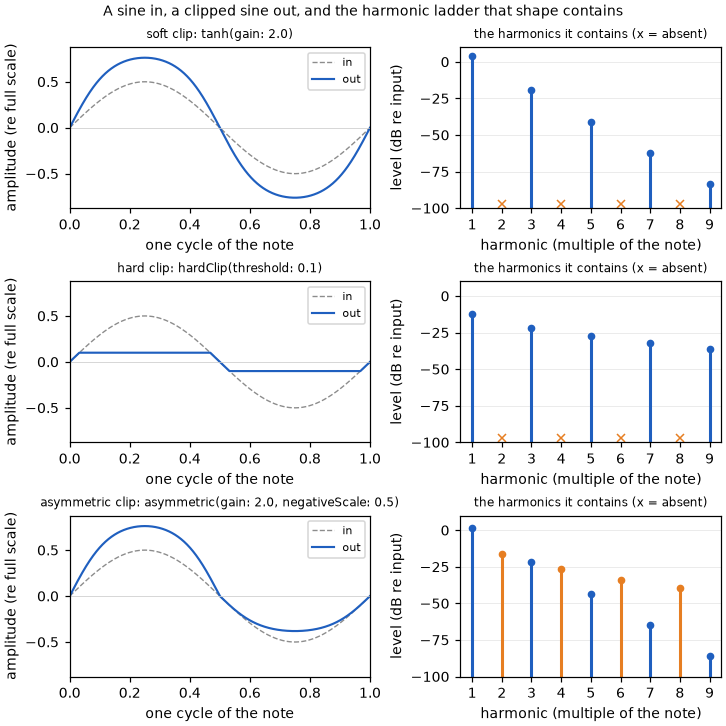
\includegraphics[width=0.95\linewidth]{explained-clipping.png}
  \caption{Three clippers, computed from their formulas at the amplitude
  the worked example uses (\hdAmplitude{} of full scale). Left: one cycle
  of a sine in (grey, dashed) and what comes out (blue). Right: the exact
  harmonic content of the output, in decibels relative to the input
  --- each step of 20 down is a tenth of the size. Odd harmonics in blue,
  even in orange; a cross marks a harmonic that is exactly absent.}
  \label{fig:clipping}
\end{figure}

The measurement, then, is a table: for each harmonic (the app reads
\hdHarmonicCount{} of them, the note itself and eight above it) and for
each note in the range, how loud that harmonic is compared with the note
that went in. It is drawn as one curve per harmonic across the notes ---
the \term{harmonic-response} --- with a single-number summary, the
\term{thd}, beside it. Everything is measured relative to the strength of
the test tone (\term{input-normalized}), so a plain wire reads as
``0~dB'' for the note itself and nothing for any harmonic, and two
measurements made at the same drive on different rigs can be laid over
each other.

\paragraph{What it cannot tell you.} Stated once, so nothing below has
to hedge.
\begin{enumerate}
  \item \textbf{Only one loudness.} One sweep is one drive level. A pedal
  that cleans up when you play softly, or hardens when you dig in, does
  so at other loudnesses this measurement never visits; the Gain Map and
  the Compression measurements own that axis.
  \item \textbf{Only one note at a time.} Two notes played together make
  the pedal produce sums and differences of their frequencies as well as
  harmonics. That is a different measurement --- Chord IMD --- and
  nothing here predicts it.
  \item \textbf{A number can be hiss, not harmonic.} The analysis reads
  whatever lands in each harmonic's slot, and the pedal's own noise lands
  there too. A separate check (\term{shaping}, below) says whether a
  reading is something the circuit did or just its noise; a reading is
  not automatically a harmonic.
  \item \textbf{Nothing below the rig's own floor.} The interface, the
  cables and the converters have noise and distortion of their own. Below
  that level the app is measuring the rig, and it says so rather than
  quoting a figure (\term{floor}, below).
  \item \textbf{Nothing about listening.} The chart says how much of each
  harmonic there is. It says nothing about what the distortion sounds like.
\end{enumerate}

\subsection{The test signal}

The test tone is a single sine that glides smoothly from a low pitch to a
high one --- from \hdStartHz{}~Hz to \hdEndHz{}~Hz over about
\hdRequestedDurationS{} seconds in the standard plan --- the
\term{sweep}. One signal visits every note in the range, so one recording
holds the answer for the whole neck. Figure~\ref{fig:sweep} shows its
first quarter second and how its pitch climbs over the whole sweep: the
pitch rises by the same musical interval in each second, which is why it
draws as a straight line on the pitch axis of the lower panel. The
\term{instantaneous-frequency} is the pitch the tone is at, at any given
moment.

\begin{figure}[htbp]
  \centering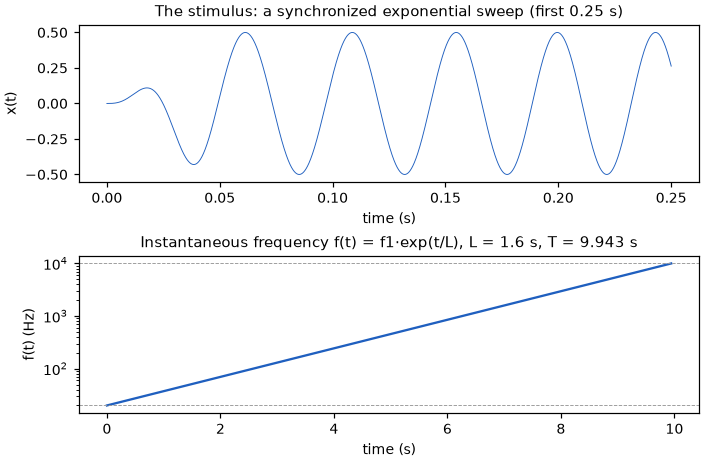
\includegraphics[width=0.9\linewidth]{hd-sweep.png}
  \caption{The test tone: its first quarter second (top) and its pitch
  over the whole sweep (bottom).}
  \label{fig:sweep}
\end{figure}

The speed of the glide is not free to choose. The trick that makes the
whole measurement possible is this: when a pedal clips a gliding tone, the
second harmonic it produces is itself a gliding tone, at twice the pitch
--- which is to say, it is a copy of the test tone that is running ahead
of it by a fixed amount of time. The third harmonic is another copy,
further ahead; the fourth further still. For those copies to line up
exactly, the tone's climb has to be timed so that it completes a whole
number of cycles before each copy's head start --- the
\term{synchronization}, met by nudging the requested length
slightly (the standard plan's \hdRequestedDurationS{}-second request
becomes \hdActualDurationS{}~s; its \term{rate-constant} is
\hdRateConstantS{}~s). The nudge is what lets each harmonic be pulled out
afterwards as its own clean copy. In the standard plan the second harmonic
runs \hdDelayTwoS{}~s ahead of the note, the third \hdDelayThreeS{}~s and
the ninth \hdDelayNineS{}~s.

The first and last moments of the tone are faded in and out rather than
switched, so nothing bangs. During those fades the pedal was driven by a
tone that was still rising or already falling, and a reading there
describes the fade, not the pedal. The range of notes the tone played at
full strength --- the \term{excited-band}, from \hdExcitedBottomHz{}~Hz to
\hdExcitedTopHz{}~Hz in the standard plan --- is where every number in
the chapter is meant.

\subsection{How the answer is pulled apart}

The recording that comes back from the pedal is a gliding tone with its
harmonics riding on it, all overlapping in time. Separating them takes
three steps.

\paragraph{Undoing the glide.} The first step is \term{deconvolution}:
applying the exact mathematical undo of the test tone --- its
\term{inverse-filter}, written down from the tone's formula rather than
measured --- to the recording. Undoing a glide turns it into a single
sharp blip at one instant. Because every harmonic is a copy of the tone
running a known amount ahead, each harmonic turns into its own blip, that
same amount earlier in time. The result, the \term{impulse-response}, is
shown in Figure~\ref{fig:deconvolved}: the note itself is the blip at
zero, and the harmonics stand in a row to its left, each at its own head
start. Each one is a \term{harmonic-pulse}. The example is a symmetric
soft clipper, so only the odd harmonics have blips; at the even positions
there is nothing, as there should be.

\begin{figure}[htbp]
  \centering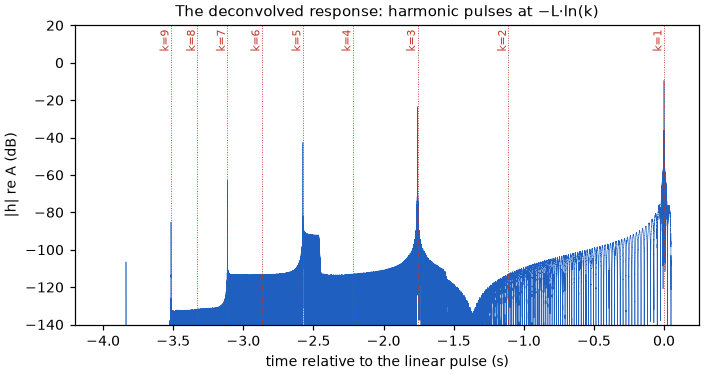
\includegraphics[width=0.95\linewidth]{hd-deconvolved.png}
  \caption{The recording after the glide is undone, for the worked
  example (a symmetric soft clipper). The note is the blip at time zero;
  each harmonic is a blip that much earlier. The even positions are empty
  because the clipper is symmetric.}
  \label{fig:deconvolved}
\end{figure}

\paragraph{Cutting each blip out.} The second step cuts each harmonic's
blip out of that row with an \term{extraction-window}: a slice of time
centred on the blip, tapered smoothly to nothing at both ends so that the
cut itself adds no edges. Each slice is as wide as it can be without
reaching into the neighbouring blip, up to a cap of \hdWindowCapS{}~s on
either side --- so the note and the first few harmonics get the full
\hdWindowFullS{}~s, and higher harmonics, whose blips crowd closer
together, get less (the ninth gets \hdWindowNineS{}~s).
Figure~\ref{fig:windows} shows the nine slices over their blips. A wider
slice can tell finer pitch differences apart, so the high harmonics are
read a little more coarsely than the low ones. If a sweep is so short that
a slice would shrink below \hdMinimumHalfWidthSamples{} samples on either
side, that harmonic and every one above it is not reported at all: a
short sweep simply carries fewer harmonics.

\begin{figure}[htbp]
  \centering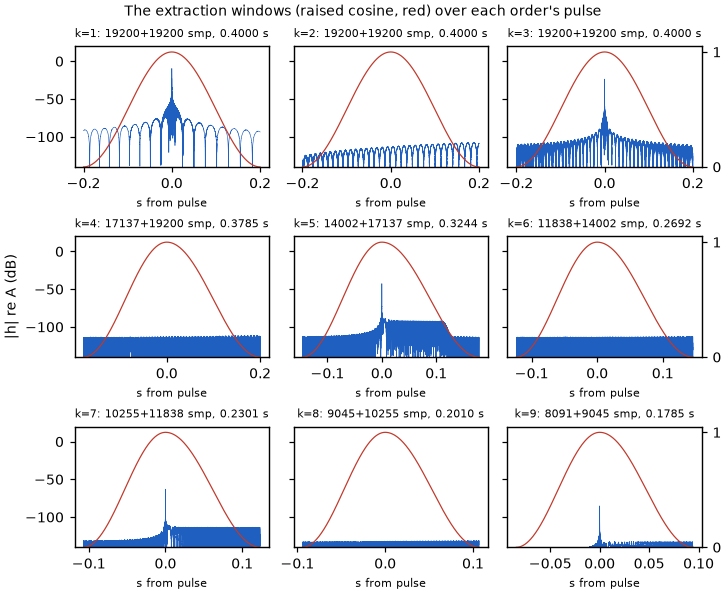
\includegraphics[width=0.95\linewidth]{hd-windows.png}
  \caption{The nine slices (red) over their blips (blue). The first three
  take the full width; from the fourth on, the gap to the next blip sets
  the width.}
  \label{fig:windows}
\end{figure}

\paragraph{Reading a harmonic at a note.} Each slice, once cut out,
holds one harmonic's behaviour across every note at once. The app turns it
back into a curve against frequency, and reads the harmonic for the note
you care about at that harmonic's own frequency: the third harmonic of a
note is read at three times the note's frequency, the ninth at nine
times. (The curves are drawn against the note you play, but each point on
the ninth-harmonic curve was read nine times higher up.)

\paragraph{Where a reading stops being honest.} A digital recording
cannot hold a tone above half its sample rate; anything higher folds back
down to a lower frequency instead of vanishing (an \term{alias-image}).
For a high enough note, the tenth harmonic --- which the pedal produces
whether or not the app reads it --- folds back onto exactly the frequency
where the ninth is being read, and from that note upward the ninth
harmonic's reading is contaminated. Every harmonic has such a note, and
the higher the harmonic, the lower the note at which its next neighbour
lands on it. That note is the harmonic's \term{validity-bound}, and past
it the app draws the curve faded and uses none of the values. In the
standard plan at \hdSampleRateHz{}~Hz, the ninth harmonic is readable up
to \hdTopNoteNineHz{}~Hz (around \hdTopNoteNineName), the fifth up to
\hdTopNoteFiveHz{}~Hz --- all far above the top of a guitar's range, so
for the notes you actually play every harmonic is inside its bound.

\begin{center}
\hdPlainWindows
\end{center}

\subsection{THD, in one sentence}

The \term{thd} figure adds up everything the pedal added at multiples of
the note --- every harmonic from the second up that lies inside the
audible band (\hdAudibleLowHz{}~Hz to \hdAudibleHighHz{}~Hz) and inside
its validity bound --- and divides the total by the note itself, so that
``ten percent'' means the added harmonics together are a tenth the size
of the note. It is a proportion of the note, not a verdict, and it is
computed the same way at any sample rate because the audible band is
fixed. It is THD and not THD+N: noise is deliberately not in the sum,
which is why the checks in the next section matter --- a harmonic slot
that holds only hiss would otherwise count as distortion. Toward the top
of the neck the sum loses its harmonics one at a time as each leaves the
audible band or its validity bound; from the first note where that
happens the app draws the curve broken, because it is then counting fewer
harmonics, not measuring less distortion. The curve is sampled at
\hdThdGridPoints{} notes from \hdThdGridLowHz{}~Hz upward (the very
lowest notes are fade-in territory and are skipped).

\subsection{Three checks the app makes before it believes a number}

\paragraph{The floor.} Every rig has a \term{floor}: a level below which
what the app reads is the interface's own noise and distortion, not the
pedal's. The app measures it during calibration, with a cable in place of
the pedal, and reads it against every harmonic at every note. A reading
that sits at or below the floor is reported as a bound --- ``at most this
much'' --- never as a figure, because nothing quieter than the rig can be
seen through the rig. The floor is not one number: it depends on the
note, on how loud the sweep was played, and on how many sweeps were
averaged (playing the sweep \hdDefaultAverages{} times back to back and
combining the results, the app's default, lowers the noise part of the
floor by about \hdAveragingFourDB{}~dB; eight sweeps by about
\hdAveragingEightDB{}~dB). That lowering applies only where what the rig
contributes is noise; at the faded ends of the sweep, where the residue
is the measurement's own, averaging buys nothing and the floor stays put.

\paragraph{Fundamental presence.} The THD figure, and everything else
that compares a harmonic with the note, divides by the note. A few
devices --- an octave-up fuzz turned all the way up, a ring modulator ---
remove so much of the note that what comes back at the note's frequency
is no longer the pedal but the analysis machinery's own leakage. The app
has measured how far below the loudest harmonic a reading of the note can
sit before that happens --- \hdSeparationDB{}~dB, established on devices
whose answers were known in advance --- and where a record crosses that
line it stops quoting anything that divides by the note
(\term{fundamental-presence}). The harmonic levels themselves are still
real and are still shown; the ratio to a note that is not there is not.

\paragraph{Shaping: circuit or hiss?} The analysis reads whatever landed
in each harmonic's slice, and the pedal's own hiss lands there too. For a
symmetric clipper the even harmonics are exactly absent, so what the app
reads at the even positions \emph{is} its hiss --- often well above the
rig's floor, and still not distortion. The \term{shaping} check separates
the two by looking at how a harmonic's reading behaves across
neighbouring frequencies. Something a circuit did varies smoothly and
consistently from one frequency to the next; noise does not --- its
readings scatter, each one unrelated to its neighbours. The app computes
a \term{coherence} score for that orderliness over \hdShapingWindowSamples{}
neighbouring readings (pure noise scores about \hdUnshapedCoherence{}
on it, a perfectly orderly response scores 1), converts the score into
how far the reading stands above the noise in it, and calls the reading
\emph{shaped} only when that margin is at least \hdShapedSNRDB{}~dB. With
the score comes a \term{scatter}: how far a single reading might be off
purely because of the noise in it, stated in dB alongside the level (a
reading that is pure noise carries about \hdUnshapedScatterDB{}~dB of
it). A reading that fails the check is drawn dotted and faded, the legend
says ``at the floor --- noise, not a response'', and nothing downstream
--- the THD sum, the comparison distance, the summaries --- treats it as
a harmonic.

\paragraph{Averaging, since it came up.} When the sweep is played more
than once, each repeat is analysed on its own and then the repeats are
combined. Before combining, each repeat is lined up with the first to a
fraction of a sample (\term{derotation}) --- a timing drift of even a
fraction of a sample between repeats would otherwise blur the high
harmonics into looking politer than they are. The combination is of the
full readings, direction included, never of the levels alone: averaging
levels would make a biased number more precise, not more right. This is
\term{averaging}; the app offers \hdOfferedAverages{} sweeps and defaults
to \hdDefaultAverages, with a \hdGapS{}~s gap between repeats.

\subsection{What the result looks like}

Figure~\ref{fig:magnitude} is the worked example --- a symmetric soft
clipper whose exact answer is known --- as the pipeline reads it. Each
solid curve is one harmonic's measured level across the notes, in dB
relative to the input; the dashed line under each is the exact answer,
which the solid curve sits on. Where a curve turns dotted it has passed
its validity bound, and the shaded strip at the far right is the fade-out,
where the last point reads the fade rather than the device. The even
harmonics are not drawn at all: for a symmetric clipper they are exactly
absent, and the pipeline reads nothing there but the arithmetic's own
dust, far below the chart. The note itself reads above zero because this
clipper also adds gain.

\begin{figure}[htbp]
  \centering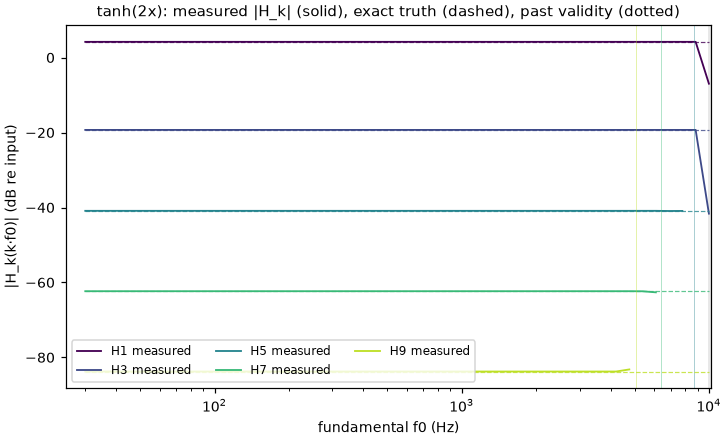
\includegraphics[width=0.95\linewidth]{hd-magnitude.png}
  \caption{The worked example: measured level of each odd harmonic
  (solid) against the exact answer (dashed) across every note. Dotted
  segments lie past the harmonic's validity bound; the shaded strip is the
  fade-out.}
  \label{fig:magnitude}
\end{figure}

The two charts the app draws for a real record are shown next, rendered
from the app's own chart code on its simulated pedal (never a screenshot).
The first is the Harmonic Distortion chart itself. Each curve is one
harmonic; the legend names it and says what it is musically --- the
second harmonic is an octave up, the third an octave and a fifth, and so
on --- with the odd family in one colour and the even family in another,
so the symmetry rule from the first section can be read straight off the
chart. The horizontal axis is the note you play, labelled with note names
and their frequencies; the vertical axis is the harmonic's level in dB
relative to the input, and its label says how the axis was scaled. The
shaded band marks a guitar's range. Where a curve fades and breaks near
the top it has crossed its validity bound. The lines under the chart
state the drive level the sweep was played at and, for a real capture,
how many sweeps were averaged --- read them before comparing two records,
because a harmonic level only means something at a stated loudness.

\begin{figure}[htbp]
  \centering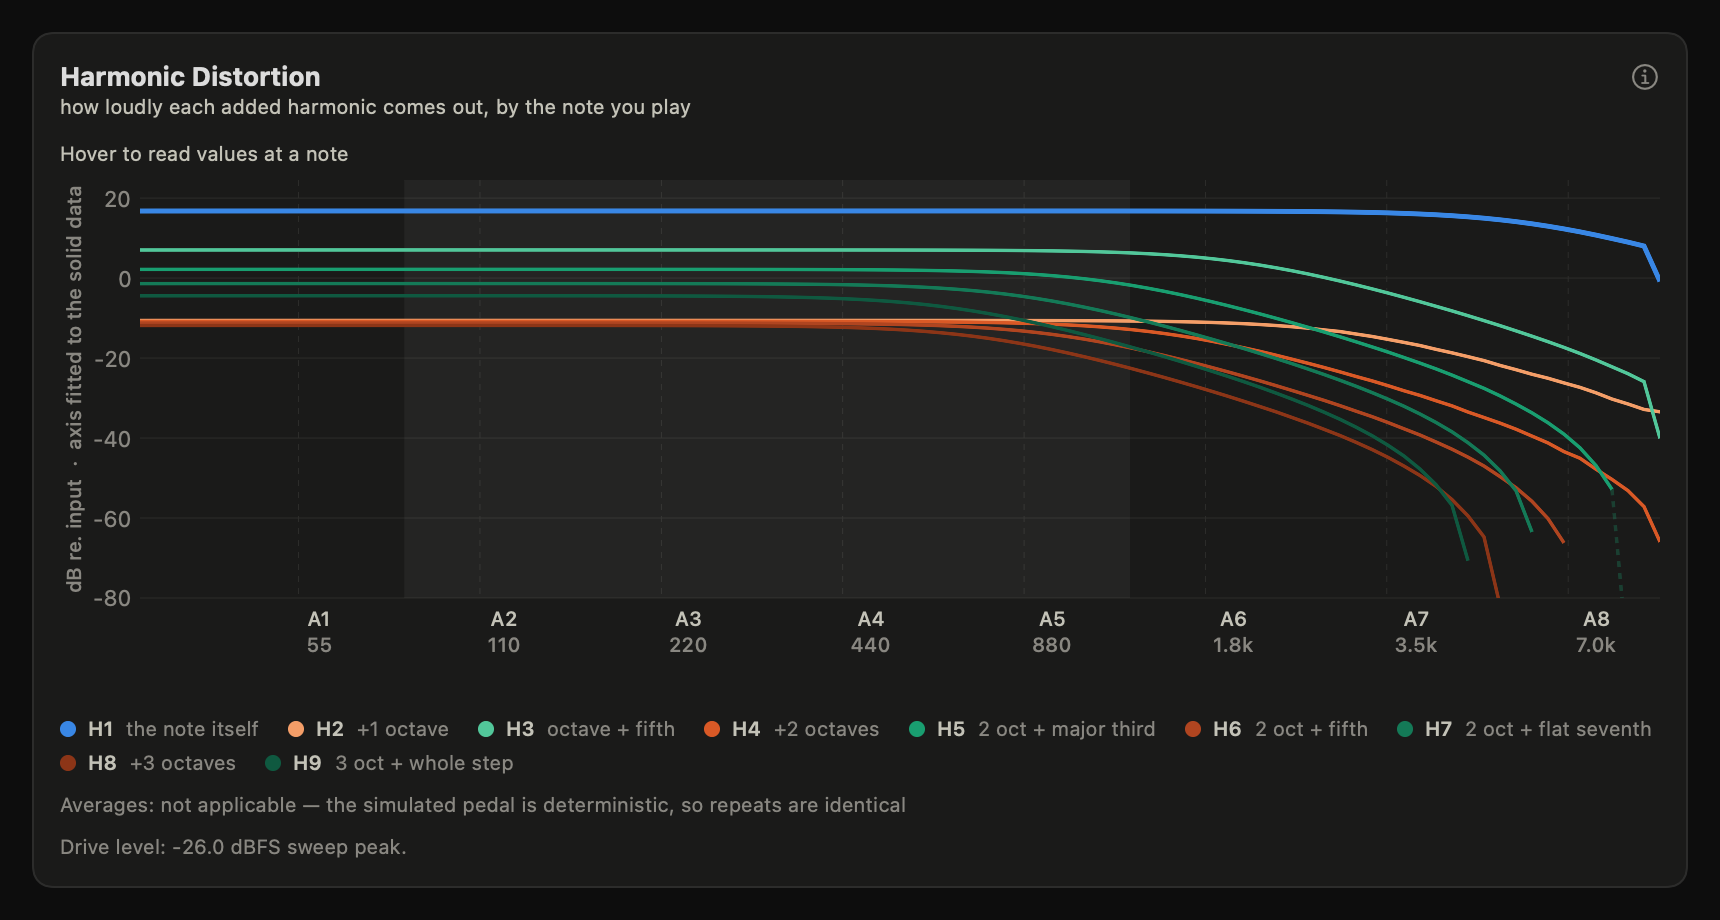
\includegraphics[width=0.85\linewidth]{harmonic-distortion--sim.png}
  \caption{The Harmonic Distortion chart as the app draws it, for its
  simulated pedal.}
\end{figure}

The second chart is Distortion vs.\ Note: the THD figure, in percent,
across the same notes. A flat curve means the pedal adds the same
proportion of harmonics at every note; a curve that falls toward the top
of the neck usually means the pedal's own tone filter is shaving the
harmonics off. Where the curve turns dashed, the sum has begun losing
harmonics to the band edge, one at a time, and the line under the chart
names the note at which each one left --- from there the curve falls
because it counts fewer harmonics, not because the pedal cleaned up. The
vertical axis is fitted to the notes before that point, so the dashed tail
may run off the bottom of the chart; that is the honest picture of a sum
with fewer terms in it.

\begin{figure}[htbp]
  \centering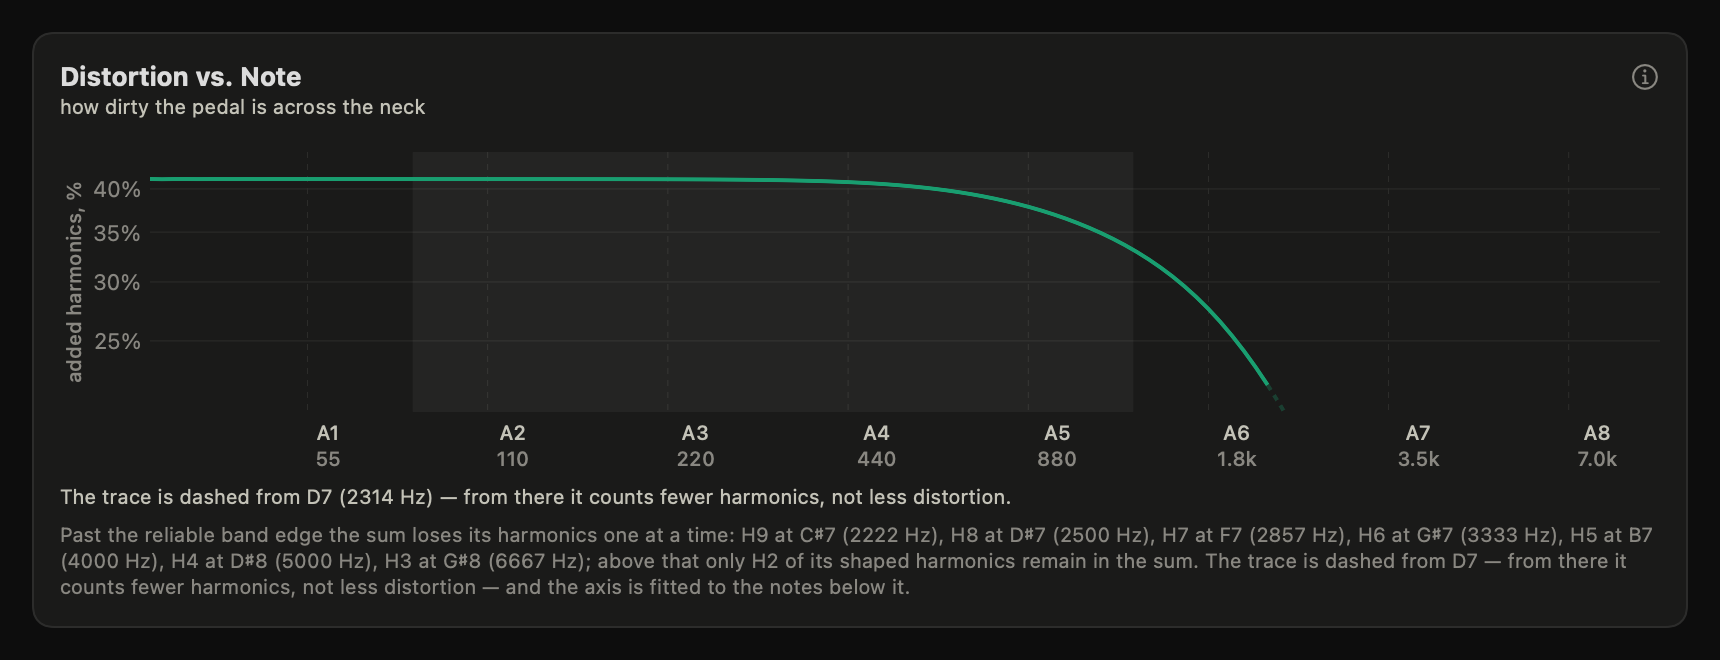
\includegraphics[width=0.85\linewidth]{harmonic-distortion--sim-thd.png}
  \caption{The Distortion vs.\ Note chart as the app draws it, for the
  same simulated pedal.}
\end{figure}

\subsection{How you can check that the app does what this says}

Everything above is a description, and a description can drift from the
code it describes. The pipeline behind these documents guards against
that in a way anyone can rerun. The app's own measurement code writes out
the \term{manifest}: every setting that determines a result, obtained by
calling the code that owns it. From that manifest and the published
method, a second program was written --- in Python, independently, not by
translating the app's code --- and the \term{parity} runs both on the
same made-up devices and demands the same answer.

The made-up devices are the point. Three of them are formulas --- the
soft clipper of the worked example, a hard clipper and a gentle
polynomial curve --- whose exact harmonic content can be computed on
paper, so both programs are held not only to each other but to the truth.
The fourth is a \term{phantom}: a recording built to contain exactly a
chosen set of harmonics and nothing else, so the analysis is asked to
read back precisely what was put in.

The demands, in numbers the pipeline writes into this document: the two
programs must agree to within \paritySwiftToleranceWords{} of a decibel
(\paritySwiftTolerance{}~dB) at every harmonic and every note (on the run
that built this document the worst disagreement was
\parityWorstSwiftWords{} of a decibel, \parityWorstSwift{}~dB --- the two
differ only in the last digits of floating-point arithmetic); on the
phantom, both must be
within \parityAliasFreeTolerance{}~dB of the exact answer over the whole
range; on the formula devices, within stated tolerances
(\parityPerSampleTolerances) over the lower half of each harmonic's range
--- the upper half is where a computed device, unlike a real pedal
through a real interface, folds harmonics from above the sample rate
back into the band, and that folding is the device's, not the method's.
For the worked example the exact answer is \parityTanhHone{}~dB for the
note itself, \parityTanhHthree{}~dB for the third harmonic and
\parityTanhHnine{}~dB for the ninth, and both programs read them back
within those tolerances. A fifth case adds noise and averages four
sweeps, and requires every reading the shaping check calls shaped to sit
within \parityScatterMultiple{} times its own stated scatter of the
truth --- the check on the check.

The test runs automatically on every change to the app, and the tables
and figures in both documents are regenerated on every change and
compared with the committed copies: a method change that the description
does not follow is a failing build, not a stale page. The scripts, the
test and the instructions for running them are in the repository named
on the first page.

\subsection{Where it stops being a measurement}

\begin{itemize}
  \item \textbf{The faded ends.} The very first and very last moments of
  the sweep are ramps, and a reading there is a reading of the ramp.
  Numbers from those notes describe the measurement, not the pedal; the
  app excludes them where it can and draws them faded where it cannot.
  \item \textbf{A loud harmonic leaks a little into its neighbours'
  slices.} How much is measured, not assumed, and the app never claims a
  harmonic deeper below the loudest one than that leakage allows. Where
  the note itself is that far down, the fundamental-presence check
  withdraws every ratio to it.
  \item \textbf{A number can be noise.} A harmonic slice that holds only
  hiss still yields a number. The shaping check is there to say so, and a
  reading it rejects must not be read as a harmonic, however confidently
  it is drawn.
  \item \textbf{The simulated pedal folds its own harmonics.} The app's
  virtual pedal applies its clipping to the signal sample by sample, so
  the harmonics it makes above half the sample rate fold back into the
  band --- an error a real pedal through a real interface does not carry.
  The user guide's Simulation Mode page states it; the parity numbers
  above measure it, and it is largest in each harmonic's top
  half-octave.
  \item \textbf{Short sweeps carry fewer harmonics.} Each harmonic needs
  a slice at least \hdMinimumHalfWidthSamples{} samples wide on each side
  of its blip; a sweep much shorter than the standard plan runs out of
  room for the high ones, and they are simply not reported.
  \item \textbf{The range's top point.} The THD curve asks for
  \hdThdGridRequested{} notes and can deliver \hdThdGridPoints{}: its
  topmost point lands a hair above the sweep's end and is dropped rather
  than read under the fade.
\end{itemize}

\clearpage

\section{Transfer Curve}
\label{sec:transfer-plain}

\subsection{What this measurement tells you, and what it cannot}

The Harmonic Distortion chapter inferred a pedal's clipping from the
harmonics it adds. This measurement draws the clipping itself. The app
plays one steady low note into the pedal, records what comes back, and
plots the output against the input, moment by moment, over one cycle of
the note: the \term{transfer-curve}. A plain wire draws a straight
diagonal line --- what comes out equals what went in. A clipper draws a
line that bends over at the top and the bottom, and the bends are its
clipping shape, seen directly rather than deduced.

\paragraph{Reading a picture of output against input.} Each instant of
the recording is one dot: how far across is the input at that instant,
how far up is the output. As the note swings up and down, the dot travels
out to the right, back through the middle, out to the left and back
again, and over a whole cycle it traces a path. If the pedal's output
depends only on the input at that same instant --- the same input always
gives the same output, whether the wave is on its way up or on its way
down --- the outward and return journeys land on the same path, and the
picture is a single line. Figure~\ref{fig:transfer-cycle} shows the
worked example, a soft clipper with no filter, both ways: the path as the
app sees it on the left, and the same input and output cycles laid out
against time on the right. The path retraces itself exactly, so the line
is the device's clipping formula, and the exact formula drawn over it
cannot be told apart from it.

\begin{figure}[htbp]
  \centering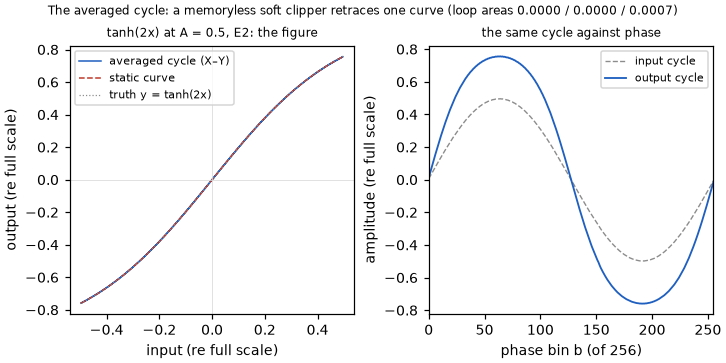
\includegraphics[width=0.95\linewidth]{transfer-cycle.png}
  \caption{The worked example, a soft clipper with no filter, at the
  loudest hardware drive and the standard note. Left: the averaged cycle
  as the app plots it, output against input, with the app's static curve
  (dashed) and the exact formula (dotted) over it --- the three coincide.
  Right: the same input and output cycles against position in the cycle.
  The title gives the three loop areas, all zero to the resolution of the
  slots.}
  \label{fig:transfer-cycle}
\end{figure}

\paragraph{Why a time shift draws a loop.} Now suppose the output is an
undistorted copy of the input that arrives a little late. At any moment
the output is what the input was a moment ago, so the same input value
now meets two different outputs --- one on the way up, another on the way
down --- and the outward and return journeys separate: the path opens
into an oval. Figure~\ref{fig:ellipse} builds one. On the left, a sine
and a shifted copy of itself; in the middle, the oval the two draw when
one is plotted against the other; on the right, what the worked example's
clipper followed by the same shift draws --- the bends are the clipper,
the opening is the shift. How fat the oval is depends on the size of the
shift as a fraction of the cycle: no shift is a line, a quarter of a
cycle is a circle. A shift like this is what every tone filter does,
because a filter passes each frequency with its own small delay, so a
pedal with any tone shaping in it draws an oval even when it adds no
distortion at all.

\begin{figure}[htbp]
  \centering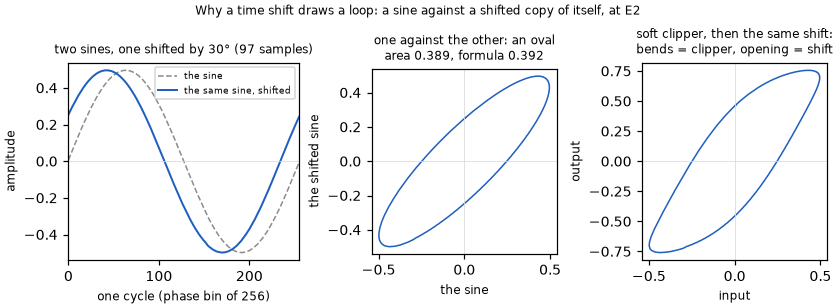
\includegraphics[width=0.98\linewidth]{explained-ellipse.png}
  \caption{Left: a sine and the same sine shifted in time by a twelfth of
  a cycle. Middle: the oval the pair draws when one is plotted against the
  other, with its area as a fraction of the box and the value the formula
  for a pure shift predicts. Right: the worked example's soft clipper
  followed by the same shift --- the bends are the clipper and the opening
  is the shift.}
  \label{fig:ellipse}
\end{figure}

\paragraph{The word ``memory''.} There is a second way to open the loop,
and it is the one this measurement is really after. If the circuit's
output depends not only on the input now but on where the signal has just
been --- a bias point that drifts with the signal, charge stored in a
capacitor that leaks back out over the next few cycles --- then the same
input value again meets different outputs on the way up and on the way
down, and the path opens. That is memory, and its loop looks like the
filter's oval. Telling the two apart is the whole difficulty of this
chapter, and the phase removal below is the app's answer.

The measurement's result is the averaged cycle itself, the line through
the middle of it, and three loop areas, each stated as a fraction of the
picture's box: the total, the part a tone filter's shift accounts for, and
the part left over.

\paragraph{What it cannot tell you.} Stated once.
\begin{enumerate}
  \item \textbf{Only one loudness.} One note at one drive is one operating
  point. A pedal whose clipping starts above that drive draws a straight
  line --- not clean, merely not driven into its bends. The Gain Map and
  the Compression measurements visit other loudnesses.
  \item \textbf{Whether an open loop is memory or a tone filter.} Ordinary
  tone filters open the loop with no memory in the circuit. The phase
  removal exists to take the filter's part out, and even then the middle
  band of loop sizes is reported with a hedge, for a reason the next
  section gives.
  \item \textbf{The clip levels of a lopsided clipper.} Every pedal has a
  capacitor on its output that removes the wave's average level. It
  centres a clipper that clips the top harder than the bottom, so the two
  clip levels come out equal in the picture even when the circuit's are
  not; the lopsided shape survives as even harmonics in the Harmonic
  Distortion measurement instead (the limits section).
  \item \textbf{The rig's own timing error.} If the recording is lined up
  with the test tone a fraction of a sample late, the picture opens into
  an oval the measurement cannot tell from the device's own --- and it is
  a property of the rig, not of the pedal (the limits section).
  \item \textbf{Nothing about listening.} The picture shows the clipping
  shape. It says nothing about what the distortion sounds like.
\end{enumerate}

\subsection{The test signal}

The test tone is a single sine at one note, held steady. The standard
note is \tcNote{} (\tcNoteHz{}~Hz, the low E string), and the standard
loudness is \tcLevelDBFSRounded{}~\term{dbfs}, the same drive the
Harmonic Distortion sweep uses, so that the two measurements describe the
pedal at one operating point. The tone lasts \tcDurationS{}~s --- about
\tcTotalCycles{} cycles of the note --- with \tcPrerollS{}~s of silence
before it and \tcTailS{}~s after, and its first and last \tcFadeMs{}~ms
are faded rather than switched, so nothing bangs. The first
\tcSkipCycles{} cycles (about \tcSkippedS{}~s) are left out of the
analysis while the circuit settles into the tone; everything from there to
the end of the tone is used. The app measures the delay through the rig
on every capture and lines the recording up with the tone before anything
below happens.

The app offers \tcProbeNoteCount{} probe notes (\tcProbeNotes) and a
note-range capture at \tcRangeNotes; the drive can be set from
\tcFloorDBFS{} to \tcCeilingDBFS{}~dBFS on hardware (a plugin can be
driven to \tcPluginCeilingDBFS{}~dBFS, digital full scale). The worked
example throughout this chapter uses the loudest hardware drive,
\tcCeilingDBFS{}~dBFS --- an amplitude of \tcCeilingAmplitude{} of full
scale --- because at the standard drive the reference clippers the method
is checked against barely bend at all. That is the point of the level
control: this measurement shows the shape only where the note reaches it.

\subsection{How the picture is built}

Seven steps, each in words; the technical reference gives each one as an
equation.

\paragraph{Folding the cycles together.} The recording holds about
\tcBinnedCycles{} usable cycles of the note. Each cycle is divided into
\tcBins{} equal slots by position within the cycle, every sample goes into
its slot, and each slot's samples are averaged --- the input's and the
output's separately. That gives one \term{averaged-cycle}: \tcBins{} input
values and \tcBins{} output values, one pair per slot. Noise, which is
different in every cycle, averages toward nothing; the shape, which
repeats, stays. The right-hand panel of Figure~\ref{fig:transfer-cycle}
is that cycle, and the left-hand panel is the same \tcBins{} pairs plotted
against each other. Every sample from the skipped opening to the end of
the tone is folded in, the closing fade included --- the limits section
returns to that.

\paragraph{The box.} Loop areas need a scale, or a loud signal's loop
would read larger than a quiet one's for no reason. Every area is divided
by the area of the rectangle the whole picture fits inside, the
\term{box-normalization}, so that an area is a fraction: a loop filling
the whole box would read one, and a line reads zero.

\paragraph{Counting the area lobe by lobe.} A loop can cross itself. A
figure-eight is two lobes traced in opposite directions, and the textbook
way of measuring an enclosed area, which keeps track of direction, would
let the two cancel and report nothing. The app instead cuts the path at
every crossing and adds up the size of every lobe regardless of which way
it was traced: the \term{lobe-area}. A lobe smaller than \tcLobeFloor{} of
its own box is dropped as the jitter of the averaging.

\paragraph{The oval a tone filter draws.} The best-fitting oval is drawn
through the loop using only the note itself --- the fundamental of each of
the two cycles, nothing above it. That oval is the
\term{fundamental-ellipse}, and its area is exactly what a shift of the
note in time would draw: the linear part of the loop, a filter's doing,
never memory. Figure~\ref{fig:decomposition} shows the worked example's
clipper behind a tone filter (a high-pass just below the guitar's range):
the raw loop, the oval fitted to it, and what remains.

\paragraph{What is left.} The oval's output is subtracted from the output
cycle, and the loop that remains is measured the same way, lobe by lobe:
the \term{nonlinear-loop-area}, the headline memory figure. It is the
harmonics' own loop. In a clipper with no memory and no filter the
harmonics keep step with the note and retrace; a harmonic that has been
shifted --- by a filter, or by memory --- encloses area here.

\begin{figure}[htbp]
  \centering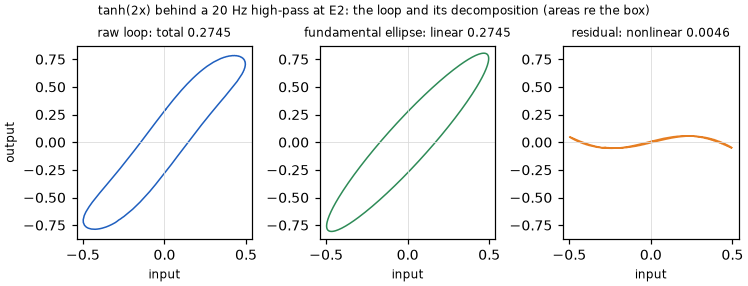
\includegraphics[width=0.95\linewidth]{transfer-loop-decomposition.png}
  \caption{The worked example's soft clipper behind a 20~Hz high-pass at
  the standard note: the raw loop (left), the oval fitted to its
  fundamental (middle), and what is left once the oval's output is
  subtracted (right), each titled with its area as a fraction of the box.
  The filter draws the oval; what is left is small.}
  \label{fig:decomposition}
\end{figure}

\paragraph{The line through the middle.} The \term{static-curve} is the
app's estimate of the clipping shape with the loop ignored. The cycle is
cut at the input's lowest and highest points into a rising pass and a
falling pass; each pass is resampled onto the same \tcStaticGrid{} evenly
spaced input values, and the two are averaged. It is done pass by pass,
rather than by sorting every sample by its input value, because a sine
spends most of its time near its peaks and hardly any near zero ---
sorting by input value would starve the middle of the curve.

\paragraph{The memory verdict.} The \term{memory-verdict} is the app's
three-way call on the nonlinear loop area (of the corrected picture, when
the phase removal has been applied): under \tcMemorylessBelowPct{}~percent
of the box the device reads memoryless-ish, from \tcMemoryFromPct{}~percent
it reads memory, and between the two the reading is hedged, deliberately.
The reason is a tone filter placed \emph{ahead} of the clipper. Such a
filter shifts the note before it is clipped, and the harmonics the clipper
then makes are shifted along with it --- the second harmonic by twice the
note's shift, the third by three times --- so the harmonics no longer keep
step with the note, and they enclose area with no memory in the circuit at
all. From a single note the app cannot tell that from mild memory, and it
says so instead of choosing.

Every one of these quantities is recomputed from the stored cycle each
time a record is read; the record keeps the cycle and nothing that a later
fix would have to migrate.

\subsection{Three things the app checks before it believes the picture}

All three lean on the pedal's paired Harmonic Distortion record --- the
sweep measurement of the previous chapter, of the same pedal at the same
setting --- when one exists. Nothing they decide is stored; each is
re-decided from the two records every time.

\paragraph{The right way up.} A plugin is measured inside the computer,
and its recording is lined up with the test tone by finding the best
match --- which, for a steady tone, can land exactly half a cycle off. The
picture then comes out upside down, and for a lopsided clipper worse than
that: each input is paired with the output from half a cycle later. The
\term{orientation} check reads where the note sits in the captured cycle.
When it sits within \tcLockToleranceDeg{}~degrees of exactly in step or
exactly reversed, the alignment is known to have locked to the tone; if
the pedal's polarity (next) then disagrees with the way the picture is
drawn, the output cycle is moved on by half a period and the picture
redrawn. In every other case the picture is shown as captured and nothing
is implied. A hardware capture is lined up by a different method that
keeps the pedal's true timing, and is immune.

\paragraph{Polarity.} \term{polarity} is whether the pedal turns the wave
upside down. It is read from the paired record, over the low notes: does
the note come back the same way up or inverted, with the louder readings
counting for more. The confidence is how consistently the answer comes
out, on a scale where one is perfect agreement, and the reading counts as
confident only above \tcPolarityThreshold{}. A device that shifts the note
by a quarter of a cycle is neither one nor the other; it reads as not
confident rather than as a guess.

\paragraph{Is the note there?} The memory verdict, the polarity statement
and the pairing check below all depend on the note itself being in the
recording. A few devices remove it (an octave-up effect, a ring
modulator), and what is then read at the note's frequency is the
analysis's own leakage. The app takes the \term{fundamental-presence}
reading from the paired record, which separates the note from its
harmonics far better than one averaged cycle can (the
\tcSeparationDB{}~dB bound of the previous chapter), and where the note
is absent it draws the raw picture and states none of the three.

\paragraph{The phase removal.} This is the longest part of the chapter,
and the part a reader most needs.

\emph{The problem.} A tone filter shifts each frequency in time by its
own amount. A filter \emph{after} the clipper shifts each harmonic by the
filter's own delay at that harmonic's frequency. A filter \emph{before}
the clipper shifts the note, and the clipper's harmonics inherit multiples
of that shift --- two, three, four times it. The two cases look alike in
the picture and are corrected differently, and the obvious repair
(correct each harmonic by the filter's delay at that harmonic's frequency)
is wrong exactly when the filter sits before the clipper --- which is
where a pedal's tone control usually sits.

\emph{What the paired record knows.} The sweep measurement read each
harmonic at its own frequency as the pedal made it, filters before and
after included. So the paired record already holds every harmonic's true
timing, whichever side of the clipper the filters sit on. The
\term{phase-removal} rests on that: the picture's harmonic timings are
compared with the paired record's, and the difference is what the
filters did to the picture.

\emph{Lining the two recordings up.} The two measurements were made
separately and each measured its own delay through the rig, so a small
time offset between them is legitimate, and it has to be found before
anything else --- treated as a filter shift, it would be ``removed''
wrongly. The \term{frame-fit} finds the one offset that makes every
harmonic agree at once, louder harmonics counting for more, by scanning
every offset within half a cycle. Whatever disagreement remains after
that, over the harmonics above the note, is the \term{pairing-residual}:
the test of whether the two records really describe one device at one
setting. Above \tcResidualToleranceRad{} radians
(\tcResidualToleranceDeg{}~degrees of a cycle) the app declines.

\emph{Who votes.} A harmonic takes part only when both records hold it
clearly --- at least \tcMagnitudeFloorDB{}~dB relative to the note on each
side --- and it is inside its validity bound in the paired record. Fewer
than \tcMinimumTerms{} voting harmonics is too little evidence, and the
app says so rather than fitting through what it has.

\emph{The two allowed positions, and the fold.} In a pedal with no memory
and no filtering, every harmonic sits in one of two positions relative to
the note: exactly in step with it, or exactly reversed. Which of the two
is the device's own doing --- a clipper's third harmonic is reversed ---
and the picture keeps it. That pair of positions is the \term{lattice},
and a measured harmonic's distance from the nearer of its two positions is
what the filters added. But ``nearer'' is ambiguous once a filter has
shifted a harmonic more than a quarter of the way round, so the app folds
in order. The note itself goes first, anchored by the polarity: inverting
means reversed; without a confident polarity the nearest position is
taken, and the sign is then quoted only within a stated confidence. Each
higher harmonic is folded against a prediction made from the ones already
folded --- a straight ramp with the harmonic number, which is the shape a
filter before the clipper produces, plus the paired record's own
low-frequency shape, which is the filter after it. The working assumption
is that what a harmonic carries beyond that ramp is under a quarter turn:
true of the resistor-and-capacitor networks pedals are built from, and
weakest at the lowest harmonic, where it has held on every device class
measured.

\emph{The correction.} Once each harmonic's added shift is known, the
whole picture is re-timed: a smooth correction across every frequency in
the cycle that moves each one in time and makes none louder or quieter.
It is measured up to the highest harmonic that voted --- the support, that
harmonic's number times the note --- and extended smoothly above it, and
the app's caption states the support and that the correction is
extrapolated above it. Figure~\ref{fig:compensation} is the case the
obvious repair cannot handle: the soft clipper behind a filter placed
before it. The raw picture is a wide loop with the clipping bends on it;
the corrected picture is the clipper's own curve, laid over the exact
memoryless answer.

\begin{figure}[htbp]
  \centering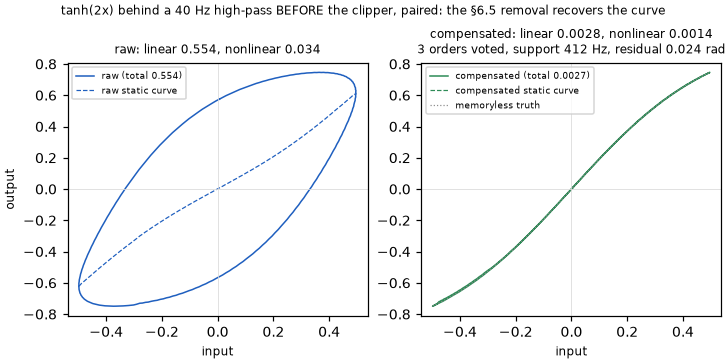
\includegraphics[width=0.95\linewidth]{transfer-compensation.png}
  \caption{The soft clipper behind a 40~Hz high-pass placed before the
  clipper, paired with its own sweep measurement. Left: the raw loop and
  its static curve. Right: the corrected picture over the exact memoryless
  curve, with how many harmonics voted, the support and the residual.}
  \label{fig:compensation}
\end{figure}

\emph{Five outcomes.} Corrected; a pairing mismatch, when no offset
reconciles the harmonics; too little evidence, when fewer than
\tcMinimumTerms{} harmonics vote; a negligible loop, when the raw total is
under \tcDeadZonePct{}~percent of the box --- there is nothing to correct,
and this outranks a mismatch, so a tiny noise-dominated loop never wears a
warning (the fit still runs, so polarity can still be stated); and a
tripped guard, when a correction that passed the residual nonetheless grew
one of the loop areas by more than \tcMetricGuardTolerance{} of the box
over the raw picture, in which case the raw picture stands. A pairing
mismatch has two possible causes the residual cannot separate: the two
records come from different settings or sessions, which measuring both
again together resolves; or the device is one whose harmonics have no
fixed timing relationship to the note (a frequency doubler), which no
re-measurement resolves. The app names the class, not the cause.

\emph{Polarity, stated.} The picture states the pedal's polarity only when
the fit ran, its residual confirmed the pairing, and the note's position
resolved; otherwise the tile stays empty. Absence is honest; a guessed
sign is not.

\subsection{The settings}

Every setting is in the technical reference's Transfer Curve chapter, in
a table read from the manifest; this chapter repeats only the handful a
reader acts on. The standard note is \tcNote{} at \tcNoteHz{}~Hz and the
standard loudness \tcLevelDBFS{}~dBFS (an amplitude of \tcAmplitude{} of
full scale); the tone lasts \tcDurationS{}~s at \tcSampleRateHz{}~Hz, so
one cycle is about \tcSamplesPerCycle{} samples; the first \tcSkipCycles{}
cycles are skipped; the cycle is folded into \tcBins{} slots and the
static curve is drawn on \tcStaticGrid{} input values; the memory
verdict's two thresholds are \tcMemorylessBelow{} and \tcMemoryFrom{} of
the box; and the phase removal declines above a residual of
\tcResidualToleranceRad{} radians, needs \tcMinimumTerms{} voting
harmonics, and does nothing at all when the raw loop is under
\tcDeadZone{} of the box.

\subsection{What the result looks like}

Figure~\ref{fig:transfer-cycle} is the pipeline's own rendering of the
worked example. On the left, the averaged cycle plotted output against
input, with the static curve and the exact formula over it; the three
coincide, which is what a memoryless device with no filter looks like
here. On the right, the same input and output cycles side by side against
position in the cycle: the output is the input with its peaks pushed in
and rounded --- the clipping --- and taller, because this clipper also
adds gain. The title gives the three loop areas, all zero to the
resolution of the slots.

The app's own chart, rendered from its chart code on its simulated pedal
(never a screenshot), is Figure~\ref{fig:app-transfer}. Four tiles run
across the top: the drive note and its frequency; the memory figure ---
the nonlinear loop area, with the verdict's word under it; the linear
phase loop --- the oval's area, labelled as filter phase and not memory;
and the polarity, with a plain-words gloss. Under the chart's title, the
lines state whether the phase removal was applied, through how many of
the measured harmonics it was fitted, up to what frequency the correction
is measured (extrapolated above), which record it was removed against,
and the alignment residual in radians. The chart itself draws the loop in
blue and the static curve dashed in orange, labelled as both directions
averaged; what goes in runs across, what comes out runs up. For the
simulated pedal the loop is closed and the two lines coincide. On a real
pedal with an open loop, the dashed line is the app's estimate of the
clipping shape through the middle of it, and the limits section says
where that estimate is weakest.

\begin{figure}[htbp]
  \centering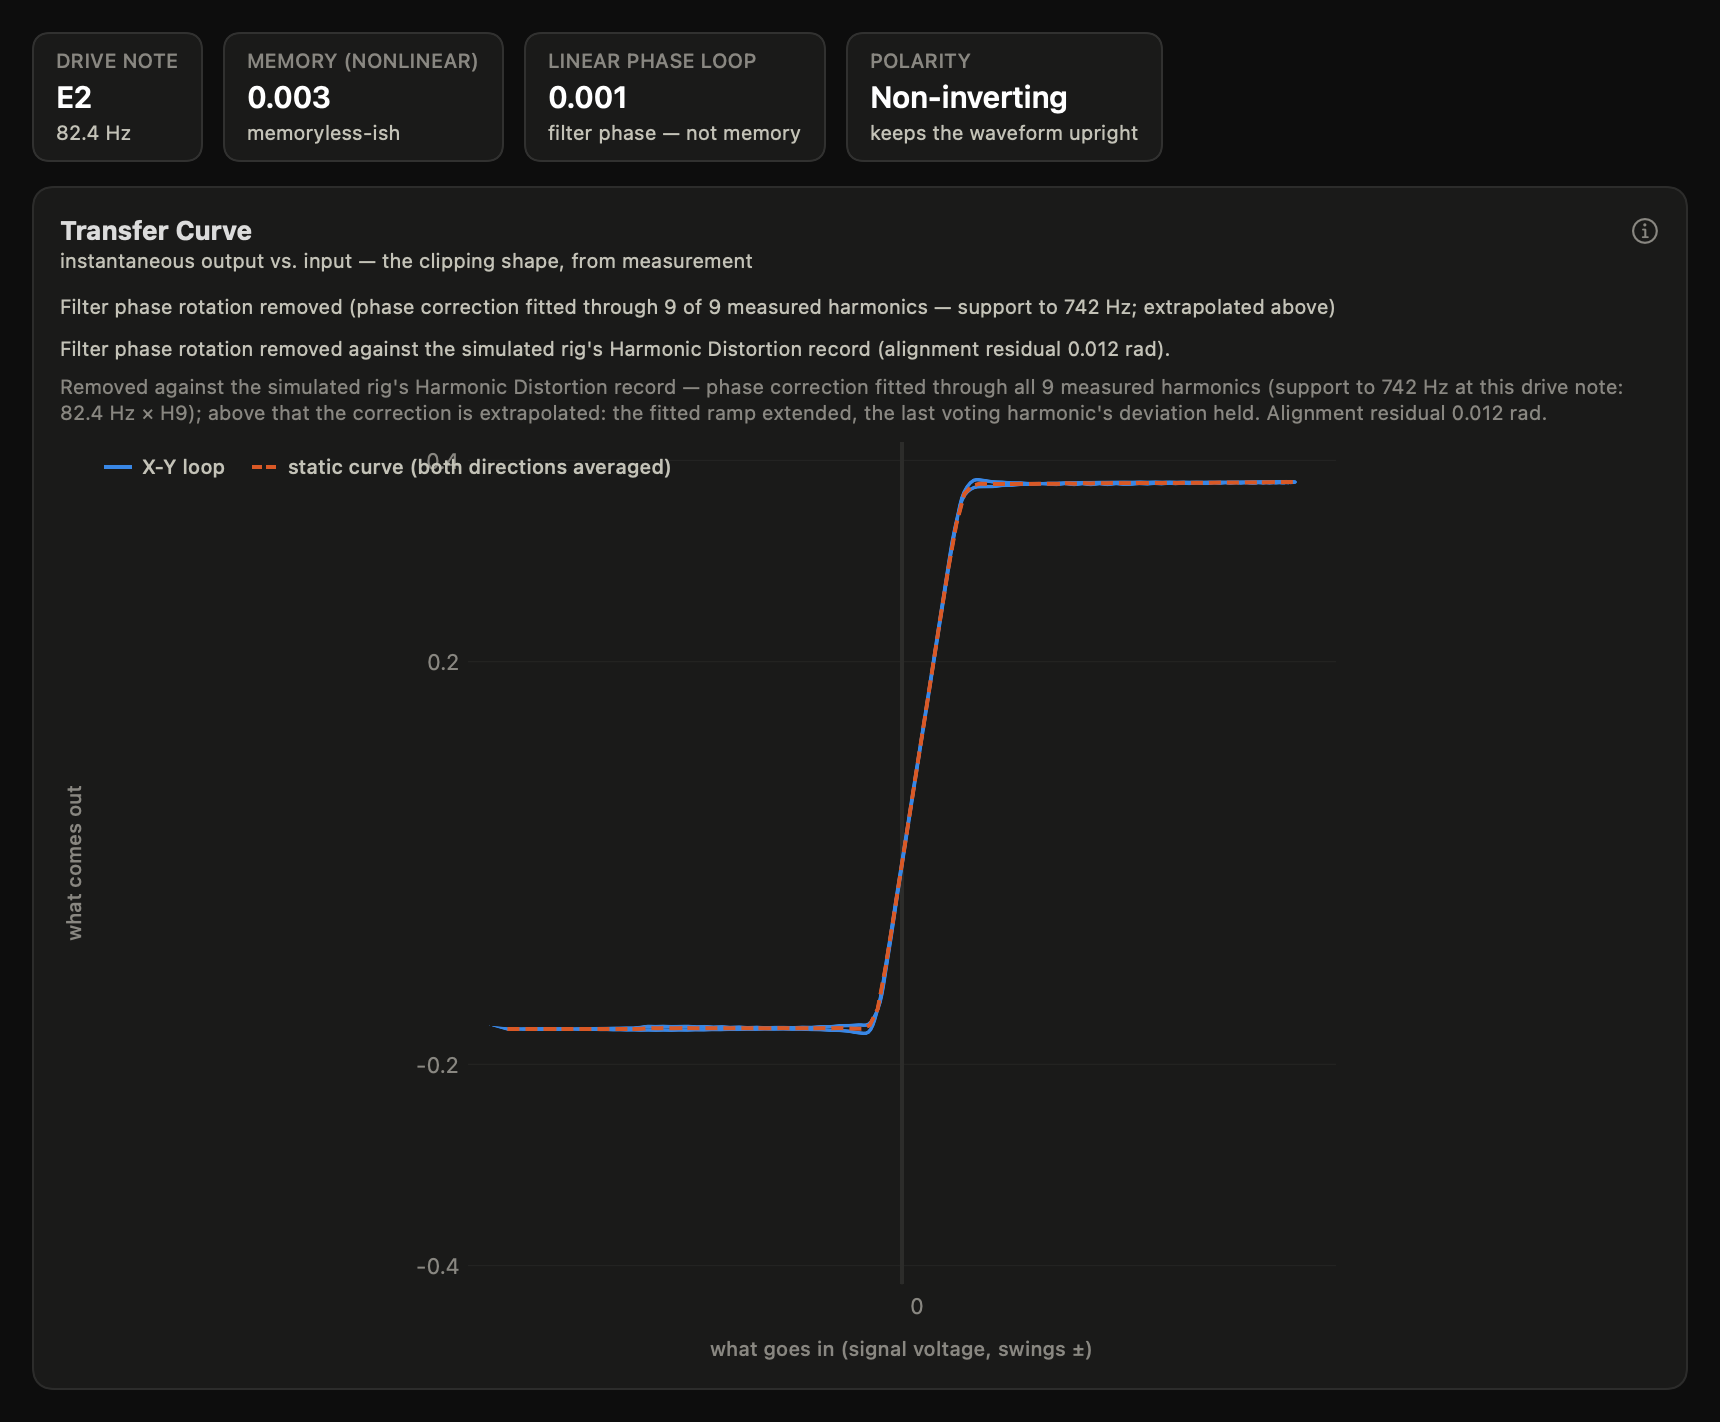
\includegraphics[width=0.85\linewidth]{transfer-curve--sim-compensated.png}
  \caption{The Transfer Curve view as the app draws it, for its simulated
  pedal, with the phase removal applied.}
  \label{fig:app-transfer}
\end{figure}

\subsection{How you can check that the app does what this says}

As in the previous chapter, a second program was written from the
description --- in Python, independently, not by translating the app's
code --- and the \term{parity} runs both on the same made-up devices
and demands the same answer. Here the made-up devices come in three
kinds. Memoryless clippers with no filter, whose exact curve is their
formula, so the picture can be checked against the truth point by point.
Linear devices --- a wire behind a tone filter, and a wire read with a
deliberately planted timing error --- whose oval must match the formula
for a pure shift. And filtered clippers, with the filter after the clipper
or before it, measured by the sweep of the previous chapter as well so
that the phase removal can be run and its answer checked against the
memoryless truth. That last kind is the one that matters: the removal is
held not only to the app but to what the clipper would have drawn with no
filter at all. In total the test runs \tparityCaseCount{} cases.

The demands, in numbers the pipeline writes into this document. The two
programs must agree on every value in the cycle, on the static curve, on
the corrected picture, on every area and on every fitted quantity to
within \tparitySwiftWords{} (\tparitySwift; on the run that built this
document the worst disagreement was \tparityWorstSwiftWords,
\tparityWorstSwift, the last digits of floating-point arithmetic), and
must find the same time offset to within \tparitySwiftShiftWords{} of a
sample (the measured difference was \tparityWorstShift); every yes-or-no reading --- the
outcome class, the flip, the polarity, the verdict, the presence --- must
be identical. The oval drawn for a linear device must match the formula
for a pure shift to within \tparityEllipseRatioWords{} at the plan's tone
length (measured: at worst \tparityEllipseDeficitShort~percent short) and
to within \tparityEllipseRatioLongWords{} when the tone is ten times
longer (measured \tparityEllipseDeficitLong~percent) --- the limits
section says why the length matters. On a smooth clipper the raw static
curve must sit within \tparityRawStaticSmoothWords{} of the output peak of
the exact curve (measured \tparityTanhStaticWords, \tparityTanhStatic); on
a hard clipper within \tparityRawStaticHardclipWords{} (measured
\tparityHardclipStaticWords, \tparityHardclipStatic, because
\tcBins{} slots round a sharp corner); and a memoryless device's nonlinear
loop area must stay under \tparityMemorylessNonlinearWords{} of the box
(measured \tparityWorstMemorylessNonlinearWords,
\tparityWorstMemorylessNonlinear). Every paired filtered device must come
out corrected on both sides, with the planted time offset found to within
\tparityFrameShiftWords{} of a sample (measured
\tparityWorstFrameShiftWords, \tparityWorstFrameShift), a residual under
\tparityResidual{} radians (measured \tparityWorstResidual; the app's own
accept bar is \tcResidualToleranceRad), the memoryless curve recovered to
within \tparityCompStaticWords{} of peak (measured
\tparityWorstCompStaticWords, \tparityWorstCompStatic), and both corrected
loop areas under \tparityCompAreaWords{} of the box (measured
\tparityWorstCompAreaWords, \tparityWorstCompArea). \tparityRemovalStatus

Two of those results are worth stating in words. The clipper behind a
filter placed before it has no memory at all, and its raw nonlinear loop
area reads \tparityPrehpRawNonlinear{} --- inside the memory verdict's
hedged band; the removal takes it to \tparityPrehpCompNonlinear{}. The
hedge in the pipeline section is exactly this case. And the half-cycle
lock is undone: on the case built to land half a cycle off, the note's
captured position read \tparityShiftPsi{} radians, a half turn to within
\tparityShiftLatticeDistanceWords{} of a radian, the paired polarity read
non-inverting, and the resolved picture rises from left to right.

The test runs automatically on every change to the app, and the tables
and figures in both documents are regenerated on every change and
compared with the committed copies; the scripts and the instructions for
running them are in the repository named on the first page.

\subsection{Where it stops being a measurement}

\begin{itemize}
  \item \textbf{The oval's formula is for a linear device only.} The rule
  that turns a shift into an oval's area assumes the device's peak is the
  note's own. A clipped output's peak is not, so on a clipper the oval's
  area can read larger than that rule gives. A reader who wants the shift
  as an angle should apply the rule to a linear-device measurement only,
  and the pipeline's own check reads the rule to
  \tparityEllipseDeficitShort~percent at the plan's tone length and
  \tparityEllipseDeficitLong~percent at ten times it --- so a deficit of
  several percent on a hardware capture is in the measurement chain, not
  in the rule.
  \item \textbf{The closing fade is folded in.} The skipped opening cycles
  protect the start of the tone; the last \tcFadeMs{}~ms ride their fade
  into the averaged cycle. Their share of the average shrinks with the
  tone's length, which is the whole of the deficit above: it is why the
  pipeline checks the oval at ten times the tone length as well, where
  the share is gone.
  \item \textbf{A leftover timing error is a loop.} Any timing error left
  between the tone and the recording --- the app removes a whole number
  of samples, and the fraction of a sample at least stays --- shifts the
  note by an amount that grows with the note's frequency, and draws an
  oval on a plain wire (Figure~\ref{fig:delay}). On a pedal that
  \term{alignment-error} loop cannot be told from the pedal's own filter
  loop. A reader can test it: measure two notes on one rig, and a single
  timing error must account for both ovals. The nonlinear loop area is
  untouched by it on a linear device.
  \item \textbf{The output capacitor hides unequal clip levels, not
  unequal harmonics.} A clipper that clamps at different heights carries
  an average level, and the \term{coupling-capacitor} every pedal has on
  its output strips it, leaving equal heights from an unequal circuit
  (Figure~\ref{fig:coupling}). The shape asymmetry remains, and the even
  harmonics in the paired sweep measurement are where it is read. Because
  every pedal has one, a transfer curve essentially never shows the raw
  asymmetry of an asymmetric clipper.
  \item \textbf{The correction is measured only as high as the last
  voting harmonic.} A harmonic too quiet to clear the floor on either
  side does not vote --- the soft clipper at this drive seats
  \tparityTanhVoted{} harmonics, the asymmetric clipper
  \tparityAsymVoted{} --- and above the support the correction is extended,
  not measured. A hard-clipped device has content far above it.
  \item \textbf{The paired timing is read at the nearest point.} The
  paired record's timing for a harmonic is read at the nearest frequency
  it holds, so a read can be off by up to half a step of that grid; the
  frame fit absorbs it as a spurious offset of a fraction of a sample
  (measured up to \tparityWorstFrameShift{} samples on the check cases)
  and leaves the rest in the higher harmonics' residuals.
  \item \textbf{The slots round a corner.} With \tcBins{} slots per cycle
  a hard clip's corner is averaged over one slot's width of input, and the
  static curve departs from the exact curve there by a few percent of the
  clip level; the smooth devices read under one percent of peak.
  \item \textbf{The line through an open loop is weakest at the ends.}
  The static curve averages the rising and falling passes, and the two
  meet at the input's extremes, which is where the estimate is least
  trustworthy; on a wide oval it departs from the true line by a few
  percent of peak there. The app draws it dashed, and that is the reason
  to read its ends with care.
  \item \textbf{A declined removal names its class, not its cause.} The
  residual separates a genuine pairing from a mismatch; it does not
  separate a session mismatch from a structural one, and the two need
  different remedies (the phase removal, above).
\end{itemize}

\begin{figure}[htbp]
  \centering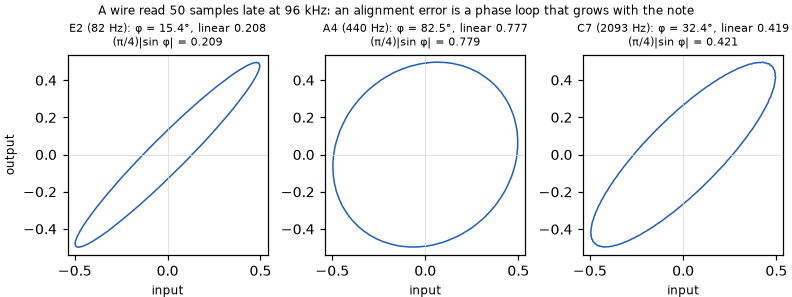
\includegraphics[width=0.95\linewidth]{transfer-delay-loop.png}
  \caption{A plain wire, read 50 samples late, at three notes: a timing
  error is a loop that grows with the note. Each title gives the shift the
  error amounts to at that note, the measured oval area and the value the
  formula for a pure shift gives.}
  \label{fig:delay}
\end{figure}

\begin{figure}[htbp]
  \centering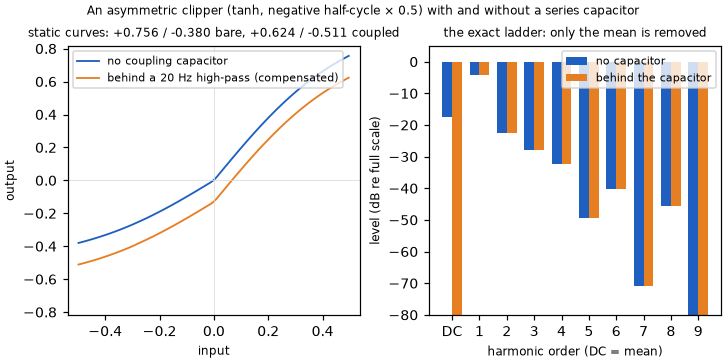
\includegraphics[width=0.95\linewidth]{transfer-coupling.png}
  \caption{A lopsided clipper (the bottom half scaled to one half) with
  and without a series capacitor at its output: the static curve's unequal
  clip levels are centred by the capacitor (left), while the exact
  harmonic ladder loses only its average level --- the even harmonics
  survive (right).}
  \label{fig:coupling}
\end{figure}

\clearpage
\section{Compression}
\label{sec:compression-plain}

\subsection{What this measurement tells you, and what it cannot}

The Harmonic Distortion measurement listed what a pedal adds to one note
at one loudness. This measurement keeps to one note --- one pitch, held
steady --- and changes the loudness instead: the note is played at every
rung of a ladder of loudnesses, quietest first, and at each rung the app
reads two things, how loud the note came out and how much distortion came
with it. The result is the \term{compression-curve}, the app's ``touch
response'': how much louder the output gets for each step louder at the
input.

\paragraph{A curve of output against input.} The picture the chapter
turns on is simple to draw and worth drawing once. Across the bottom is
how loud the note went in, up the side is how loud it came out, both in
\term{decibel}s, and each rung of the ladder is one dot. A pedal that
does nothing but pass the note draws a straight line at exactly one dB
out for every dB in --- \emph{one-for-one}, the line every panel in this
chapter draws dashed. A pedal with gain draws the same line higher up. A
pedal that compresses draws a line that starts one-for-one and then bends
over: past some loudness each step louder in produces less than a step
louder out, and at the extreme none at all. Figure~\ref{fig:ladder-plain}
is the whole idea in one picture, computed from a steep soft clipper (the
\term{tanh} curve of the earlier chapters with its input multiplied by
eight before the bend, as the panel titles print --- steeper because the
gentler one barely bends inside the ladder, a fact the section on reading
a record back returns to). On the left is the test note's loudness over
time: the ladder climbing, one rung marked. In the middle is that one rung
close up. On the right is the curve the rungs draw, with the two straight
lines the app fits through it and the corner where they meet. That corner
is the \term{knee}, and most of this chapter is about how it is found and
when it may be believed.

\begin{figure}[htbp]
  \centering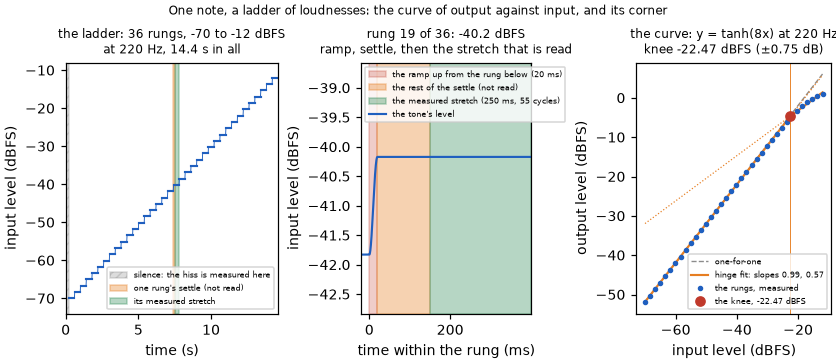
\includegraphics[width=0.98\linewidth]{explained-ladder.png}
  \caption{One note, a ladder of loudnesses. Left: the test note's level
  over time --- the silence before it, where the hiss is measured, then
  the rungs climbing, with one rung's settle (orange) and measured stretch
  (green) marked. Middle: that rung close up --- the short ramp from the
  rung below, the rest of the settle, then the stretch that is read.
  Right: output level against input level at the rungs for the steep soft
  clipper named in the title, the one-for-one line dashed, the two fitted
  lines of the hinge (dotted where each is extended past the corner) and
  the corner, which is the knee.}
  \label{fig:ladder-plain}
\end{figure}

When a record is opened, the app states three things beside the curve,
each worked out afresh from the stored rungs: the knee --- a loudness, or
``at or below'' a loudness when the test could not see it; the
\term{cleanup-reading} --- where, going up the ladder, the distortion
first crosses the line the chart draws, or that it never does, or that it
always is over it; and whether the note itself came through well enough
for any of that to be quoted. Each has its own part of the section on
reading a record back.

\paragraph{What it cannot tell you.} Stated once.
\begin{enumerate}
  \item \textbf{Only one note.} The curve is one pitch. A pedal with a
  tone control ahead of its clipper compresses differently at another
  pitch, and the Gain Map (Section~\ref{sec:journey-plain}) is where
  loudness meets pitch.
  \item \textbf{Nothing between two rungs.} The corner is placed by a fit
  through all the rungs and may land between two of them, but a feature
  narrower than a rung --- a straight dead region against a very steep
  soft onset --- looks the same when the whole of it falls between two
  rungs. The fine window below exists for that.
  \item \textbf{A knee the ladder did not reach.} A pedal already
  compressing at the quietest rung has its knee somewhere below it, and
  the honest answer is a bound --- ``at or below the quietest rung'' ---
  never a number.
  \item \textbf{A distortion reading near the hiss.} Toward the quiet end
  the note shrinks and the rig's hiss does not, so a distortion figure
  there can be the hiss. The hiss line described later says where, and
  each rung is labelled.
  \item \textbf{The second crossing.} The cleanup level is the first
  crossing from the quiet end. A pedal whose distortion rises, falls and
  rises again as it is driven harder --- some soft-knee overdrives do this
  --- is quoted at its first crossing only.
  \item \textbf{The last rung is read under the test's own fade.} The
  note fades out inside the last rung's measured stretch, so that rung
  reads a few thousandths of a decibel low; the limits section gives the
  figure.
  \item \textbf{The loudness axis is the signal, never a knob.} How loud
  the note goes in is how hard the circuit is driven, as your pick and
  your guitar's volume knob drive it. The pedal's own knobs are not
  touched while a curve is measured; to see what a knob does, you measure
  one curve per position.
  \item \textbf{Nothing about listening.} The curve says how the output's
  level and its distortion follow the input's level. It says nothing about what the distortion sounds like.
\end{enumerate}

\subsection{The test signal: a ladder of loudnesses}

The ladder first. On a hardware rig the note is played at
\cmpHardwareSteps{} rungs from \cmpHardwareFloorDBFS{} to
\cmpHardwareCeilingDBFS{}~\term{dbfs}, a span of \cmpHardwareTravelDB{}~dB
climbed in equal steps of \cmpHardwareStepDB{}~dB. Equal steps in decibels
are equal \emph{ratios}: each rung is the same proportion louder than the
one below, not the same amount. That is the \term{probe-grid}. Its top
rung is held back from full scale on purpose: an interface's input is set
so that the pedal's output cannot clip the converter at the loudest drive,
and with the input staged that way the top rung is the loudest drive that
cannot clip it. Its bottom rung sits far enough under the top that a
high-gain pedal's knee is reached rather than bounded --- the pedal's own
hiss, not the interface, is what limits it, and the gate below measures
exactly that. A plugin has no converter to protect, so its ladder runs to
the very top, from \cmpPluginFloorDBFS{} to \cmpPluginCeilingDBFS{}~dBFS
in \cmpPluginSteps{} rungs of \cmpPluginStepDB{}~dB. The quietest rung, the
loudest and the count are the user's to change for a run, and a record's
ladder is read from its own rungs, never assumed.

\paragraph{The fine window.} Where a feature is too narrow for rungs
\cmpHardwareStepDB{}~dB apart to show, the measure sheet adds a
\term{fine-window}: extra rungs \cmpFineStepDB{}~dB apart over a span you
choose, capped at \cmpFineCap{} of them, so that a wide span spreads its
extra rungs out rather than growing the run. The extra rungs are merged
into the ladder and the whole list sorted, so they interleave the ordinary
ones; a fine rung that lands on top of an ordinary one is dropped. Over a
span from \cmpFineExampleLowDBFS{} to \cmpFineExampleHighDBFS{}~dBFS the
hardware ladder delivers \cmpFineExampleDelivered{} rungs, the ordinary
\cmpHardwareSteps{} plus \cmpFineExampleAdded{}.

\paragraph{Within each rung.} The \term{stepped-tone} is one sine at the
probe note --- \cmpNoteHz{}~Hz, the \cmpNoteName{} an octave above the
open A string (the figures in this chapter are at \cmpSampleRateKHz{}~kHz;
a run uses its calibration's rate) --- whose loudness climbs the ladder
without a break in the wave: the same sine runs through the whole
test, only its size changes. Each rung has two parts, the
\term{settle-window}: first \cmpSettleMs{}~ms in which the tone ramps
smoothly up from the rung below over its first \cmpRampMs{}~ms and the
pedal is then left to settle at the new loudness, unread; then the
\cmpMeasureMs{}~ms that is actually measured. That measured stretch is
trimmed to a whole number of cycles of the note --- \cmpMeasureCycles{}
cycles at the probe note, never fewer than \cmpMinimumCycles{} --- the
\term{cycle-snap}, and the next section says what it buys. A rung is
therefore \cmpStepS{}~s, the hardware ladder's tone \cmpToneS{}~s, and the
middle panel of Figure~\ref{fig:ladder-plain} is one rung as it is
played. The tone's final moments fade to nothing over one ramp, and that
fade lies \emph{inside} the last rung's measured stretch --- the limits
section returns to it.

\paragraph{The silence before, and where the assembly lives.} A hardware
or plugin run plays \cmpPrerollS{}~s of silence before the tone and
\cmpTailS{}~s after it, \cmpStimulusS{}~s in all. The silence before is
not padding: the app measures the loudness of whatever comes back during
it --- the loop's hiss and the pedal's own, in the same recording --- and
keeps that figure with the record as the \term{noise-stamp}. Everything
below that says ``the hiss'' means that number. The technical reference
notes that this arrangement --- the silence, the tone, the stamp, and the
delay the recording is cut by --- is assembled by the app's measurement
service rather than by a single shared function, and that Simulation Mode
assembles it differently (no silence, no stamp, a shorter settle); the
last section says what that costs.

\subsection{How the curve is built}

Five steps, each in words; the technical reference gives the exact rule
for each.

\paragraph{Cutting the recording to size.} Every signal through a rig
comes back a little late --- the round trip through the converters and
cables. The calibration measured that delay, and each rung's measured
stretch is cut out of the recording that much later than it was played,
after the silence before the tone. A plugin measures its own delay on
every render and hands back a recording with none, so its cut is the
silence alone. The delay is never guessed. A rung whose stretch would run
past the end of the recording is left out.

\paragraph{Asking for one exact pitch.} Each cut stretch is read for the
note and for its overtones by the \term{one-bin-estimator}, which does one
thing: it asks how much of exactly one pitch the stretch contains. The
cycle snap is what makes that question clean. A stretch that holds a
whole number of cycles of the note also holds a whole number of cycles of
every one of its overtones, so each of them fits the stretch exactly, and
a pitch that fits exactly is read at its full size while every other
pitch that fits exactly adds up to nothing --- the note's own presence
does not spill into the reading of its second overtone, or its third. The
stretch's two ends are tapered smoothly to nothing before the reading is
taken, which costs almost nothing on a pitch that fits and makes the
reading forgiving of the two things the snap cannot promise: the tail of
the ramp from the rung below, and a cut that lands a sample off. The
check at the end of the chapter measures both. (The Chord IMD measurement
reads a whole spectrum the same way, one slot per pitch, and
Section~\ref{sec:slots-plain} explains slots in general; here only a
handful of pitches are ever asked for.)

\paragraph{The gate.} Before a rung is read, its measured stretch's
overall level is compared with the hiss. A rung within
\cmpGateDB{}~dB of the hiss --- about \cmpGateRatioWords{} its size --- is
left out of the curve and counted: the \term{noise-gate}. Its ``output
level'' would be the hiss and not the note, and a run of such rungs at
the quiet end would draw as a flat line, which is what a compressed pedal
looks like. The quietest rung that survives is then the bottom of the
curve, and any bound reads from there. The record says how many rungs
were dropped.

\paragraph{The note and its overtones.} For each surviving rung the
estimator reads the note itself --- the \term{fundamental}, whose size is
the rung's output level --- and up to \cmpHarmonicsSummed{} overtones
above it, each \term{harmonic-order} in turn, stopping at the first that
would lie above the audible band (\cmpBandLowHz{} to
\cmpBandHighHz{}~Hz) or too close to half the sample rate; at the probe
note every rate the app offers reads all \cmpHarmonicsSummed{}, and only
above about \cmpBandTopNoteHz{}~Hz (\cmpBandTopNoteName) does the band's
top begin to take the highest away. The rung's \term{thd} is the size of
those overtones together, compared with the note --- the same figure as
chapter one's, THD and not THD+N: the hiss is deliberately not in the
sum, which is why the hiss line described later is needed.

\paragraph{What is stored, and what is not.} The rungs are sorted by
input level (a fine window's rungs interleave the ordinary ones) and the
record keeps the note, the sample rate, each rung's input level, output
level and distortion, the noise stamp and the dropped count. Nothing
described in the next section is stored: the knee, the cleanup reading
and every label are worked out afresh each time the record is opened, so
a better rule corrects every curve ever measured.

\begin{figure}[htbp]
  \centering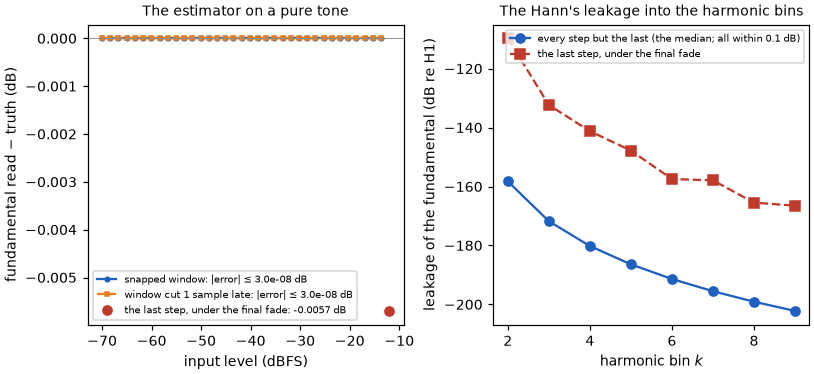
\includegraphics[width=0.95\linewidth]{compression-estimator.png}
  \caption{The estimator on a pure tone with nothing else in it. Left:
  how far its reading of the note sits from the truth at every rung, on
  the stretch cut exactly and on a stretch cut one sample late --- both at
  the arithmetic's own rounding --- and the last rung, which holds the
  final fade. Right: how much of the note leaks into the reading of each
  overtone, by overtone, on the cut stretch and under the fade.}
  \label{fig:estimator-plain}
\end{figure}

\subsection{What the app decides when it reads a record back}

Everything in this section is computed from the stored rungs every time a
record is opened.

\paragraph{The knee.} Between each pair of neighbouring rungs the app
takes the \term{incremental-slope}: how many dB louder the output got for
that step louder in. One dB out for a dB in is clean; no dB out for a dB
in is a wall. Those slopes are
the local picture; the knee comes from a fit through the whole curve. The
\term{hinge-fit} draws the curve as two straight lines joined at a
corner, and slides the corner along the input axis --- through
\cmpCandidates{} candidate positions between the second rung and the
third from the top, so that each line keeps at least two rungs --- solving
for the best pair of lines at each position and keeping the corner where
the two lines miss the rungs least. Against that stands the plainest
alternative: one straight line through everything. The right-hand panel
of Figure~\ref{fig:ladder-plain} shows the fit on the worked example.

\emph{Two kinds of answer.} The corner is reported as a \emph{number}
only when the quiet end of the curve is clean, in a stated sense, and
otherwise as a \emph{bound}. The app decides in a fixed order.
\begin{enumerate}
  \item If bending the line does not cut the miss to \cmpNoBreakWords{} of
  the single line's or less --- if the bend buys almost nothing --- the
  curve is one line. A line at \cmpUnityGuardWords{} of one-for-one or
  steeper is no knee at all: the pedal is clean throughout. A shallower line is a
  pedal compressing mildly everywhere, and its knee is ``at or below the
  quietest rung''.
  \item If the corner's upper line still climbs at \cmpSlopeThresholdWords{}
  of one-for-one or more, the pedal does not compress in this range: no
  knee.
  \item The \term{unity-guard}: if the lower line is shallower than
  \cmpUnityGuardWords{} of one-for-one, no clean stretch anchors the
  fit. The pedal was already compressing at the quietest rung, the corner
  the fit found is an artifact of a curve bent everywhere, and the answer
  is a bound at the quietest rung, with the fitted slope quoted beside it
  as the evidence. The test is against one-for-one and not against the
  compression threshold of the previous step, and the difference matters:
  every slope between the two is a pedal that is compressing, gently, at
  its quietest rung, and the guard used to let those through as confident
  numbers.
  \item The \term{bound-zone}: a corner within one rung of the bottom of
  the ladder cannot be anchored from below --- it might lie lower still
  --- and is a bound at that position.
\end{enumerate}
Otherwise the corner is a number, with a \term{resolution-band}: the
range of corner positions that fit the rungs within
\cmpResolutionBandPercent{}\,\% of the best. Half that range is the knee's
resolution, never finer than the spacing between candidate positions, and
it sets the decimals the level is shown with --- a tenth of a decibel when
the resolution is \cmpDecimalsBarDB{}~dB or better, a whole decibel when it
is not. A bound's resolution is the ladder's own step, because nothing
finer is knowable there, and its label reads ``$\le$''.
Figure~\ref{fig:knee-plain} shows the two cases as the fit sees them: for
each candidate corner, how badly the two lines miss the rungs. A hard
clipper whose threshold lies inside the ladder makes a sharp dip with a
narrow band around it, and the corner is a number. The same clipper with
its threshold below the quietest rung makes a curve that falls toward the
bottom with no dip to trust, and the verdict is a bound at the quietest
rung by the unity guard. And ``no knee'' is a real answer, not a failure:
the soft clipper of the earlier chapters at its gentler setting bends so
little inside the hardware ladder that no corner is found, which is why
this chapter's worked example is the steeper one.

\begin{figure}[htbp]
  \centering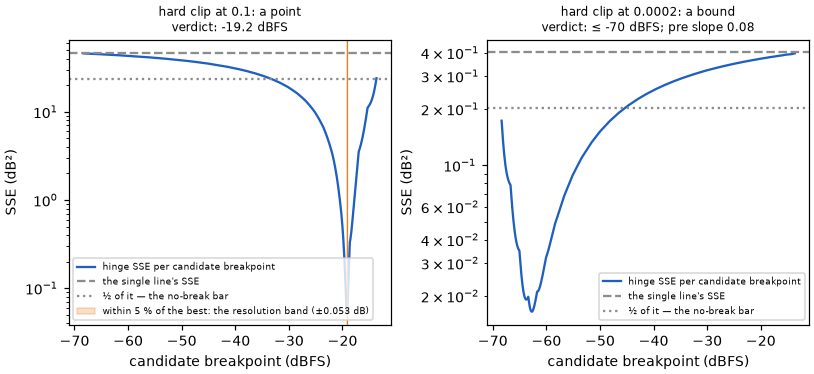
\includegraphics[width=0.95\linewidth]{compression-knee.png}
  \caption{How badly the two lines miss the rungs, for every candidate
  position of the corner. Left: a hard clipper whose threshold lies
  inside the ladder --- a sharp dip, a narrow band of positions that fit
  about as well, a number. Right: the same clipper with its threshold
  under the quietest rung --- the curve falls toward the bottom with no
  dip to trust, and the verdict is a bound at the quietest rung.}
  \label{fig:knee-plain}
\end{figure}

\paragraph{The hiss line.} A distortion reading is a ratio: the overtones
compared with the note. The hiss in the recording is a fixed amount,
while the note shrinks as the ladder goes down, so at the quiet end the
hiss is a larger and larger share of the note --- and some of it lands
where the overtones are read. The \term{noise-bound} is how much
distortion the hiss alone could fake at each rung, worked out as a
deliberately generous worst case: as if every bit of the hiss had landed
on the overtones. Anything under that line cannot be told from the rig,
and the line rises toward the quiet end. The stamp it is built from is
this capture's own, pedal included --- a calibration made with nothing in
the loop cannot carry the pedal's hiss, so no calibration figure enters
here, unlike the sweep measurements of the earlier chapters.

The hiss line has two possible companions. If the library holds a
\term{null-run-reference} --- the loop measured with nothing in it, by
this same measurement, under exactly this record's calibration --- the app
reads from it how much distortion the rig itself \emph{adds} at each
loudness. That contribution is an absolute amount, so it is scaled to how
loud this pedal's note actually came out: a pedal with gain stands
further above the same rig floor, and one that pads the signal stands
closer to it. It is read only between the null run's own quietest and
loudest rungs, never guessed beyond them. And a plugin has no rig hiss
at all --- its calibration is numerically silent --- so instead the app
measured the plugin's own noise before the run, and that
\term{operative-floor} stands in for the hiss. The line drawn on the
chart is the \emph{largest} of the bounds that apply, since each one
bounds something that is not this pedal's distortion and taking the
largest can only be more careful; the \term{floor-source} label names a
companion only where it actually sets the line somewhere, so that a null
run sitting under this capture's own hiss everywhere is not what the
reader is told they are looking at.

With the line drawn, every rung gets a \term{floor-class}. At or under
the line (within \cmpAtFloorEpsilonDB{}~dB), the reading \emph{is} the rig.
Above it but within \cmpClearMarginDB{}~dB, the reading is a mix of the
pedal and the hiss. Beyond that it is clear: the pedal. The trace is then
drawn in \term{floor-runs}: solid where it is clear, dotted where it is a
mix, faint where it is the hiss, each stretch between two rungs taking
the more cautious of its two ends' classes; and where the trace would fall
under the chart's own bottom edge it is left as a gap, never drawn as a
line along the edge that would look like a reading.
Figure~\ref{fig:floor-plain-cmp} shows all of it on a plain wire through a
little noise and a loop with a little distortion of its own.

\begin{figure}[htbp]
  \centering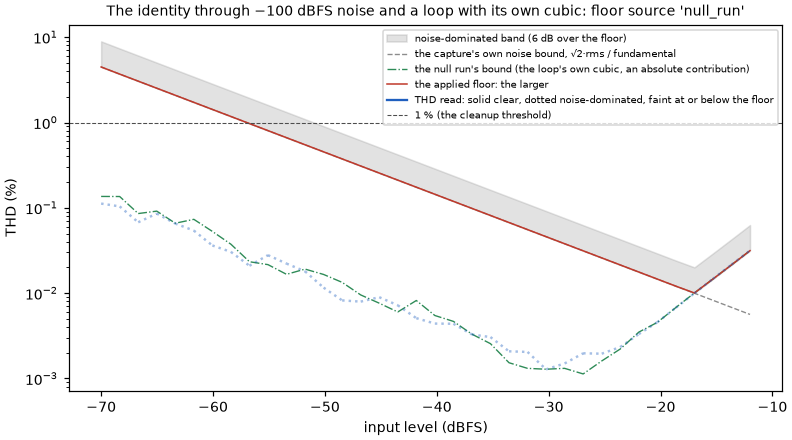
\includegraphics[width=0.95\linewidth]{compression-floor.png}
  \caption{The hiss line on a plain wire through a little noise and a
  loop that adds a little distortion of its own: the capture's own noise
  bound rising toward the quiet end, the null run's bound (the loop's own
  distortion, an absolute amount, defined only inside the rungs it
  measured), the line drawn as the larger, the band above it where a
  reading is a mix, and the trace in the chart's three styles --- here at
  or under the line everywhere, since a wire adds nothing of its own.}
  \label{fig:floor-plain-cmp}
\end{figure}

\paragraph{Does it clean up?} Read the distortion from the quietest rung
to the loudest. The cleanup reading says where, going up, it first crosses
the line of \cmpCleanupThresholdPercent{}\,\% --- a convention for reading
the curve, drawn where the app's own code draws it; the value is read out
of the app by probing the shipped rule rather than typed. The reading has
three states, and the ends of the ladder are never dressed up as a
crossing. If the quietest rung is already over the line, the pedal is
\emph{never clean} --- within this ladder's range, the only range it can
speak for. If some rung is the first over the line, the pedal
\emph{cleans up}, and the level is placed between that rung and the one
below in proportion to how far each sits from the line. If no rung
reaches the line, the pedal is \emph{always clean}, as far as this ladder
goes. Only a genuine crossing quotes a level or draws a marker.
Figure~\ref{fig:cleanup-plain-cmp} shows the three. The Gain Map chapter
that follows reads the same three states off each column of its map, by
the same rule.

\begin{figure}[htbp]
  \centering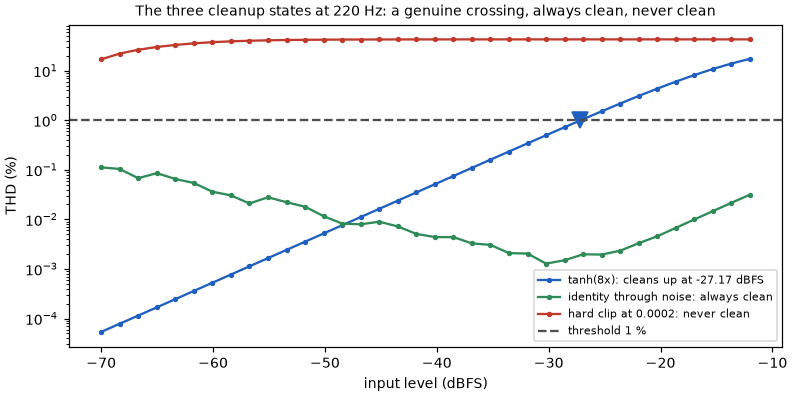
\includegraphics[width=0.85\linewidth]{compression-cleanup.png}
  \caption{The three cleanup states: the steep soft clipper crossing the
  line between two rungs (the triangle marks the crossing); a plain wire
  through noise that never reaches it; and a hard clipper whose threshold
  lies under the quietest rung, over the line at every rung.}
  \label{fig:cleanup-plain-cmp}
\end{figure}

\paragraph{Did the note come through?} Every distortion reading is a
ratio to the note, and a ratio to a note that is not there means
nothing. A few devices --- an octave-up effect at full tilt, a rectifier
--- remove so much of the note that what the estimator reads at the
note's own pitch is leakage from the louder overtones. Chapter one
measured how far below the loudest thing in a reading the note can sit
before that happens (\hdSeparationDB{}~dB), and each rung is judged by
that rule from the one distortion figure it stores: the
\term{summed-presence}, which compares the note with all its
overtones together rather than with the loudest one, and so is at most
\cmpSummedEagernessDB{}~dB quicker to call the note absent --- careful in
the direction of quoting less. If most rungs fail, no knee, no cleanup
level and no percentage is quoted for the record; the curve's shape is
still shown. The check at the end of the chapter runs a made-up device
with no note through it.

\paragraph{The summaries.} The generated summaries take four things from
the curve --- the knee's level, with a confidence that stays low for a
bound; how sharp the bend is, from how many dB of input the slope takes
to fall between two levels; the average slope over the top of the
ladder; and the cleanup reading, in the same three states --- and they are
a later chapter's subject. One more app-level fact belongs here: a
hardware record whose calibration carries the measured volts factor draws
its input axis and quotes its knee and its cleanup level in volts at the
pedal's input, and a plugin record's axis is digital full scale --- a
different physical quantity --- so no gap between the two is ever a
single number.

\subsection{The settings}

Every setting is in the technical reference's Compression chapter, in one
table read from the manifest. This chapter repeats the handful a reader
acts on. The hardware ladder runs from \cmpHardwareFloorDBFS{} to
\cmpHardwareCeilingDBFS{}~dBFS in \cmpHardwareSteps{} rungs
(\cmpHardwareStepDB{}~dB apart) and the plugin ladder from
\cmpPluginFloorDBFS{} to \cmpPluginCeilingDBFS{}~dBFS in
\cmpPluginSteps{} (\cmpPluginStepDB{}~dB apart); a fine window adds rungs
\cmpFineStepDB{}~dB apart, at most \cmpFineCap{} of them; the note is
\cmpNoteHz{}~Hz; each rung settles for \cmpSettleS{}~s (the first
\cmpRampS{}~s of it the ramp) and is measured for \cmpMeasureS{}~s,
trimmed to \cmpMeasureCycles{} cycles; the silence before the tone is
\cmpPrerollS{}~s; a rung within \cmpGateDB{}~dB of the hiss is dropped;
the corner's upper line must fall under \cmpSlopeThreshold{} of
one-for-one to count as a knee and its lower line must reach
\cmpUnityGuardSlope{} for the corner to be a number; the cleanup line is
\cmpCleanupThresholdPercent{}\,\%; and a reading is clear of the hiss
line at \cmpClearMarginDB{}~dB above it.

\subsection{What the result looks like}

The app's own chart, rendered from its chart code on its simulated pedal
(never a screenshot), is Figure~\ref{fig:app-compression}. Across the top
run three tiles: the probe note, with its frequency; the knee, as a level
in dBFS with the app's short gloss under it; and the cleanup level, with
its own gloss. Under them the Touch Response chart puts the input level
along the bottom --- labelled as how hard you hit the strings --- and the
output level up the side. The measured curve follows the dashed
one-for-one reference at the quiet end and then flattens; a dashed
vertical line marks where the pedal cleans up and another where the knee
sits, each labelled; and a shaded band across the right of the plot is
left unlabelled by the chart itself --- the user guide's Compression page
says what it marks. Below is the companion chart, Distortion vs.\ Level:
the distortion in percent against the same input axis, with the
\cmpCleanupThresholdPercent{}\,\% line dashed across it and labelled. On this record the trace
begins part-way across and the line under the chart says why: where the
measured distortion falls under the chart's own lowest mark it is left as
a gap, because the true values there are lower than anything the axis can
draw. This particular pedal is a simulated one, so it carries no noise
stamp and the chart draws no hiss line; on a hardware record the line,
the band above it and the three trace styles of the previous section
appear on this lower chart, and a legend names the floor's source.

\begin{figure}[htbp]
  \centering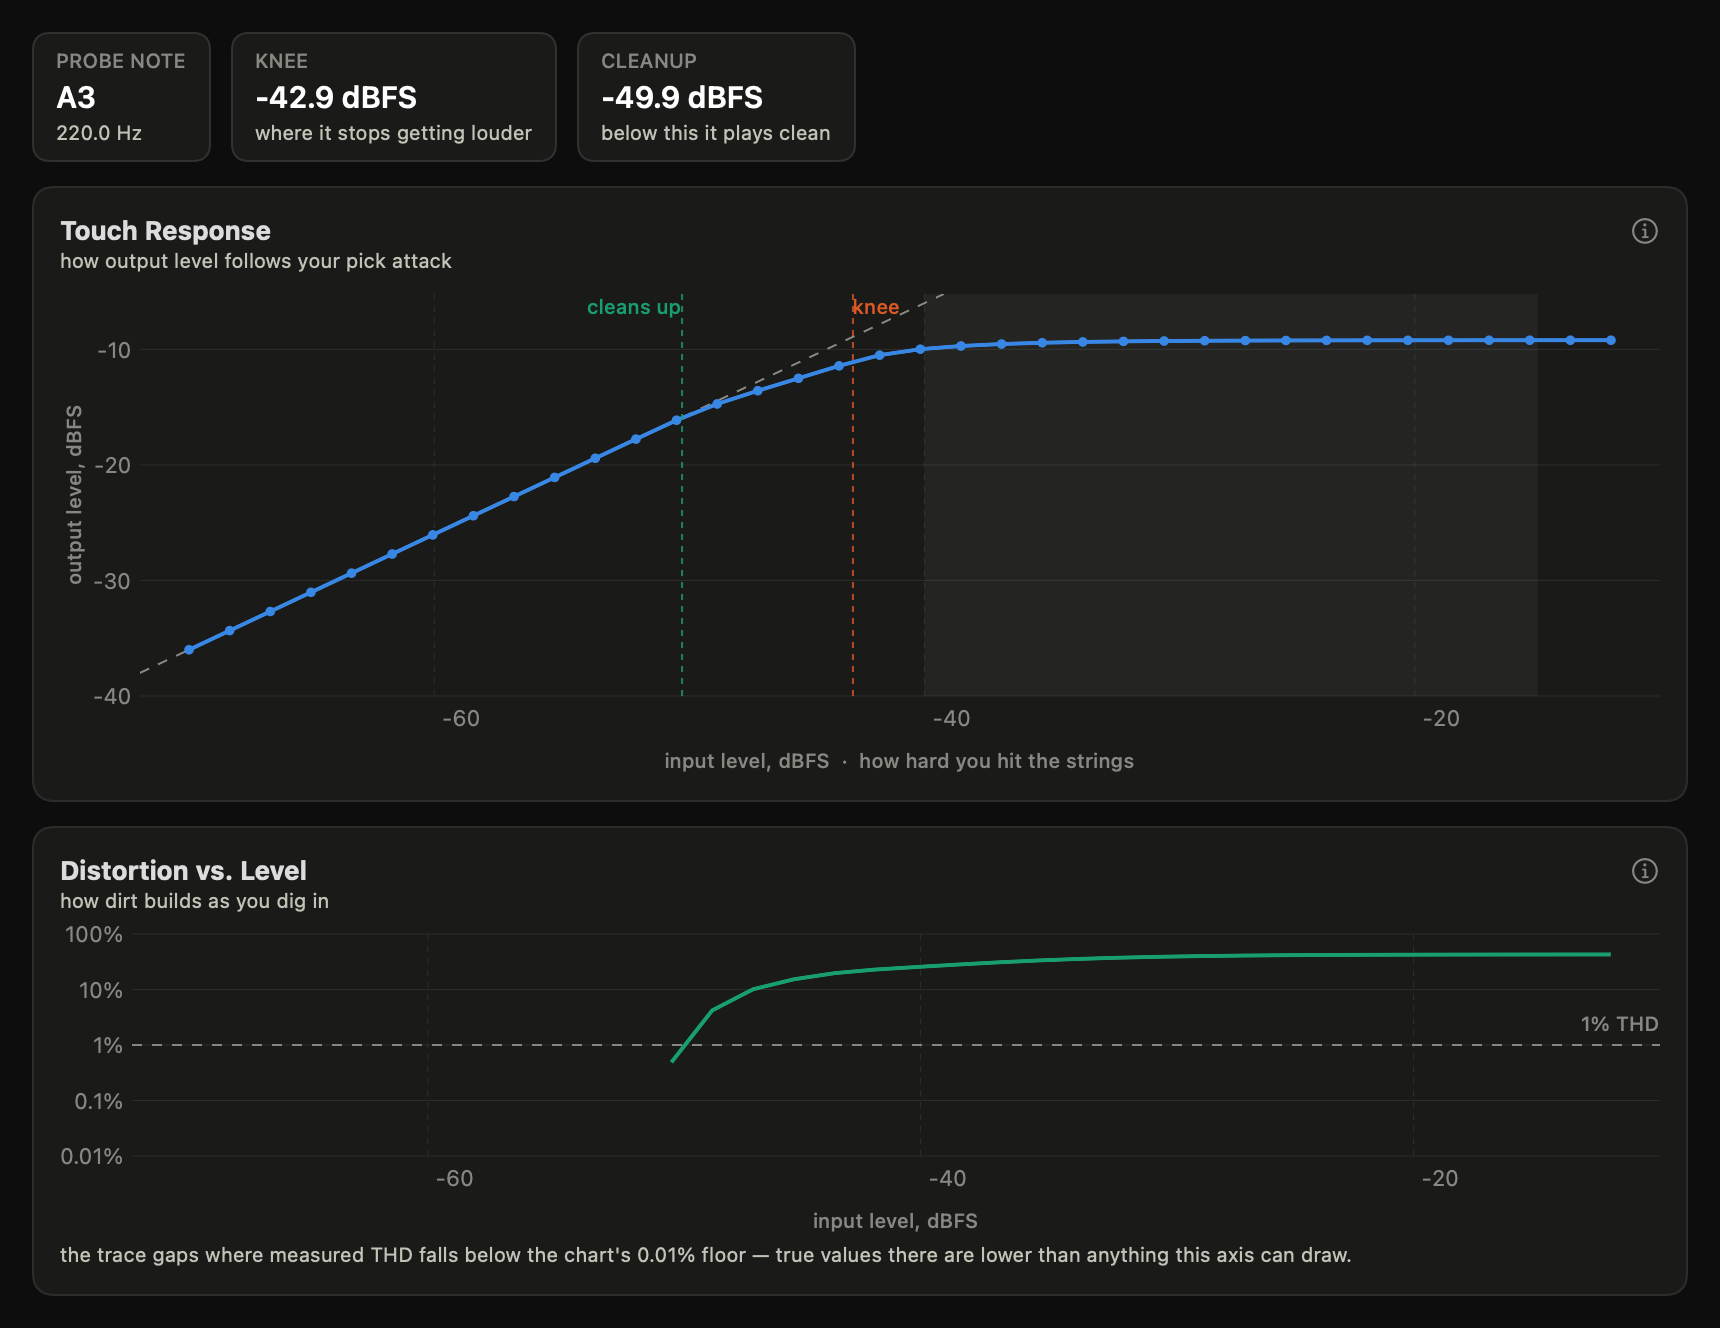
\includegraphics[width=0.85\linewidth]{compression--sim-knee.png}
  \caption{The Compression view as the app draws it, for its simulated
  pedal: the three tiles, the Touch Response chart with its one-for-one
  reference and its two markers, and the Distortion vs.\ Level chart with
  its gap under the axis floor.}
  \label{fig:app-compression}
\end{figure}

\subsection{How you can check that the app does what this says}

As in the earlier chapters, a second program was written from the
description --- in Python, independently, not by translating the app's
code --- and the \term{parity} runs both on the same made-up devices and
demands the same answer. It runs \cparityCaseCount{} cases, and two of
the device cases a second time as their \term{phantom} twins
(\cparityTwinCount{} twins). Every case is a known device through a known
loop: a delay, a stream of noise added at the interface's input, a gain
applied after them as an input knob would apply it, and, in some cases,
a little distortion of the loop's own, the way a converter adds some.
The Python borrows chapter one's devices and noise and the Transfer Curve
chapter's tone filters, and owns everything else: this instrument has no
sweep in it.

The known answer is chapter one's again. For a device with no memory, the
exact size of the note and of every overtone at any loudness can be
computed from the device's formula, so beside every rung the second
program prints the exact ladder of sizes at that rung's drive and the
exact distortion it implies; and for the read-time half it applies the
app's own rules --- the hinge fit, the cleanup reading, the hiss line ---
to those exact rungs, so the knee, the cleanup and every label have exact
answers too. A knee has no truth beyond that: it is a summary of a curve,
not a property of the device, and the check asks whether the app's
summary of the measured curve matches its summary of the exact one.

One idea is new here and worth a paragraph: the \emph{leakage
allowance}. The estimator's reading of one overtone picks up a trace of
its neighbours --- a little of the note, a little of the overtone next
door --- even on a stretch cut exactly, because the taper at the
stretch's ends is not perfect. How much depends only on how far apart
the two pitches are: \cparityLeakageOne{}~dB below the leaking pitch at
one overtone's distance, \cparityLeakageTwo{} at two, \cparityLeakageEight{}
at eight, the same at every loudness. That table is measured first, on a
made-up recording containing the note and nothing else, and it is
allowed for before any real case is judged: an overtone whose true size
sits close to what its neighbours leak into it can read a little off for
the estimator's own reasons, that much is subtracted from the
disagreement, and what remains is held to the bar. Under the final fade
the leakage rises to \cparityFadeLeakageOne{}~dB, which is why the last
rung is left out of every comparison and stated as a limit instead.

The demands, in numbers the pipeline writes into this document. The two
programs must agree at every rung and every overtone to within
\cparitySwiftToleranceWords{} of a decibel (\cparitySwiftTolerance{}~dB)
with no filter in the loop --- on the run that built this document the
worst disagreement was \cparityWorstSwiftWords{} of a decibel
(\cparityWorstSwift{}) --- and to within
\cparitySwiftFilteredToleranceWords{} (\cparitySwiftFilteredTolerance{})
through a filter (measured \cparityWorstSwiftFilteredWords{},
\cparityWorstSwiftFiltered{}); every yes-or-no reading --- each rung's
gate verdict, every floor class, every run, the knee's kind and level and
label, the cleanup state, the floor's label with and without a null run,
the presence verdict --- must be identical. On every noiseless case, at
every rung but the last, the app's reading of the note must sit within
\cparityHOneWords{} of a decibel (\cparityHOne{}) of the exact size
(measured \cparityWorstHOneWords{}, \cparityWorstHOne{}); the overtones,
once the leakage is allowed for, within \cparityTruthSmoothWords{}
(\cparityTruthSmooth{}) for the smooth devices (measured
\cparityWorstResidueSmoothWords{}, \cparityWorstResidueSmooth{}) and for
the hard clipper (\cparityWorstResidueKinkedWords{},
\cparityWorstResidueKinked{} --- at the probe note and rate no folded
overtone of a computed device lands on a pitch that is read, so the
clipper with a kink reads like a smooth one here), and within
\cparityTruthFilteredWords{} (\cparityTruthFiltered{}) through a filter
(\cparityWorstResidueFilteredWords{}, \cparityWorstResidueFiltered{}); and
the distortion figure, summed over exactly the overtones the app sums,
within \cparityTHDWords{} (\cparityTHD{}; measured
\cparityWorstTHDResidueWords{}, \cparityWorstTHDResidue{}). The knee must
land within \cparityKneeWords{} of a decibel (\cparityKnee{}) of the exact
curve's knee (measured \cparityWorstKneeWords{}, \cparityWorstKnee{} ---
every knee that is a number lands on the same candidate position on both
sides, and the two that differ do so by one candidate step), and the
cleanup crossing within \cparityCleanupWords{} (\cparityCleanup{};
measured \cparityWorstCleanupWords{}, \cparityWorstCleanup{}). The noise
stamp must read the injected noise within \cparityStampWords{} of a
decibel (\cparityStamp{}; measured \cparityStampErrorWords{},
\cparityStampError{}, the estimate's own scatter over a short silence).

Four checks are about the rig rather than the device. The same device and
the same noise through a loop turned up by a stated amount must move
every output level by exactly that amount --- the departure measured
\cparityGainShiftWords{} of a decibel (\cparityGainShift{}) --- and move
the knee's input level by \cparityGainKneeMoveWords{}
(\cparityGainKneeMove{}; the bar is \cparityGainWords{}, \cparityGain{}),
with every floor class unchanged: turning the interface up does not move
the knee, which is the point of reading the knee on the input axis. A
recording \cparityLatencyFound{} samples late, with the app told the
silence plus that delay, must read every rung as the undelayed recording
did, to \cparityLatencyMoveWords{} of a decibel (\cparityLatencyMove{};
bar \cparityLatencyWords{}). A stretch cut \cparityMiscutSamples{} sample
late must move the note's reading by no more than
\cparityMiscutWords{} of a decibel (\cparityMiscut{}; measured
\cparityMiscutMoveWords{}, \cparityMiscutMove{}) --- the taper makes a
one-sample miss invisible, which is what it is there for. And a phantom
with no note at all --- its note \cparityAbsentDepth{}~dB under its own
second overtone --- must read absent on most of its rungs (measured
\cparityAbsentFraction{} of them) and get no knee, no cleanup level and
no floor label; the same made-up recording measures how well the
estimator separates a note from its overtones on a cut stretch,
\cparitySeparation{}~dB against the \cparitySeparationBar{}~dB chapter
one's bound allows, which is why that borrowed bound is safe here by a
wide margin. \cparityPartBStatus

Two results are worth stating in words. The worked example, the steep
soft clipper with no noise on the hardware ladder: its knee is a number
at \cparityWorkedKnee{}~dBFS, resolution $\pm$\cparityWorkedKneeResolution{}~dB,
displayed as ``\cparityWorkedKneeLabel'', with a lower line of slope
\cparityWorkedPreSlope{} and an upper line of \cparityWorkedPostSlope{},
against the exact curve's \cparityWorkedTruthKnee{} (a difference of
\cparityWorkedKneeErrorWords{} of a decibel, \cparityWorkedKneeError{});
its cleanup crossing is \cparityWorkedCleanup{}~dBFS against the exact
curve's \cparityWorkedTruthCleanup{} (a difference of
\cparityWorkedCleanupErrorWords{}, \cparityWorkedCleanupError{}). And the
hard clipper: its flat top begins at \cparityClipOnset{}~dBFS, and the
fitted corner sits at \cparityClipKnee{}~dBFS,
\cparityClipKneeAboveOnsetWords{} of a decibel above where the clipping
starts (\cparityClipKneeAboveOnset{}), with an upper slope of
\cparityClipPostSlope{}. That gap is a measured relation between a fit's
corner and a clipper's onset, not a claim about either: two straight
lines through a curve that turns a corner gradually will place their
join a little past the first departure from one-for-one. With a fine
window laid over that knee the ladder delivers \cparityFineDelivered{}
rungs, the knee reads \cparityFineKnee{}~dBFS and moves by
\cparityFineKneeMoveWords{} of a decibel (\cparityFineKneeMove{}), its
resolution unchanged, because on both ladders the band of corners that
fit about as well is narrower than one candidate step, and the candidate
spacing is then what the fit resolves.

Three cases are constructed to be exactly what the reading rules are
for. An exact line that compresses a little everywhere and then breaks
reads ``\cparityBreakKnee'' with fitted slopes \cparityBreakPreSlope{} and
\cparityBreakPostSlope{}: the unity guard, doing its job. Simulation
Mode's own assembly on the worked example --- fewer rungs, shorter
settles, no silence before the tone --- reads its knee at
\cparitySimulationKnee{}~dBFS, resolution
$\pm$\cparitySimulationKneeResolution{}, \cparitySimulationKneeGap{}~dB
from the hardware assembly's knee on the same device: what interactive
quality costs. And the exact line that compresses a little everywhere
and never breaks is the finding the limits section states.

The test runs automatically on every change to the app, and the tables
and figures in both documents are regenerated on every change and
compared with the committed copies; the scripts and the instructions for
running them are in the repository named on the first page.

\subsection{Where it stops being a measurement}

\begin{itemize}
  \item \textbf{The last rung is read under the test's own fade.} The
  note fades out over one ramp, and the last rung's measured stretch ends
  where the note ends, so it holds the fade: the last rung's note reads
  \cparityWorstFade{} to \cparityLeastFade{}~dB relative to its exact size
  on the check's devices --- a few thousandths low --- and the estimator's leakage there rises from
  \cparityLeakageOne{} to \cparityFadeLeakageOne{}~dB. That is a fact about
  the test signal, not about any pedal. Moving the fade past the stretch
  would change the signal every existing record was measured with, and is
  reported rather than made.
  \item \textbf{The no-bend test can be decided by that fade.} The first
  of the four decisions compares how badly two lines miss the rungs with
  how badly one line does, as a ratio, and the ratio has no scale of its
  own. On a curve that is one exact straight line, compressing a little
  everywhere, the only rung off the line is the last one under the fade;
  the two-line fit absorbs that one rung, the ratio reads ``a bend'', and
  the second decision then reads ``no knee'' --- where the same exact line
  with no fade reads ``at or below the quietest rung''. Measured on this
  build: the exact line reads ``\cparityLineMeasuredKnee'' on both programs
  while its exact curve reads ``\cparityLineTruthKnee'' with a slope of
  \cparityLineTruthPreSlope{}. A measured pedal rarely draws an exact
  line, and any real curvature outweighs one bent rung, so the case is
  stated as one the fit decides on structure the test cannot see, and
  left as a finding.
  \item \textbf{A rung skipped because its stretch ran past the recording
  is silent.} It leaves no point and no count, unlike a rung the gate
  dropped; a short recording simply yields a shorter curve.
  \item \textbf{Simulation Mode builds its test differently.} No silence
  before the note, so no noise stamp and no hiss line; fewer rungs and
  shorter settles at its quick quality (\cmpSimInteractiveSteps{} rungs,
  \cmpSimInteractiveSettleS{}~s to settle and \cmpSimInteractiveMeasureS{}~s
  measured, at \cmpSimInteractiveRateKHz{}~kHz, against the hardware
  assembly's \cmpHardwareSteps{}, \cmpSettleS{}~s and \cmpMeasureS{}~s, at
  \cmpSampleRateKHz{}~kHz in the check); its full quality uses the hardware assembly's
  rungs and settles. On the worked example the quick quality's knee sits
  \cparitySimulationKneeGap{}~dB from the hardware assembly's, so a
  simulated record and a measured one agree on the shape of a curve and
  not on the last decibel of its knee, and a comparison between the two is
  read that way.
  \item \textbf{A soft onset is not disclosed.} The unity guard tells a
  clean anchor from a missing one; it does not tell a wide, gradual bend
  from a sharp corner. A pedal whose bottom decade is clean and whose bend
  then spreads over many dB gets a knee that is a number and is honest as
  far as the fit goes; how wide the bend is would be a new reading, not a
  tighter one.
  \item \textbf{The quiet end is the rig's.} Under the hiss line a
  reading is the rig, and the rungs say so one by one; a rise in
  distortion toward the quiet end is the hiss's growing share of a
  shrinking note, not the pedal, unless it stands clear of the band.
  \item \textbf{The loudness axis is the signal, never a knob.} How loud
  the note goes in is how hard the circuit is driven; the pedal's knobs
  stay where you set them, and a knob is measured one curve per position.
  \item \textbf{One note.} The curve is one pitch; a pedal with a tone
  network ahead of its clipper compresses differently at another, and the
  Gain Map (Section~\ref{sec:journey-plain}) is the cross-check across
  notes.
  \item \textbf{The simulated pedal folds its own overtones.} A device
  computed sample by sample makes overtones above half the sample rate
  that fold back into the band. At the probe note and rate none of them
  lands on a pitch that is read, and the check's phantom twins are the
  fold-free control; at another note or rate the highest overtones of a
  computed device with a kink in it would not be the exact answer there.
\end{itemize}

\clearpage
\section{Gain Map}
\label{sec:journey-plain}

\subsection{What this measurement tells you, and what it cannot}

The Harmonic Distortion measurement of Section~\ref{sec:hd-plain} asks
one question at one loudness: play a note into the pedal at a stated
level, and list the harmonics that come out. But a distortion pedal is
not one thing at all loudnesses. Play it softly and it may pass the note
almost untouched; dig in and it clips; somewhere between the two it
changes. A \term{gain-map} asks chapter one's question again at each rung
of a ladder of loudnesses --- one sweep per rung, each analysed on its own
--- and draws the answers as a map: how hard the pedal is driven up one
side, which note you play along the other, and one square per loudness
and note holding the distortion the pedal made there.

\paragraph{Loudness as an axis.} The new axis needs a sentence of its
own, because it is easy to mistake for a knob. The \term{drive-level} of a
row is how hard the app drives the pedal --- the level of the test signal
going into it, as your pick and your guitar's volume knob would drive it.
The pedal's own knobs are never touched while a map is measured; they
stay wherever you set them, and that setting is recorded with the
measurement. So the vertical axis is not the drive knob. It is the thing
the drive knob is turned to suit: the signal arriving at the circuit. To
map what a knob does, you measure one map per knob position. The rungs of
the ladder are the \term{level-lattice}, and the quietest and loudest
rungs are its \term{drive-window}.

Figure~\ref{fig:column-plain} is the whole idea in one picture, computed
from the worked example of the earlier chapters --- the soft clipper of
the \term{tanh} curve --- through the pipeline described later. On the
left is one \term{map-cell}: one note, one loudness, and the ladder of
harmonics the analysis reads there, exactly chapter one's picture at one
point of the range. In the middle is the same note at every rung of the
ladder, the ladder of harmonics growing rung by rung as the pedal is
driven harder. On the right is the whole map, with that column and that
cell outlined. A cell is one measurement; a column is the rungs of one
note stacked; a map is the columns side by side. Everything the rest of
this chapter says is about how those cells are filled in and which of
them may be believed.

\begin{figure}[htbp]
  \centering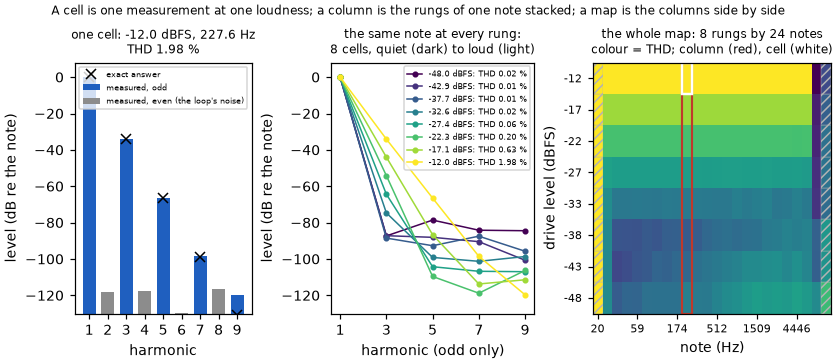
\includegraphics[width=0.98\linewidth]{explained-column.png}
  \caption{A map is a stack of single-loudness measurements. Left: one
  cell of the worked example --- the soft clipper at the loudest rung of
  the hardware ladder, at the note the cleanup tile reads --- as the
  measured level of each harmonic relative to the note (blue for the odd
  harmonics, grey for the even ones, which this clipper does not make and
  which read the loop's own noise), with the exact answer marked by a
  cross; the ninth harmonic's exact answer lies under the loop's noise,
  just below the pane. Middle: the same note at all \gmLevels{} rungs,
  quiet to loud, each rung's THD in the legend. Right: the whole map, THD as
  colour, the fade columns hatched, the column outlined in red and the
  cell in white.}
  \label{fig:column-plain}
\end{figure}

When a map is opened, the app states three things beside it, each worked
out afresh from the stored squares: the \term{peak-tile}, the most
distortion the pedal clearly made anywhere on the map, or a bound when
nothing clearly stands out; the \term{cleanup-reading}, where, going up
the ladder at one note, the pedal starts to distort; and the
\term{fundamental-presence} verdict, whether the note itself survived
well enough for any ratio to it to mean anything. Each has its own
section below.

\paragraph{What it cannot tell you.} Stated once.
\begin{enumerate}
  \item \textbf{Nothing about the pedal's own volume or gain.} Every
  square is a ratio: the harmonics compared with the note itself, in that
  square. A pedal that is loud and clean and one that is quiet and clean
  draw the same square. And the vertical axis is the signal driving the
  circuit, never a knob on it.
  \item \textbf{Nothing between two rungs.} Each rung is its own capture,
  seconds apart from the next. A pedal whose behaviour drifts or sags
  between them --- a dying battery, a warming transistor --- shows the
  drift as a wobble from row to row, which the map draws and does not
  name.
  \item \textbf{Whether a square near the floor is the pedal or the rig.}
  Below the margin described later, a square is quoted as a bound ---
  ``no more than this'' --- never as a figure.
  \item \textbf{Nothing in the two fade columns.} The first and last notes
  of the map sit inside the sweep's fade-in and fade-out, and what they
  show is the test signal, not the pedal.
  \item \textbf{Nothing a short column lost.} Near the top of the map some
  of a note's harmonics lie too high to be counted honestly, and that
  column's distortion figure is known to be short.
  \item \textbf{Nothing about listening.} The map says how much distortion
  there is at each loudness and note. It says nothing about what the distortion sounds like.
\end{enumerate}

\subsection{The test signal, and the ladder of loudnesses}

The ladder first. On a hardware rig the map is measured at
\gmLevels{} rungs, from \gmHardwareFloorDBFS{} to
\gmHardwareCeilingDBFS{}~\term{dbfs}, a span of \gmHardwareTravelDB{}~dB
climbed in equal steps of \journeyHardwareStep{}~dB. Equal steps in
decibels are equal \emph{ratios}, not equal amounts: each rung is the same
proportion louder than the one below. The top rung is held back from full
scale on purpose. An interface's input has to be set so that the pedal's
output never clips the converter at the loudest drive; with the input
staged that way, the top rung is the loudest drive that cannot clip it,
and the ladder reaches down a fixed span below. A plugin has no
converter to protect --- it is arithmetic on numbers --- so its ladder
runs to the very top, from \gmPluginFloorDBFS{} to
\gmPluginCeilingDBFS{}~dBFS in steps of \journeyPluginStep{}~dB, its
quietest rung lower still, down where high-gain plugin amplifiers were
measured to start bending.

At each rung the test signal is the same gliding tone as chapter one's
--- the \term{sweep}, from \gmStartHz{} to \gmEndHz{}~Hz, with the same
fades --- at that rung's loudness. There is one difference that matters
later: by default each rung's sweep lasts \gmSweepDefaultS{} seconds,
\gmSweepShareOfFingerprint{} the \hdRequestedDurationS{}~seconds of
chapter one's, because \gmLevels{} sweeps take \gmLevels{} times as long; the measure
sheet offers \gmSweepChoicesS{} seconds, and the length chosen is not
written into the record. Each sweep is played after \gmPrerollS{}~s of
silence and followed by \gmTailS{}~s more, and the analysis that reads it
is also \gmTransformShareOfFingerprint{} as fine as chapter one's. A
shorter sweep is a coarser instrument: the analysis's own small residue
--- the distortion it reports with nothing in the loop --- is larger for
it, and a later section says by how much.

The notes the map is drawn at are chosen once, as a grid: \gmGridCount{}
of them, spaced by equal musical intervals --- \gmColumnSemitones{}
semitones, \gmColumnOctaves{} of an octave --- from the lowest note the
sweep plays to the highest. That is the \term{export-grid}. Its first and
last columns sit exactly at the sweep's two ends, inside the fades, which
is why those two columns are masked, as the next section explains.

The rungs are played and recorded one after another, and each recording
is analysed entirely on its own, as if it were the only sweep. Nothing about one rung leaks into another. Figure~\ref{fig:map-plain}
is what the measurement produces: the worked example's map, computed by
the pipeline through a loop with a little noise in it, coloured by
distortion and marked with the tiles the later sections explain.

\begin{figure}[htbp]
  \centering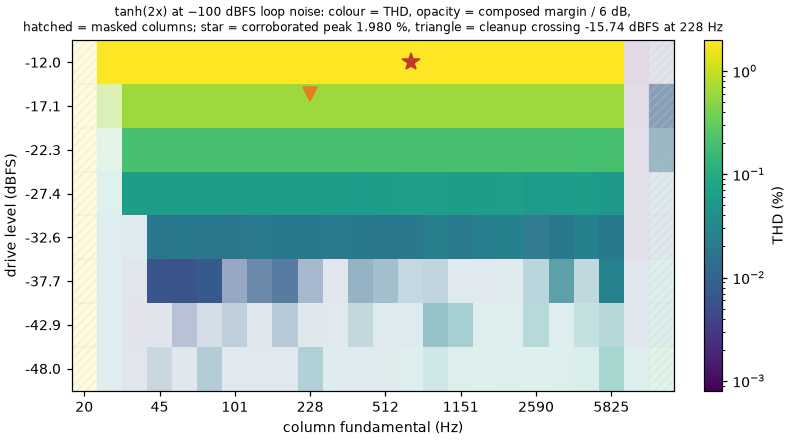
\includegraphics[width=0.95\linewidth]{journey-map.png}
  \caption{The worked example's map: the soft clipper on the hardware
  ladder through a loop with a little noise. Colour is THD; a square is
  drawn fainter the less clearly it stands above the floor described in
  the next section; the two fade columns are hatched; the star is the
  peak the tile quotes and the triangle is where the cleanup reading
  places the crossing at the tile's note.}
  \label{fig:map-plain}
\end{figure}

\subsection{How the map is built}

Five steps, each in words; the technical reference gives the exact rule
for each.

\paragraph{Cutting each recording to size.} Every signal through a rig
comes back a little late --- the round trip through the converters and
cables. The calibration measured that delay, and each rung's recording
is cut at the moment the sweep is known to have arrived: the silence
before it dropped, the sweep and the silence after it kept, and never a
sample past the recording's end. A plugin measures its own delay on every
render and hands back a recording with none. The delay is never guessed.

\paragraph{Reading each rung as chapter one does.} Each cut recording
goes through exactly the analysis of Section~\ref{sec:hd-plain}: the
glide undone, each harmonic's blip cut out with its own window, and every
harmonic read against frequency. The app reads \gmHarmonicCount{}
harmonics at each rung, and the note's level along with them. Nothing is
corrected for the rig here: the loop's own gain and tone stay in every
reading, so a square's note level is the level the note actually reached
at the interface, with everything the loop added --- its
\term{delivered-fundamental}. That number is a level, not a reference,
and the floor's arithmetic in the next section leans on it.

\paragraph{Filling the squares.} For each rung and each note of the grid,
the app reads the \term{thd} over the audible band (\gmAudibleLowHz{} to
\gmAudibleHighHz{}~Hz), exactly as chapter one defines it, and the level
of each \term{harmonic-order} at that note. A harmonic that would lie
above half the sample rate, or a note at which the fundamental reads
nothing, leaves its square empty rather than wrong.

\paragraph{Masking what the test made.} Two columns are marked as the
test's own: the first and the last, which sit within a quarter tone
(\gmEdgeGuardCents{}~cents) of the sweep's two ends and were therefore
excited while the tone was still fading in or already fading out. A
plain wire shows the same readings there, so they describe the
measurement and not the pedal. They wear an \term{edge-mask}: drawn
faint, kept out of every headline number, and never allowed to set the
colour scale. A third kind of column is marked near the top of the map: a
\term{truncated-column}, where some harmonic that the audible band would
count lies past its \term{validity-bound}, so the column's distortion
figure is known to be short. It is flagged and kept out of the tiles,
never corrected.

\paragraph{What is stored, and what is not.} The record keeps the grid
of numbers --- every square's THD and harmonic levels --- the rungs, the
harmonics read, the sample rate and the band, and beside them one
\term{audition-model} per rung, a separate model of the pedal at that
loudness that only the listening panels use. Nothing described in the
next section is stored: every verdict below is worked out afresh each
time the record is opened, so a better rule corrects every map ever
made. A record from before the sample rate and the band were stored
derives no masks and no residue, and its squares summed every harmonic
below half the sample rate; the app treats it as the older reading it is.

\subsection{What the app decides when it reads a record back}

\paragraph{A floor, and a margin.} Everything the app says about a map
rests on one question, asked of every square: how far above the largest
thing that could fake it does this square's distortion stand? A square is
called a measurement only while it stands clear of \emph{every} fake at
once; below that it is a bound. The distance is the square's
\term{composed-margin}, and the things that could fake it are three.

The first is the loop's own noise. During calibration the app played its
sweep through the rig with a cable in place of the pedal and kept a note
of how much distortion and noise the bare loop showed at each pitch ---
the \term{floor-stamp}, stored inside every record made with that
calibration. It is a single reading at each pitch, and a single reading
can be unlucky, so the map reads it through a \term{median-read}: at each
pitch the stamp is replaced by the middle value of \gmStampMedianPoints{}
neighbouring points on its own grid, \gmStampMedianSide{} to either side,
\gmStampMedianOctavesWords{} of an octave (\journeyStampMedianOctaves{})
each way. That is wide enough that one unlucky trough cannot make the
loop look quieter than it is, and about as wide in all as one column of
the map, so a feature a column can resolve is not smoothed away. Then
comes an allowance, the \term{drive-term}, for the fact that the
calibration was checked at one loudness (\gmCalibrationLevelDBFS{}~dBFS)
and the map's squares are at many. Noise is a fixed amount, not a fixed
share: the same hiss is a bigger share of a quieter note. So a square
whose note arrived quieter than the calibration's did is given a floor
that much higher. A square whose note arrived louder gets no allowance in
the other direction --- the floor is never pushed lower than the
calibration measured, because the rig's own distortion grows with drive
and the calibration measured noise and distortion together at one level.
The comparison uses the delivered fundamental, the level the note
actually reached, and the calibration's own level plus the gain the loop
was measured to add; leave that gain out and every margin comes out
better than it is.

The second, on a plugin, is the plugin's own noise. A plugin's
calibration is a loop with nothing in it and no converters, numerically
silent, so it measures nothing the plugin does; instead the app measured
the plugin's own noise before the run, and that \term{operative-floor}
stands in for the loop noise a hardware rig would have.

The third is the one a noise floor cannot see: the \term{analyzer-residue},
the distortion the analysis itself reports with nothing at all in the
loop. Take the sweep, hand it straight back as its own recording, and
analyse it: a perfectly clean signal should read no distortion, and
almost everywhere it does. But at the first note after the masked
column, the sweep's fade-in ramp leaks into the window that reads the
second harmonic, and the analysis reports a little distortion that is
entirely its own. It is a fixed share of the note, not a fixed amount
--- it is the same at every rung --- which is exactly why a noise floor
cannot bound it. It shrinks as the sweep gets longer: at
\journeyResidueColumnOneHz{}~Hz it reads \journeyResidueColumnOneFive{}~dB
below the note on the default sweep, \journeyResidueColumnOneTwo{} on the
shortest and \journeyResidueColumnOneTen{} on the longest, and one column
higher it has already fallen to \journeyResidueColumnTwoFive{}, under any
real rig's noise. The app works the residue out afresh for each map's
own grid. Because the sweep's length is not written in the record, it
assumes the worst --- the shortest sweep the sheet offers, so the first
unmasked column is floored at \journeyResidueWorstColumnOne{}~dB on every
record --- a claim it can make about any record, at the price the last
section states. The left panel of Figure~\ref{fig:residue-plain} shows the
residue at every column for the three sweep lengths; the right panel is
the parity's own instrument, explained later.

\begin{figure}[htbp]
  \centering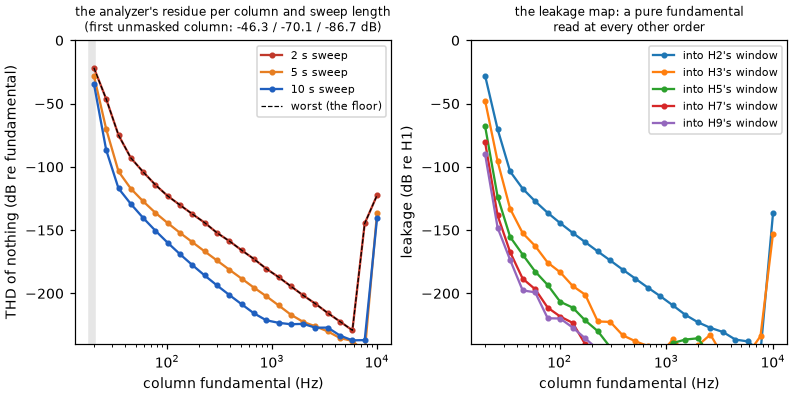
\includegraphics[width=0.95\linewidth]{journey-residue.png}
  \caption{Left: the analysis's own residue at every column of the map
  for the three sweep lengths --- the fade-in leak at the first unmasked
  column, largest on the shortest sweep --- and the worst case the record
  assumes (dashed). Right: the leakage map used by the check described
  later: a signal containing only its note, read at every other
  harmonic.}
  \label{fig:residue-plain}
\end{figure}

The composed margin is the square's distance above the \emph{largest} of
the three, because the largest fake is the one that binds. A square
clears when that distance is at least \gmMinimumMarginDB{}~dB.
Figure~\ref{fig:floor-plain} is the picture of it at one note of the
worked example. On the left, against loudness: the square's own THD
falling as the drive is turned down, the loop's floor read through the
median (with the single-reading version beside it), rising at the quiet
rungs by the drive term and flat above the calibration's level, the
analysis's residue far below at this note, and, on the right-hand scale,
the margin --- how far the square stands above whichever floor is higher
--- against the minimum. On the right, the same at the loudest rung
across every note.

\begin{figure}[htbp]
  \centering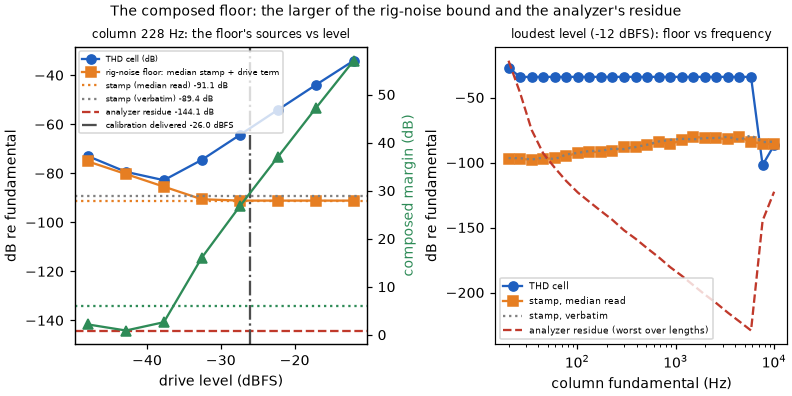
\includegraphics[width=0.95\linewidth]{journey-floor.png}
  \caption{The floor, composed from its sources, at one column of the
  worked example (left): the square's THD against loudness, the
  calibration's floor read verbatim and through the median, the drive
  term rising below the calibration's own level and flat above it, the
  analysis's residue, and the margin (green, right-hand scale) against
  its minimum. Right: the same at the loudest rung against note.}
  \label{fig:floor-plain}
\end{figure}

\paragraph{Is the note there?} Every square is a ratio to its own note,
and a ratio to a note that is not there means nothing. A few devices ---
an octave-up effect at full tilt, a rectifier --- remove so much of the
note that what the analysis reads at the note's own frequency is its own
leakage from the louder harmonics. Chapter one measured how far below
the loudest thing in a reading the note can sit before that happens
(\hdSeparationDB{}~dB), and each square is judged by that rule on its
own: present, absent, or undetermined when the note read nothing. The
map's verdict is then a majority over every square outside the two fade
columns, and it outranks the peak tile: when most squares have no note,
no percentage is quoted at all, only how deep the note sits. The verdict
is a majority for a reason the check at the end of this chapter shows.
On a device that has no note at all, a few squares still read
``present'' honestly --- at the quietest rungs the note's window holds
the loop's noise, and beside the low edge it holds the second harmonic's
own leakage --- and one square's truth must not overrule the map's.

\paragraph{The peak tile.} The headline number is the loudest square that
can be believed, and belief takes two steps. First, the fade columns and
the truncated columns are set aside, and so is every square whose note is
absent; among what remains, a square is \emph{clear} when its composed
margin reaches the minimum. Second --- and this is the step that keeps a
clean pedal from reading a number --- a clear square counts only when
the square one column beside it, the same rung one note away, is also
clear. That is a \term{corroborated-peak}. Real distortion spills onto
the neighbouring notes: a circuit that clips at one drive clips the note
next door too, and distortion changes slowly from one column to the
next. A noise reading happens to one square alone. The neighbour is asked
for along the note axis and never along the loudness axis, because
distortion can change a great deal from one rung to the next --- a
genuine onset at the loudest rung may have no clearing rung beneath it
--- while two noisy squares in adjacent rungs of one column are as likely
as any other pair.

The tile can therefore say one of three things. If any corroborated
square exists, the loudest of them is the peak: the most distortion the
pedal clearly made. If none does but some unmasked square has a figure,
the loudest of those is quoted as a bound, written with $\le$: the pedal
made no more than this, and the rig could not see under it. If the note
is absent over the map, no percentage at all. The bound is what a very
clean pedal earns, and it is not a small number: a plain wire through a
quiet loop reads a bound of \jparityIdentityBound{}\,\% on the default
sweep, because that is what the loop's noise adds up to at the loudest
of \gmCellCount{} squares, and nothing under it can be told
from the rig. Figure~\ref{fig:peak-plain} shows the rule deciding: on
the left, a plain wire through noise, where no square clears and the
tile is a bound; on the right, the soft clipper through the same loop,
where every clear square has a clear neighbour and the tile is a peak.
One case is left open on purpose: a map with no floor information at all
--- Simulation Mode, or a record made with no calibration --- has nothing
to judge its squares against, so every square counts as clear and
corroborated, and the tile states the loudest one as a peak. That is
reported rather than changed, and the last section returns to it.

\begin{figure}[htbp]
  \centering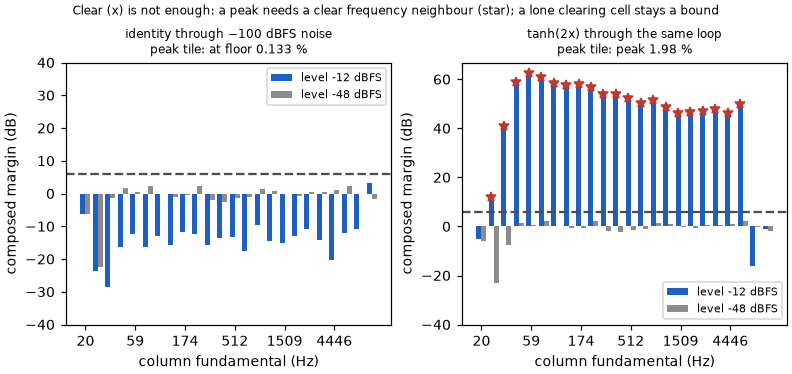
\includegraphics[width=0.95\linewidth]{journey-peak.png}
  \caption{The corroboration rule. Each panel shows the composed margin
  at every column for the loudest rung (blue) and the quietest (grey)
  against the minimum (dashed); a cross marks a square that clears on
  its own, a star one whose neighbouring note clears too. Left: a plain
  wire through a little noise --- nothing clears, and the tile is a
  bound. Right: the soft clipper through the same loop --- every clear
  square has a clear neighbour, and the tile is a peak.}
  \label{fig:peak-plain}
\end{figure}

\paragraph{Does it clean up?} Take one column of the map and read its
THD from the quietest rung to the loudest. The \term{cleanup-reading}
says where, going up, the pedal crosses the line of
\gmCleanupThresholdPercent{}\,\% distortion --- a convention for reading
the map, drawn where the app's own code draws it; the value is read out
of the app rather than typed, by probing the shipped rule until it
answers. The reading has three states, and the endpoints are never
dressed up as a crossing. If the quietest rung is already over the line,
the pedal is \emph{never clean} --- within this map's range, which is
the only range the map can speak for. If some rung is the first over the
line, the pedal \emph{cleans up}, and the level is placed between that
rung and the one below in proportion to how far each sits from the line.
If no rung reaches the line, the pedal is \emph{always clean} --- again,
as far as this map goes. The tile beside the map reads the column
nearest \gmCleanupTileHz{}~Hz (\gmCleanupTileNote), the note the
Compression measurement probes, so the two records' cleanup figures are
about one pitch; every other column carries the same three-state reading
too, and the chart's markers draw the genuine crossings. When the tile
says never clean, its subtitle says which range it means, and when the
pedal's own Compression record --- which probes further down --- finds a
genuine crossing below the map's floor, the subtitle points there
instead. Figure~\ref{fig:cleanup-plain} shows the three states at the
tile's note: the soft clipper crossing the line between two rungs, a
plain wire never reaching it, and a clipper whose threshold sits under
the ladder's quietest rung.

\begin{figure}[htbp]
  \centering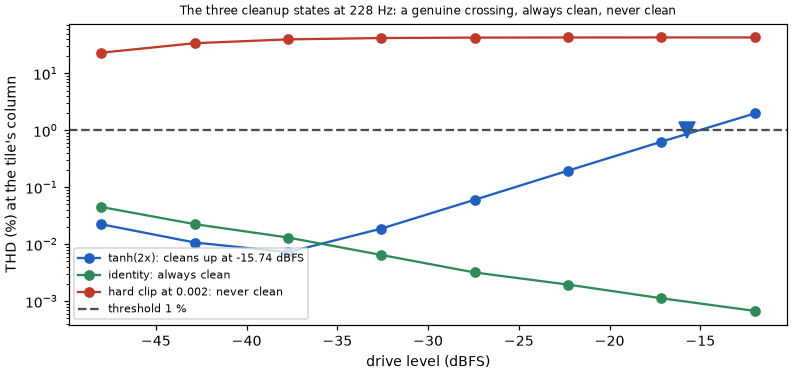
\includegraphics[width=0.85\linewidth]{journey-cleanup.png}
  \caption{THD against loudness at the tile's column for the three
  cleanup states: the soft clipper crosses the line between two rungs
  (the triangle marks the crossing); a plain wire stays under it
  throughout; a hard clipper is over it at every rung.}
  \label{fig:cleanup-plain}
\end{figure}

\subsection{The settings}

Every setting is in the technical reference's Gain Map chapter, in one
table read from the manifest. This chapter repeats the handful a reader
acts on. The hardware ladder runs from \gmHardwareFloorDBFS{} to
\gmHardwareCeilingDBFS{}~dBFS in \gmLevels{} rungs
(\journeyHardwareStep{}~dB apart) and the plugin ladder from
\gmPluginFloorDBFS{} to \gmPluginCeilingDBFS{}~dBFS
(\journeyPluginStep{}~dB apart); the sweep lasts \gmSweepDefaultS{}~s by
default, with \gmSweepChoicesS{}~s offered and the choice not stored; the
map has \gmGridCount{} note columns; the calibration's floor is read
through a median of \gmStampMedianPoints{} points; a square clears at a
margin of \gmMinimumMarginDB{}~dB; and the cleanup line is
\gmCleanupThresholdPercent{}\,\%, read at the column nearest
\gmCleanupTileHz{}~Hz.

\subsection{What the result looks like}

The app's own chart, rendered from its chart code on its simulated pedal
(never a screenshot), is Figure~\ref{fig:app-journey}. Across the top run
three tiles: the drive range, with the number of rungs measured; the
cleanup reading at \gmCleanupTileNote{}, with a line saying which range
the verdict covers; and the peak distortion, with a line saying it is the
loudest THD anywhere on the map. The chart itself puts the drive level up the
side, labelled so that up is digging in, and the note you play along the
bottom, named with its frequency; each square's colour is its THD, with
the scale under the chart running from the map's own faintest square to
its strongest, in percent, and the legend saying that a faded column is
a band edge --- the outermost columns are drawn faded. This particular
map is the app's simulated pedal at a setting that is over the cleanup
line at every rung, as its middle tile says. Figure~\ref{fig:map-plain}
above is the same kind of map as the pipeline
draws it, with the margins, the masks and the tiles' marks made visible.

\begin{figure}[htbp]
  \centering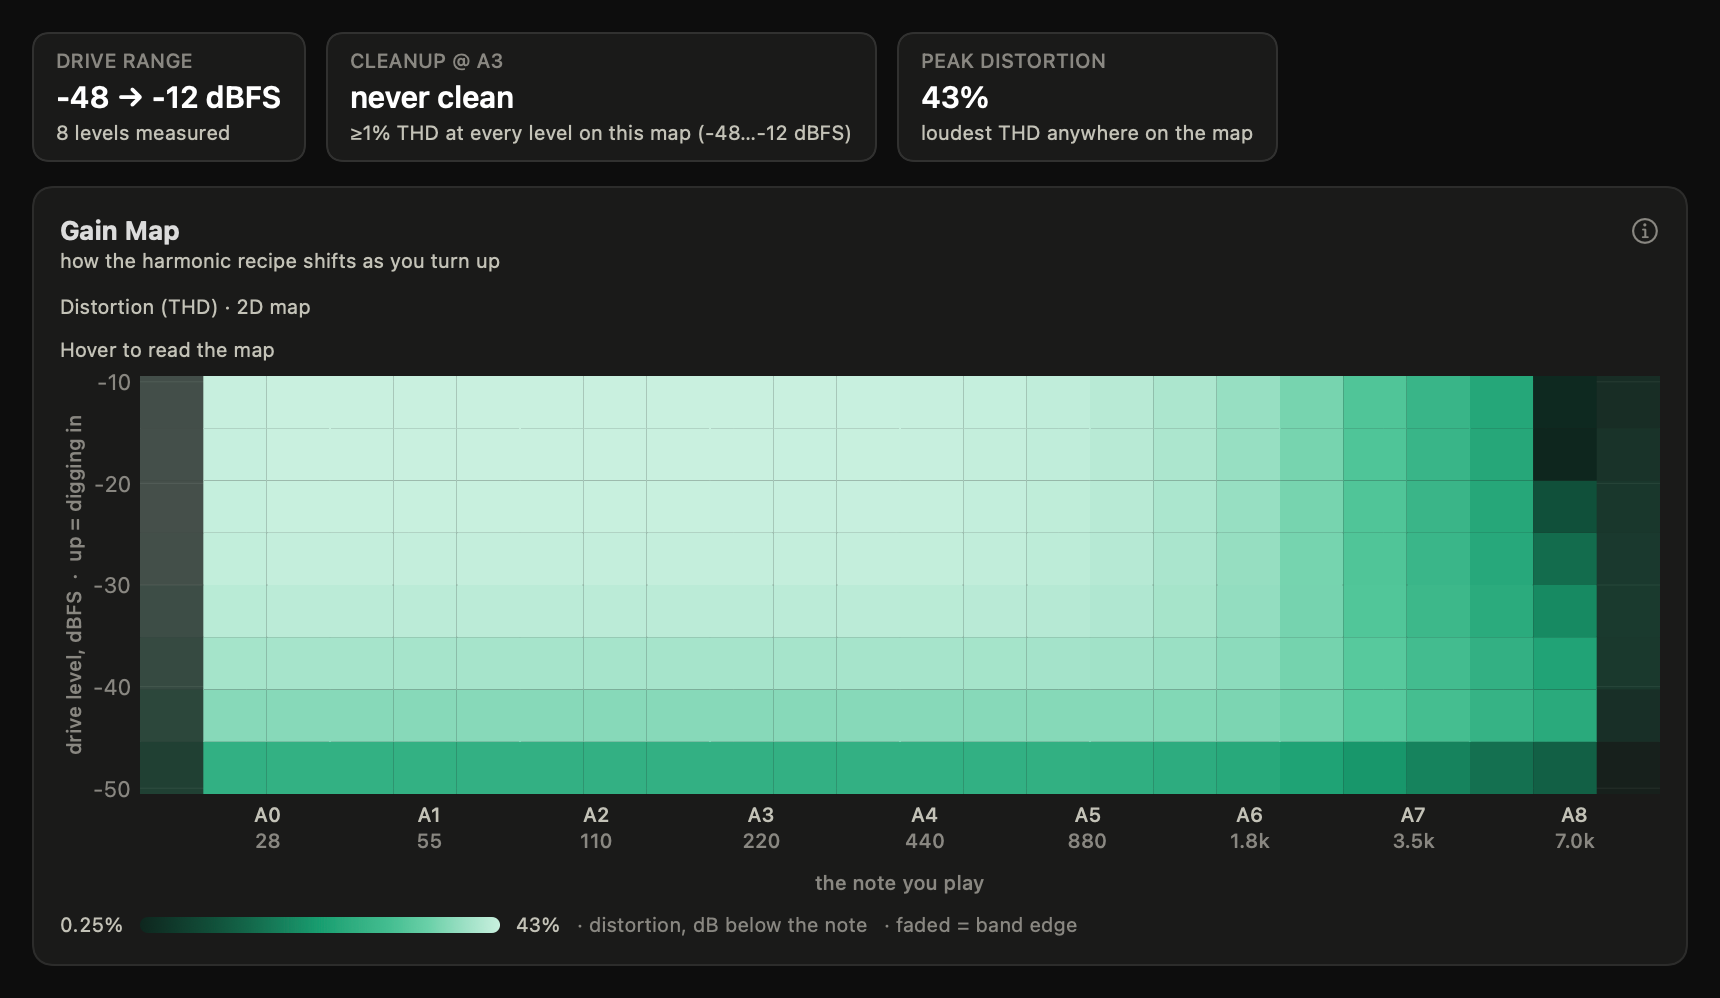
\includegraphics[width=0.85\linewidth]{gain-map--sim-thd-map.png}
  \caption{The Gain Map view as the app draws it, for its simulated
  pedal: the three tiles, the THD map over note and drive level, and the
  outermost columns drawn faded.}
  \label{fig:app-journey}
\end{figure}

\subsection{How you can check that the app does what this says}

As in the earlier chapters, a second program was written from the
description --- in Python, independently, not by translating the app's
code --- and the \term{parity} runs both on the same made-up devices and
demands the same answer. It runs \jparityCaseCount{} cases, and two of
the device cases a second time as their \term{phantom} twins
(\jparityTwinCount{} twins). Every case is a known device through a
known loop: a delay, a stream of noise added at the interface's input,
and a gain applied after them as an input knob would apply it; the
calibration is the app's own sweep through the same loop with nothing in
it, analysed by the app's own calibrator, whose measured delay is what
cuts every rung --- the app's own flow, end to end.

The known answer is chapter one's. For a device with no memory, the
exact size of every harmonic at any loudness can be computed from the
device's formula, so the second program prints, beside every square, the
exact ladder at that rung's drive and the exact THD it implies; and for
the read-time half it applies the app's own rules to those exact squares,
so the peak, the cleanup and the verdict have exact answers too. One idea
is new here, and it is worth a paragraph: the \term{leakage-map}. A signal
containing only its note and nothing else --- a phantom with one entry
--- is run through the same analysis, and whatever it reads at every
other harmonic is what the analysis itself invents at that note and
harmonic. The right panel of Figure~\ref{fig:residue-plain} is that map.
It is measured first and allowed for before any real case is judged: a
square whose true content sits close to the leakage landing in its
window can read a little off for the analysis's own reasons, that much
is subtracted from the disagreement, and what remains is held to the
bar. Chapter one's bound on how far one harmonic can leak into another
does not carry over, because a shorter sweep leaks worse at the low
edge; the leakage map states it here, column by column.

The case families, in a sentence each. The soft clipper and a gentle
polynomial curve, each again as its phantom twin. A plain wire through
noise at each of the three sweep lengths. A phantom whose note sits far
under its own second harmonic, so that the map has no note. A hard
clipper over the line at every rung. The soft clipper through the same
loop twice, once with the interface's gain turned up. A plugin whose own
noise floor stands in for the calibration's. A hard clipper on the
plugin ladder, driven to the very top. The worked example recorded late,
so that the calibrator must find the delay. And the soft clipper behind a
tone filter and the polynomial ahead of one.

The demands, in numbers the pipeline writes into this document. The two
programs must agree, at every square and every harmonic, to within
\jparitySwiftToleranceWords{} of a decibel (\jparitySwiftTolerance{}~dB)
with no filter in the loop --- on the run that built this document the
worst disagreement was \jparityWorstSwiftWords{} of a decibel
(\jparityWorstSwift{}) --- and to within
\jparitySwiftFilteredToleranceWords{} (\jparitySwiftFilteredTolerance{})
through a filter (measured \jparityWorstSwiftFilteredWords{},
\jparityWorstSwiftFiltered{}); every yes-or-no reading --- each mask,
each square's presence, clear and corroborated, every tile's state and
every column's cleanup state --- must be identical, the calibration's
stamp identical point for point, and the residue identical at every
column and length. The app's reading of every square must match the
exact ladder, once the leakage is allowed for, within
\jparityTruthSmoothWords{} of a decibel (\jparityTruthSmooth{}) for the
smooth devices (measured \jparityWorstResidueSmooth{}), within
\jparityTruthPhantomWords{} (\jparityTruthPhantom{}) on the twins
(\jparityWorstResiduePhantom{}), and within
\jparityTruthFilteredWords{} (\jparityTruthFiltered{}) through a filter
(\jparityWorstResidueFiltered{} --- the exact answer treats each note as a
steady tone through the filter, and a sweep is not steady); the THD
squares the same way, within \jparityTHDSmoothWords{}
(\jparityTHDSmooth{}) and \jparityTHDFilteredWords{}
(\jparityTHDFiltered{}). Every cleanup crossing must land within
\jparityCleanupWords{} of a decibel (\jparityCleanup{}~dB) of the exact
curve's crossing (measured \jparityWorstCleanup{}, at the first unmasked
column in every case, where the residue's leak sits inside the sum). The
plain wire's residue at the first unmasked column must reproduce the
three figures the app derives --- \jparityResiduePythonTwo{},
\jparityResiduePythonFive{} and \jparityResiduePythonTen{}~dB from the
second program against the app's \jparityResidueLawTwo{},
\jparityResidueLawFive{} and \jparityResidueLawTen{} --- within
\jparityResidueVsLawWords{} of a decibel (\jparityResidueVsLaw{}), and
its tile must be a bound of \jparityIdentityBound{}\,\% at the default
length with every column always clean. Turning the interface's gain up
by \jparityGainShift{}~dB must move the note's level by exactly that
much, the calibration's stamped gain by exactly that much
(\jparityGainStamp{}), and any square's margin by
\jparityGainMarginMoveWords{} of a decibel (\jparityGainMarginMove{}; the
bar is \jparityGainInvarianceWords{}, \jparityGainInvariance{}) --- the
app's reading of the pedal does not move when the interface is turned
up, which is the whole point of the drive term's gain. A recording
\jparityLatencyFound{} samples late must be found by the calibrator and
cut so that every square moves by \jparityLatencyMove{}~dB --- nothing
the arithmetic can tell from no move at all. \jparityPartBStatus

Two of the results are worth stating in words. The device with no note
--- the phantom whose note sits \jparityAbsentDepth{}~dB under its second
harmonic --- reads absent on \jparityAbsentFractionWords{} of its squares
(\jparityAbsentFraction{}) and gets a tile with no percentage; the
squares that still read present are at the quietest rungs and beside the
low edge, exactly where the previous section said the note's window
holds noise and leakage, which is why the verdict is a majority. And
the worked example itself, the soft clipper on the hardware ladder with
no noise: \jparityWorkedContent{} squares compared, the worst raw
disagreement with the exact ladder \jparityWorkedRaw{}~dB and
\jparityWorkedResidue{}~dB once the leakage is allowed for; its peak tile
reads \jparityWorkedPeak{}\,\% against the exact grid's
\jparityWorkedTruthPeak{}\,\%, and its cleanup tile places the crossing
at \jparityWorkedCleanup{}~dBFS at the column at
\jparityWorkedCleanupColumnHz{}~Hz, against the exact curve's
\jparityWorkedTruthCleanup{}. The hard clipper on the plugin ladder
reads a peak of \jparityPluginPeak{}\,\% and cleans up at
\jparityPluginCleanup{}~dBFS; the clipper over the line everywhere reads
\jparityNeverCleanPeak{}\,\% at every rung of its tile column and never
clean.

One last check starts from stored records rather than from a made-up
device, and it is the only one that does: the read-time rules --- the
floor, the margins, the corroboration and the tile --- were run by the
second program on the stored grids and calibration stamps of
\gmCorpusRecords{} real records from the project's own library, and
reproduced the app's tiles on every one, \gmCorpusPeaks{} peaks within
\jparityCorpusPeak{}~dB and \gmCorpusBounds{} bounds to within
\jparityCorpusBoundWords{} of their value (\jparityCorpusBound{}). A
stored record holds results rather than a recording, so for this half of
the check the stored grid is the input, and those grids are the same
figures the app's own tests pin.

The test runs automatically on every change to the app, and the tables
and figures in both documents are regenerated on every change and
compared with the committed copies; the scripts and the instructions for
running them are in the repository named on the first page.

\subsection{Where it stops being a measurement}

\begin{itemize}
  \item \textbf{The sweep's length is not on the record, and the floor
  pays for it.} The residue is taken at the shortest sweep the sheet
  offers, whatever length was used, so a record made at the default
  length has its first unmasked column judged \gmResiduePenaltyDefaultDB{}~dB
  harder than it deserves --- the shortest sweep's
  \journeyResidueColumnOneTwo{}~dB against the default's own
  \journeyResidueColumnOneFive{} --- and a record made at the longest
  length \gmResiduePenaltyLongestDB{}~dB harder. That is a bound in the
  honest direction, never a wrong number, and storing the length would
  tighten it; that is a change to what a record holds, not to how one is
  read.
  \item \textbf{The note's level is a level, and your interface is part of
  the circuit.} Nothing in a square is corrected for the rig, so the
  note's level in each square is the level the pedal delivered through
  the interface, its gain and all. On a pedal with a resistor ahead of
  its clipper that level is also a reading of how hard the interface's
  input loads it: the same pedal at the same setting into two interfaces
  with different input impedances is driven differently, and can
  legitimately make different amounts of distortion. Compare maps taken
  on different rigs by their shape, never by their absolute figures, and
  read a difference between two interfaces as a difference between two
  pedal-and-interface pairs.
  \item \textbf{A shorter sweep leaks more.} The map's sweep and its
  analysis are each \gmTransformShareOfFingerprint{} as fine as chapter
  one's, so a loud harmonic leaks more into its neighbours' windows at
  the low edge than chapter one's measured bound allows; the leakage map
  states the amount per column and harmonic, and a square whose content
  sits inside it is the analysis's, not the pedal's --- which is what the
  residue and the margins say, and why a device with no note reads
  ``present'' beside the low edge.
  \item \textbf{A map with no floor information quotes its loudest square
  as a peak.} Without a calibration or a plugin's own floor there is
  nothing to judge the squares against; every one counts as clear and
  corroborated, and the tile states the raw maximum. Simulation Mode and
  every record made without a calibration are in that state. Reported,
  not changed.
  \item \textbf{The models beside the map are for listening.} The record
  carries one model of the pedal per rung, played by the listening
  panels; none of the map's numbers come from them. A rendering between
  two rungs blends two models, and the quieter one clips the signal in a
  way the pedal does not; that is a property of what the models play,
  measured in its own chapter, and never of the map.
  \item \textbf{The fade columns and the short column.} The first and last
  columns are the sweep's ramps; a column near the top may have lost a
  harmonic above the band. All are drawn faint and kept out of the tiles,
  and none is corrected.
  \item \textbf{Nothing between rungs.} Each rung is its own sweep,
  seconds apart from the next; a pedal that drifts between them shows it
  as row-to-row wobble, which the map draws and does not name.
  \item \textbf{The drive is the signal, never a knob.} The vertical axis
  is how hard the pedal is driven; the pedal's knobs are wherever you
  left them, and a knob is mapped one map per position.
\end{itemize}

\clearpage

\section{Slots: how a spectrum is read}
\label{sec:slots-plain}

The next chapter reads a recording by cutting one long, steady stretch out
of it and asking how much of each frequency that stretch contains. The
answer comes back as a row of \emph{slots}, one per frequency, evenly
spaced from zero upward, each holding the strength of the recording at
that one frequency. The slots are not infinitely fine: how far apart they
sit is set by how long the stretch is, and by nothing else. A stretch one
second long gives slots one hertz apart; a stretch twenty times longer
gives slots twenty times finer. The stretch is the \term{analysis-window},
and its length is the price of the resolution.

A tone that completes a whole number of cycles inside the stretch is
described by exactly one slot: it lights that slot and no other, and the
slots around it hold only whatever noise the recording carried. A tone
that does not fit --- one that ends a fraction of a cycle short of the
stretch's edge --- cannot be described by one slot. Its energy spills
into every slot: most into the two beside it, less into the next, and a
little, never nothing, into every slot further off. That spill is the
tone's \emph{skirt}, and its shape is the same whatever the tone.
Figure~\ref{fig:skirt} shows both cases, computed through the same code
the next chapter uses: two notes that fit the window exactly, over a
floor that is flat because nothing is spilling; then the same two notes
with the high one moved a quarter of a slot off its centre, and the whole
floor lifted by its skirt. On the right is the neighbourhood of that
note, where the spill lands first and hardest --- the slots the chapter's
coherence check reads.

\begin{figure}[htbp]
  \centering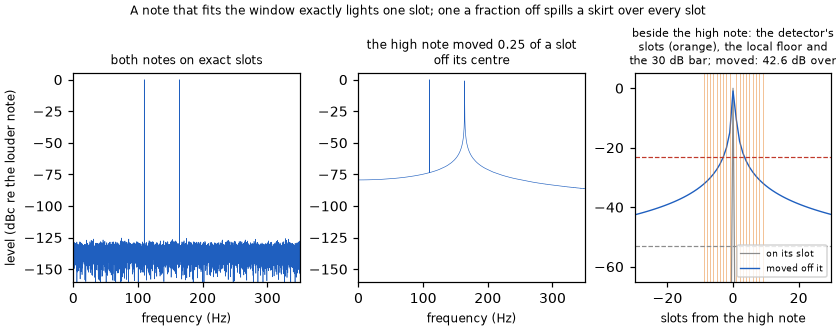
\includegraphics[width=0.98\linewidth]{explained-skirt.png}
  \caption{Two notes at the standard drive through a little noise, read
  through the analysis window the next chapter uses. Left: both notes on
  exact slots --- two lines and a flat floor. Middle: the high note moved a
  quarter of a slot off its centre, as the panel's title states; its skirt
  covers the whole span. Right: the slots either side of the high note in
  both cases, the nine the coherence check reads marked, with the local
  floor beside the note and the bar above it for the moved case.}
  \label{fig:skirt}
\end{figure}

The stretch is cut with a plain edge --- no fade at either end of the cut
--- which is what makes the exact-fit case perfectly clean and the
near-miss case spill. Many analyses soften the edges of their window to
blunt that spill, at the cost of blurring every slot into its
neighbours. The next chapter does not, because it can arrange for every
tone it cares about to fit exactly: it tunes the notes to the window
before it plays them. That arrangement is what the word \emph{coherent}
means there, and everything the chapter can do follows from it --- as
does the one thing it must check, which is that the notes really did stay
put.

\clearpage
\section{Chord IMD}
\label{sec:imd-plain}

\subsection{What this measurement tells you, and what it cannot}

Play two notes at once into a distortion pedal and more comes out than
the two notes and their harmonics. The circuit does not treat the notes
separately: it multiplies them together, and the output carries tones at
the sum of their frequencies, at the difference, and at every combination
of multiples of the two --- twice the low note less the high, three times
the high less twice the low, and so on. None of those tones is in either
note alone. This measurement --- the \term{two-tone} --- plays a musical
interval, a power chord's fifth by default, and lists every tone the pedal
invents from the pair.

Each invented tone is an \term{intermodulation-product}, named by the
recipe that makes it: so many of the low note plus or minus so many of
the high. Its \term{product-order} is how many multiples went into it ---
the sum-and-difference tones are order two, ``twice the low less the
high'' is order three --- and the app lists every recipe up to order
\imdMaxOrder{}, \imdRecipeCount{} of them on the standard probe. Each is
read at one slot of one long spectrum and quoted in \term{dbc}: decibels
below the louder of the two notes you played, so ``$-40$~dBc'' means a
hundredth of the note's size, whatever the volume was.

The record holds the level of every one of those recipes; the two notes
as the pedal delivered them; three percentage figures that earlier
versions of the app showed as tiles, kept for the record as those tiles'
frozen definitions; and the raw spectrum in the slots beside each played
note, kept for the check described later. Everything else --- what each
tone's reading is, how deep the recording could see, which musical job
each tone does, and how hard the pedal was driven --- is worked out
afresh from those stored facts every time the record is opened, so a
corrected rule corrects every record ever made.

\paragraph{What it cannot tell you.} Stated once.
\begin{enumerate}
  \item \textbf{Only one loudness.} One capture is one drive level, and
  a clipper's invented tones grow with drive faster than anything else
  about it. Two records are comparable only at the same drive, which is
  why the record states its drive on the page.
  \item \textbf{Whether a tone is the pedal's or the interface's.} An
  interface's converters invent tones of their own. A tone that stands
  above this recording's noise is real; the measurement does not say
  what made it. Only a capture with nothing in the loop --- a null run
  --- separates the two, and the floors described below neither do that
  job nor claim to.
  \item \textbf{Which stage moved the notes.} When the coherence check
  fails, the record says the notes did not stay still and stops there. A
  pedal with a dying battery moves a note as surely as an interface's
  clock does; the verdict has no culprit, by design.
  \item \textbf{Nothing below the recording's own floor} --- and, for the
  three old percentage figures, nothing about a floor at all: they are
  sums made at capture time over the tones that passed the presence test,
  and they carry no bound.
  \item \textbf{Nothing above order \imdMaxOrder{}.} The list of recipes
  is a small-signal census. A hard clipper driven into its bends has real
  energy at orders the list does not reach, so an empty row high in the
  list means measured and nothing found at this drive, never that the
  pedal makes nothing there.
  \item \textbf{Nothing about listening.} The chart says how much of each
  invented tone there is. It says nothing about what the distortion sounds like.
\end{enumerate}

\subsection{The test signal, and the lattice}

The signal is two sines of equal size played together, faded in over
\imdFadeMs{}~ms and out again at the end so that nothing bangs. The
standard loudness is \imdPeakDBFS{}~\term{dbfs} for the pair combined
--- each note \imdToneDBFS{}~dBFS on its own --- the same drive the other
measurements use, so that they all describe the pedal at one operating
point; the worked example later in the chapter uses the loudest drive the
hardware sheet offers, \tcCeilingDBFS{}~dBFS, where the reference
clippers actually clip. The default pair is \imdNoteOne{} and
\imdNoteTwo{}, a fifth on the low strings, named in ordinary equal
temperament (\imdNoteOneHz{}~Hz and \imdNoteTwoHz{}~Hz). The measure
sheet offers one kind of probe, the interval: you choose the two notes.

\paragraph{The premise, stated once.} Both notes are tuned, before
anything plays, so that each completes a whole number of cycles inside the
analysis window (Section~\ref{sec:slots-plain}). That is
\term{coherent-sampling}, and it has a consequence that makes the whole
measurement possible: slots add the way frequencies do. If the low note
sits on slot number $k_1$ and the high note on slot $k_2$, then ``twice
the low less the high'' sits on slot $2k_1 - k_2$ --- exactly, not
approximately --- and so does every other recipe, on its own slot,
leaking into no neighbour. The set of slots the two notes and all their
invented tones occupy is the \term{analysis-lattice}, and the analyzer
reads each recipe at its one slot and nowhere else.

\paragraph{Two numbers describe the lattice.} Write the two slot numbers
as a common factor times a simplest fraction --- the low note's slot is
$g$ times $a$, the high note's $g$ times $b$, with $a$ and $b$ sharing no
factor. The two parts answer two different questions.

The fraction $a : b$ is the \term{reduced-ratio}, and it decides whether
two different recipes can ever land on the \emph{same} slot. They can only
when the two numbers are small: for recipes up to order \imdMaxOrder{}, a
fraction whose two numbers add to \imdMinimumReducedSum{} or more keeps
every recipe on its own slot, and the bound is exact --- the fraction
\imdCollidingRatio{}, whose numbers add to \imdCollidingSum{}, still has a
collision, and every fraction one higher is clean. The common factor $g$
is the \term{lattice-spacing}, and it decides how \emph{close} two
invented tones can get: every recipe's slot is a whole multiple of $g$, so
no invented tone can sit nearer than $g$ slots to another, or to either
played note. A lattice can pass the first test and fail the second. The
probe the app used until its window was lengthened shared no slots and
still put four recipes two slots from the played notes, where a note's own
skirt lives; the records made on it carry that mark, as a later section
explains.

That is also why a consonant interval is an awkward one to measure. A
fifth is, in its simplest form, a ratio of three to two, and
three-to-two is a fraction with tiny numbers --- the most crowded lattice
there is, with recipes landing on top of each other and on the notes
themselves. The measurement has to move the notes off that exact ratio,
and the question is how far, and in which direction.

\paragraph{The snap.} The \term{lattice-snap} is done in two steps, so
that the interval you ask for is one interval at every sample rate.
First, the fraction is chosen \emph{once}, against every sample rate the
app offers at the same time: no two recipes may share a slot; every recipe
must sit at least \imdResolvableSpacing{} slots from the played notes at
every rate; both notes must stay within \imdCentsBudget{}~cents of the
pitch you asked for; and among the fractions that manage all three
(\imdSurvivorCount{} do, for the fifth), the one whose interval is nearest
the one you asked for wins. The default fifth lands on
\imdRatioA{}~:~\imdRatioB{} --- an interval of
\imdStandardIntervalCents{}~cents against the \imdRequestedIntervalCents{}
of equal temperament, \imdIntervalFlatCents{}~cents flat, and the same at
every rate. Second, on the rate at hand, that fraction is scaled up by
whatever common factor fits the slot grid: at \imdClassARates{} the
notes land on slots \imdClassABinOne{} and \imdClassABinTwo{}, spaced
\imdClassASpacing{} apart, with the low note \imdClassACentsOne{}~cents
and the high \imdClassACentsTwo{}~cents from equal temperament; at
\imdClassBRates{} on slots \imdClassBBinOne{} and \imdClassBBinTwo{},
spaced \imdClassBSpacing{}, at \imdClassBCentsOne{} and
\imdClassBCentsTwo{}~cents. The interval tile on every record prints the
offsets that capture was played at. Keeping the interval outranks
everything else: a window too short to place the fraction at a good
spacing --- Simulation Mode's quick preview --- still asks the same
musical question, and the reading rules carry the crowding honestly.

Some pairs the app refuses. If a requested interval cannot escape an exact
small fraction within the cents budget at all, the plan stops before
anything plays and says which lattice it found and why it fails. It never
falls back to the naive tuning, because on an exactly degenerate lattice
several recipes share each slot, the enumeration keeps one label per slot
by a tie-break, and the record would come out looking cleaner than the
pedal is --- a table whose labels are not facts.

\paragraph{The window is a duration.} The analysis window is
\imdStandardLength{} samples at \imdStandardRateKHz{}~kHz --- two to the
power \imdStandardLengthPower{}, about \imdWindowS{}~s of steady tone,
with slots \imdBinWidthHz{}~Hz apart. What that fixes is the
\emph{duration}, not the sample count: at each of the other rates the app
takes the power of two nearest the same length of time, so the
\imdSupportedRatesKHz{}~kHz rates form two pairs that share a slot grid.
The two-tone signal is then made long enough to hold the window, plus the
fades and a short settle at each end --- \imdStimulusClassAS{}~s at
\imdClassARates{}, \imdStimulusClassBS{}~s at \imdClassBRates{} --- never
set by hand. That rule exists because of a mistake it corrected. An
earlier version fixed the window as a sample count and set the signal's
length by hand, and at two of the four rates the window ran into the
fade-out: the notes no longer fitted the window, their skirts flooded the
low slots, and the deepest products could not be told from the window's
own leakage. Figure~\ref{fig:imd-window} shows the window inside the
signal as the app now sizes it, and the old case beneath it.
Figure~\ref{fig:imd-lattice} shows the lattice itself: every recipe as a
stem at its slot and order on the shipped fifth, the same on the old
crowded probe with its four recipes beside the notes in red, and a close
look at the slots beside the low note.

\begin{figure}[htbp]
  \centering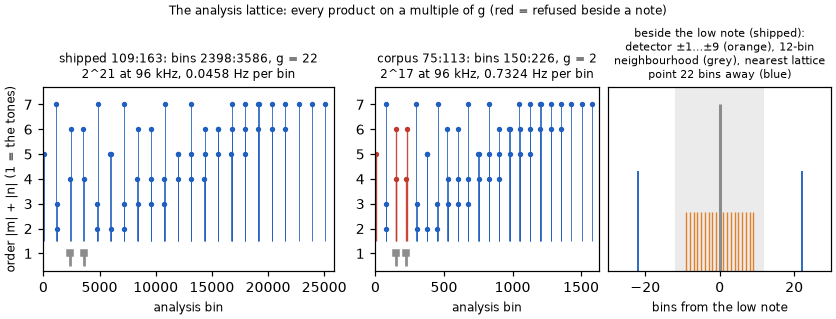
\includegraphics[width=0.95\linewidth]{imd-lattice.png}
  \caption{The analysis lattice. Left: every recipe as a stem at its slot
  and order on the shipped fifth, the two played notes as squares at order
  one; every stem sits on a multiple of the spacing. Middle: the same on
  the crowded probe every earlier record was made on --- the four recipes
  two slots from the notes and the one two slots from zero are red,
  refused on position. Right: the slots beside the low note on the shipped
  lattice --- the nine the coherence check reads, the neighbourhood the
  reading rule guards, and the nearest recipe a spacing away.}
  \label{fig:imd-lattice}
\end{figure}

\begin{figure}[htbp]
  \centering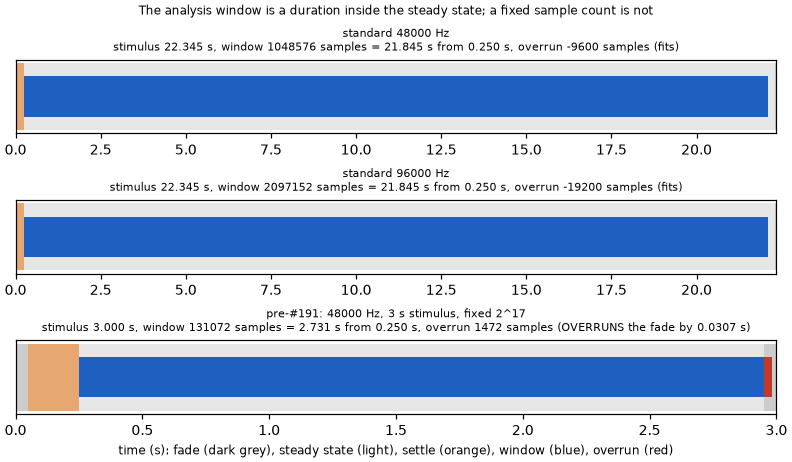
\includegraphics[width=0.95\linewidth]{imd-window.png}
  \caption{The analysis window inside the two-tone signal at two rates as
  the app now sizes it (top two), and the earlier fixed-length window on a
  hand-set signal, which ran into the fade-out (bottom, the overrun in
  red).}
  \label{fig:imd-window}
\end{figure}

\subsection{How the answer is read}

Eight steps, each in words; the technical reference gives the exact rule
for each.

\paragraph{The window.} The app measures the delay through the rig on
every capture and lines the recording up with the signal. The window then
starts after the fade-in and the settle and runs for exactly its length;
the moment the fade-out begins is the end of the steady state, and the
signal is sized so that the window ends before it. The analyzer never
shortens a window it is handed: the notes were tuned to fit that length,
and a shorter cut would spill far worse than the fade it avoided.

\paragraph{The spectrum.} One long transform over the window, cut with
plain edges and no taper (Section~\ref{sec:slots-plain}), scaled so that
a note which fits exactly reads as its own size.

\paragraph{The walk.} Starting with the two notes' slots and slot zero
already claimed, the analyzer walks every recipe from order two up to
order \imdMaxOrder{}, in order, and admits each one whose frequency lies
between one slot's width and just under half the sample rate --- unless
its slot is already taken, in which case the recipe is dropped. So where
a crowded lattice puts two recipes on one slot, the lower order keeps it,
and on the shipped fifth, where nothing collides, exactly
\imdRecipeCount{} recipes are admitted. The whole lattice is collected
before any noise is measured, so that the noise can be measured away from
it.

\paragraph{The reads.} Each recipe's size is the value of its one slot,
exactly; so are the two notes'. An earlier version took the largest of
the slot and its two neighbours, ``to tolerate drift'' there was none of.
That left a strong tone untouched and lifted every reading at the noise by
about \imdOlderReadBiasDB{}~dB on average; records made that way still
carry those reads, and their floor was measured the same way, so their
margins stand.

\paragraph{The local floor, and the gate.} Each invented tone is judged
against the noise measured right beside it: the \term{local-floor} is the
middle value of the slots from \imdLocalFloorInnerBins{} out to about
\imdLocalFloorSpanHz{}~Hz out on either side (\imdLocalFloorOuterBins{}
slots at the standard rate, and never fewer than
\imdLocalFloorMinimumOffsets{}), with every slot the lattice claims cut
out by name --- every other recipe, both notes, slot zero, and the
detector's slots beside each note described below. The three nearest
slots are left out because they are the tone's own: if coherence is ever
lost, a skirt lands there first, and a floor must never be read from the
skirt of the thing it judges. The span is held in hertz rather than in
slots because noise is local in frequency, and a fixed slot count would
have shrunk sixteenfold when the window grew. The \term{gate} is then a
fixed bar: a tone counts as \emph{present} when it stands more than
\imdGateFactor{} times (\imdGateDB{}~dB) above its local floor. That
verdict is decided once, at capture, and written into the record;
nothing decided later can change it. The right-hand panel of
Figure~\ref{fig:imd-spectrum} is the picture: the grey span either side
of one recipe, the lattice slots cut out of it in red, the floor through
the middle and the gate four times above it.

\paragraph{The three percentages.} Over the invented tones inside the
audible band (\imdAudibleLowHz{}~Hz to \imdAudibleHighHz{}~Hz) the
analyzer adds up three sums as percentages of the notes: two borrowed
from laboratory two-tone standards, and one over every tone that passed
the gate. They were the tiles of earlier builds and survive as those
tiles' frozen definitions; the roles described later replaced them.

\paragraph{The detector.} For each played note the analyzer keeps the raw
spectrum at the \imdDetectorMaxOffset{} slots either side of it, and the
local floor beside that note, in the record: the \term{coherence-detector}.
Nothing else keeps those slots, and they are what the coherence check
reads.

\paragraph{What is stored.} The invented tones, loudest first, each with
its recipe, frequency, size, order and gate verdict; the signal as
delivered; the two notes' sizes; the three sums; the band; and the
detector. Nothing worked out at reading time is stored.

\subsection{What the app decides when it reads a record back}

Everything in this section is computed from the stored record every time
it is opened. A reader that knows the window's length says so; one that
does not places nothing on the lattice and makes the smaller claim.

\paragraph{The capture floor.} The record states how deep this
particular recording could see: the \term{capture-floor}. It is the
middle value of the levels of every recipe the gate did \emph{not} pass
--- leaving out any the rules below refuse for a reason of their own: a
recipe inside a note's skirt, one under the band's low edge, one beside a
louder tone --- with at least \imdMinimumFloorSamples{} such empty slots
needed, and fewer than that honestly reported as no floor. Slots that lie
under the loudest tone's own skirt deliberately stay in, because on a
record like a rectifier's every empty slot is under it, and a vanished
floor would read as ``every tone resolved''. The two floors run one way:
the gate is decided at capture against the raw spectrum, the capture floor
is a summary made afterwards over slots already judged, so leaving a
refused slot out of the floor changes which judged slots are averaged and
never which slots were judged.

\paragraph{One reading per tone.} Every invented tone gets one
\term{product-reading}, and the app prints four kinds of answer: measured;
nothing found down to a stated level; could not be read, and why; and out
of band. The rules are applied in a fixed order, stopping at the first
that fits, and position comes before level throughout.
\begin{itemize}
  \item \textbf{Beside a played note, or beside zero} --- within
  \imdNeighbourhoodBins{} slots of either note's slot or of slot zero:
  could not be read. A slot that close holds the note's own skirt, and a
  slot beside zero holds the recording's own offset and slow drift. This
  is decided on position alone, before any level is looked at, because
  the gate samples its floor from slots that lie mostly outside the skirt
  the slot is sitting in and would pass such a slot with a confident
  margin.
  \item \textbf{Under the band's low edge} --- below \imdAudibleLowHz{}~Hz:
  out of band. A fact about frequency, not a limit of the instrument, so
  its sentence never merges with a lattice's or the analyzer's. On the
  shipped fifth one recipe lands there: \imdSubBandRecipe{}, about
  \imdSubBandHz{}~Hz up, where nothing a pedal does can be told from the
  recording's own drift.
  \item \textbf{Beside a louder invented tone} --- within the same
  \imdNeighbourhoodBins{} slots of a louder tone that itself passed the
  gate: could not be read. At that separation the quieter slot holds the
  louder tone's skirt. The louder of the pair is read; the quieter is not.
  A neighbour that is only noise casts no skirt and refuses nothing. On
  the shipped fifth nothing is ever closer than \imdClassASpacing{} slots,
  so this rule marks nothing; on the old crowded probe it marks many.
  \item \textbf{Inside the analyzer's own leakage} --- on an old record
  whose window ran into the fade-out, a tone too deep below the loudest
  component to be separated from the window's skirt: could not be read.
  No record the app makes now gets this one.
  \item \textbf{Under the loudest tone's skirt} --- on a record whose
  loudest invented tone stands above the played notes and whose
  coherence check could not be read, a tone deeper below that loudest
  one than a skirt reaches at the lattice spacing
  (\imdClassASkirtDepthDB{}~dB at \imdClassASpacing{} slots): unread,
  never present and never absent.
  \item \textbf{The gate passed} --- measured, with its margin over the
  capture floor when there is one.
  \item \textbf{No floor to read against} --- could not be read, carrying
  the count of empty slots it had.
  \item \textbf{Otherwise} --- nothing found down to the slot's own level:
  a bound, never a value, and never a rank.
\end{itemize}
A refusal is never quietly filed as ``absent'', and ``absent'' is never
a number. The record counts the four kinds and states its floor by its
reason: a floor, or ``every tone resolved'' only when nothing was
refused, or ``too few empty slots'' with the counts.

\paragraph{Shared slots, and the second-order cross-check.} On a record
made on an exact small fraction --- the original fifth, an exact three to
two --- several recipes share a slot, and the label the record shows is
the walk's tie-break. Such a record marks those rows as shared, from the
stored notes alone, and the cross-check leaves them out. The cross-check
itself is a fact about second-order tones: a single squared term makes
the sum and the difference of the notes at equal size, and twice each
note at sizes that differ by twice the notes' own gap in the output, so a
tone standing more than \imdPartnerToleranceDB{}~dB above what its
partner licenses is not a clean second-order reading --- the slot holds
something else too, and its label and rank are not to be trusted. Only
excess flags; the quieter partner stays trustworthy.

\paragraph{The coherence check.} This is the section the reader most
needs, because everything above rests on one premise, and the premise
has no margin.

\emph{What ``coherent'' means here.} The window is cut with plain edges,
so a note that fits it exactly is perfectly clean and a note that does
not spills a skirt over every slot (Section~\ref{sec:slots-plain}). The
notes were tuned to fit. But the tuning is a fact about the signal the
app sent; whether the notes \emph{stayed} on their slots for the whole
window is a fact about the chain, and anything in it that drifts during
the capture --- an interface clock, a sagging supply, a circuit warming
up --- breaks the fit. When it breaks it does not degrade gently: the
note's skirt lands across the whole lattice and buries the invented
tones, and every level on the record, floor included, is a reading of the
skirt.

\emph{Where to look.} The spill lands first and hardest in the slots
immediately beside each note, so those are the slots the
\term{coherence-check} reads: the \imdDetectorMaxOffset{} either side of
each note, kept in the record by the detector. Every one of the nine is
read, not only the odd ones, and that is a measured fact rather than a
choice: a note that wobbles an even number of times across the window
puts its spill in the even slots only, and a detector that read the odd
ones alone saw a clean floor on the very capture whose stored recipes two
slots from the notes read far above it.

\emph{The floor and the bar.} The worst of those slots is compared with
the local floor measured beside that same note, and the excess is read
against a bar of \imdBarDB{}~dB over it. The bar is relative to the floor,
not an absolute level, because a spilled note's energy does not shrink
when the slots get finer while noise does; an absolute bar was right at
one window length only. Beside the excess the record prints what noise
alone would put the worst of that many slots over the floor --- about
\imdNoiseExcessDetectorDB{}~dB for the \imdDetectorBinCount{} slots the
detector reads, about \imdNoiseExcessLegacyDB{}~dB for the
\imdLegacyBinCount{} that older records offer --- a reference so that a
reading over four slots and one over thirty-six can be laid side by side,
never a bar.

\emph{Distance is only a stand-in for level.} Being far from every
invented tone is necessary and not enough. Under lost coherence a tone
spills a skirt too, and a slot beside a note reads the note's skirt only
while the loudest invented tone, sitting a spacing away on the other side,
is quiet enough for its skirt to sit under the note's there by a stated
margin (\imdProductSkirtMarginDB{}~dB). That gives each slot a ceiling on
how loud the loudest invented tone may be: the nearest slot tolerates one
up to \imdCeilingNearestDBc{}~dBc, louder than the notes themselves, and
the ninth only one below \imdCeilingWidestDBc{}~dBc, so the nearest slots
are the last to survive. The check reads only the slots whose ceiling the
record's loudest tone clears. A device whose invented tones stand above
its own notes --- a full-wave rectifier does this --- clears no ceiling,
and then the check reads nothing and the line says why: the slots beside
the notes would be reading the products' coherence, not the notes'.

\emph{What the verdict is, and is not.} When the check reads and the
excess is over the bar, the record says the played notes did not stay
stationary across the window, from some source in the chain that the
reading cannot name, so this capture's floor and every invented tone's
level are not trustworthy. Nothing is refused, discarded or re-run: the
capture is saved as measured with that sentence on it, and the measure
sheet announces it the moment the number exists. The sentence never
names a stage --- a pedal with a dying battery moves a note over twenty
seconds as surely as a rig --- and it is a statement about this capture,
not about the pedal. Under the bar it says the premise held.

\emph{A shape, never a verdict.} The record also quotes the
\term{pair-statistic}: the average of the two innermost slots beside each
note, and the difference between the high note's pair and the low
note's. A shared wander in frequency puts the high note's pair above the
low note's by a fixed amount the record prints beside it; a wobble in
level, or a wobble in timing that treats both notes alike, leaves the two
pairs equal. The line states the numbers and draws nothing from them,
because equal pairs are consistent with two different causes and the
shape has not earned a verdict. Figure~\ref{fig:imd-detector} shows the
detector's slots on a clean loop and on the pipeline's wander fixture,
and the ceilings.

\begin{figure}[htbp]
  \centering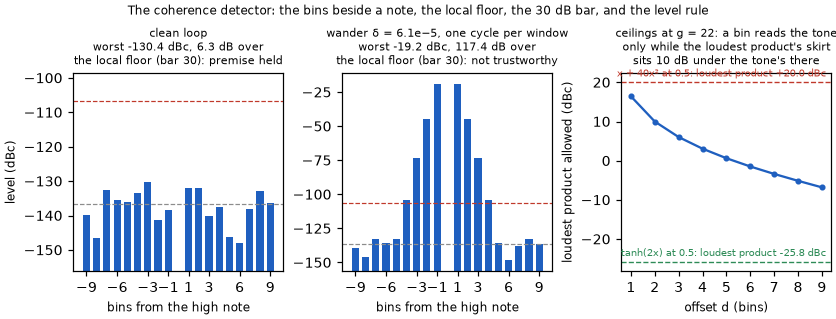
\includegraphics[width=0.95\linewidth]{imd-detector.png}
  \caption{The coherence check. Left: the nine slots either side of the
  high note on a clean loop through a little noise, with the local floor
  beside the note (grey) and the bar above it (red) --- within a few
  decibels of the floor, premise held. Middle: the same slots on the
  pipeline's wander fixture, a shared drift of both notes at one cycle
  per window --- far over the bar, not trustworthy. Right: the ceiling
  each slot sets on the loudest invented tone at the shipped spacing, with
  the worked example's loudest tone far below every ceiling and a squarer
  driven above its own notes clearing none.}
  \label{fig:imd-detector}
\end{figure}

\paragraph{The harmonic roles.} The tiles at the top of the record sort
the invented tones by what each does to the chord you \emph{asked for}.
That last phrase is the point. To keep the tones separable the app moved
the notes a few cents onto the lattice, so a sorter that read the lattice's
own frequencies would call the octave below the root ``twenty cents
flat'' when it is exactly the chord tone the lattice displaced. So the
roles are classified at the interval you requested and measured at the
lattice: the \term{harmonic-role} is decided from the recipe alone, and
the level is read from the slot the tone actually landed on.

The request is not written on the record, so the app recovers the two
notes as the nearest equal-tempered pitches to the delivered tones, which
is unambiguous inside the cents budget --- the one place the delivered
frequencies are consulted, and only to name the notes. It then takes the
interval's \term{just-ratio}: the simplest whole-number fraction, using
only the factors two, three and five, within \imdPitchToleranceCents{}
cents of the equal-tempered interval --- \imdFifthJustRatio{} for the
fifth, so the grid is built on the note a fifth's ratio implies, a
fundamental of \imdFifthGridHz{}~Hz for \imdNoteOne{} and
\imdNoteTwo{} --- and it lays a grid of multiples of that fundamental.
Every recipe lands on that grid at a whole-number step, exactly, and its
pitch class is read off by octave reduction: halve or double the step
until it sits inside one octave above the root, then ask which note that
is and how far from it. Figure~\ref{fig:imd-roles} shows where each of
the \imdRecipeCount{} recipes lands on the fifth's grid, coloured by the
role assigned to the step; the role table in the technical reference
lists each step's pitch and role.

The five roles, named as the app names them. \textbf{Thickening}: a tone
on a played note's pitch class, at or above the low note --- it reinforces
the chord. \textbf{Growl (sub-octave)}: the same pitch classes, below the
low note --- weight under the chord. \textbf{Added colour}: a tone on a
pitch that is not a chord tone but is in tune with the chord
(\imdAddedColourNames{} above the root). \textbf{Sourness (clash)}:
everything else --- any other pitch class, and any step that lands more
than \imdPitchToleranceCents{} cents from every fret. \textbf{All
products}: the total, how much rather than what kind. The tolerance is
not chosen: the widest gap between a just interval built from those three
factors and its equal-tempered fret is under it, and the nearest point a
two-tone grid can produce from a larger factor is beyond it, so the bar
sits in an empty band. A role's figure is the power sum, in dBc, of the
measured tones in it, counting each slot once; a tone the app found
nothing for adds nothing and is bounded by the record's floor; a tone the
app could not read was never looked at, so a role that holds one is
marked as a lower bound, and the line under the tiles names the recipes
left out. The record also states what it enumerated --- the recipe count
and the orders --- so a tone missing from the list can be told from one
that was measured and silent.

\begin{figure}[htbp]
  \centering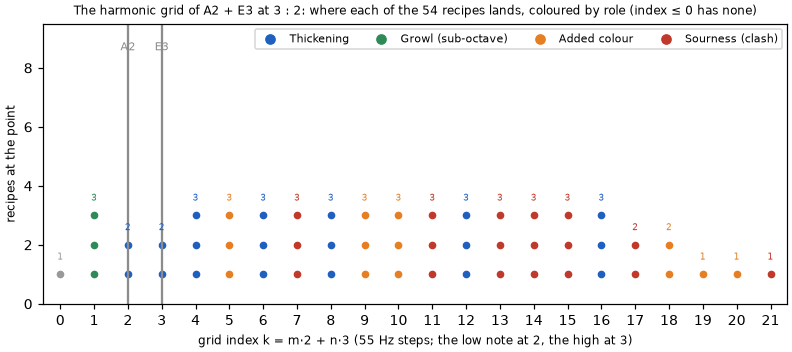
\includegraphics[width=0.95\linewidth]{imd-roles.png}
  \caption{The harmonic grid of the requested fifth at its just ratio:
  every recipe at its grid step, stacked where several share a step and
  coloured by the role assigned to that step; the two played notes
  marked. Step zero and below has no role.}
  \label{fig:imd-roles}
\end{figure}

\paragraph{The drive line.} The record states how hard the pedal was
driven, read from the stored signal: the two notes' combined peak and
each note's own level in dBFS, in volts at the pedal input as well when
the record's own calibration measured the interface, and a note that the
two tones are equal --- every order relation above assumes it.

\subsection{The settings}

Every setting is in the technical reference's Chord IMD chapter, in three
tables read from the manifest: the parameters, the lattice the app
chooses on every sample rate, and the role grid of the default fifth.
This chapter repeats only the handful a reader acts on. The default pair
is \imdNoteOne{} and \imdNoteTwo{}, delivered \imdClassACentsOne{} and
\imdClassACentsTwo{}~cents from equal temperament at \imdClassARates{}
(\imdClassBCentsOne{} and \imdClassBCentsTwo{} at \imdClassBRates{}),
within a budget of \imdCentsBudget{}~cents; the window is about
\imdWindowS{}~s and the signal \imdStimulusClassAS{}~s or
\imdStimulusClassBS{}~s long; the walk covers \imdRecipeCount{} recipes
up to order \imdMaxOrder{}; a tone is present at \imdGateFactor{} times
its local floor; the coherence bar is \imdBarDB{}~dB over the floor; and
a grid step counts as on a fret within \imdPitchToleranceCents{}~cents.

\subsection{What the result looks like}

Figure~\ref{fig:imd-spectrum} is the worked example --- the soft clipper
of the earlier chapters, at the loudest hardware drive, on the shipped
fifth through a little noise --- as the pipeline reads it. On the left is
the whole spectrum below the notes' first few multiples: every recipe
marked measured (blue), nothing found (grey) or refused (red), the two
notes as squares at zero, and the capture floor as the dashed rule with
its slot count. The clipper is symmetric, so every even-order recipe
reads at the floor and every odd-order one stands well above it, in a
ladder that falls away with order. On the right is the local-floor
neighbourhood of one recipe: the grey span either side of it, every
lattice slot cut out of it in red, the floor as the middle value of what
remains, and the gate four times above it.

\begin{figure}[htbp]
  \centering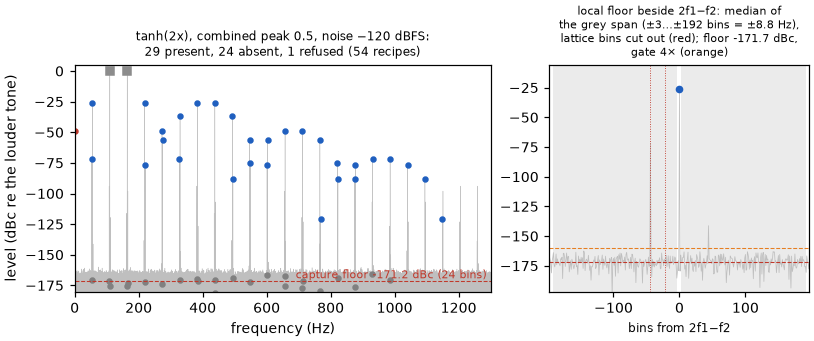
\includegraphics[width=0.95\linewidth]{imd-spectrum.png}
  \caption{The worked example, a soft clipper at the loudest hardware
  drive on the shipped fifth through seeded noise. Left: the spectrum with
  every recipe marked measured (blue), nothing found (grey) or refused
  (red), the two notes as squares, and the capture floor as the dashed
  rule. Right: the local-floor neighbourhood of one recipe, with the
  lattice slots cut out (red), the floor (red, dashed) and the gate
  (orange, dashed).}
  \label{fig:imd-spectrum}
\end{figure}

The app's own chart, rendered from its chart code on its simulated pedal
(never a screenshot), is Figure~\ref{fig:app-imd}. Across the top run the
tiles: the interval played, with the cents each note was moved and the
frequencies delivered; then the five roles, each with its figure in dBc
and a one-line gloss. Under them, lines state the recipe count and orders
enumerated, that the roles are assigned at the requested interval and the
levels read at the lattice, and the drive level. The chart itself sits on
a musical pitch axis, labelled with note names and their frequencies:
the two played notes in one colour and every invented tone as a stem in
one of two others, one for the even orders and one for the odd, with the
legend saying that a dotted stem is not a reading and a faint one was
read against the floor and not ranked. Below the chart the invented tones
are ranked loudest first, each with its recipe, the pitch it lands on and
its deviation in cents, its frequency, its level in dBc, its margin over
the floor, and its order; under the table, one line names the recipe
under the band, one gives the floor --- or says why there is none --- and
one is the coherence check, quoting the worst slot, its excess over the
floor beside the note, what noise alone would put there, its distance from
the bar, and the pair statistic.

\begin{figure}[htbp]
  \centering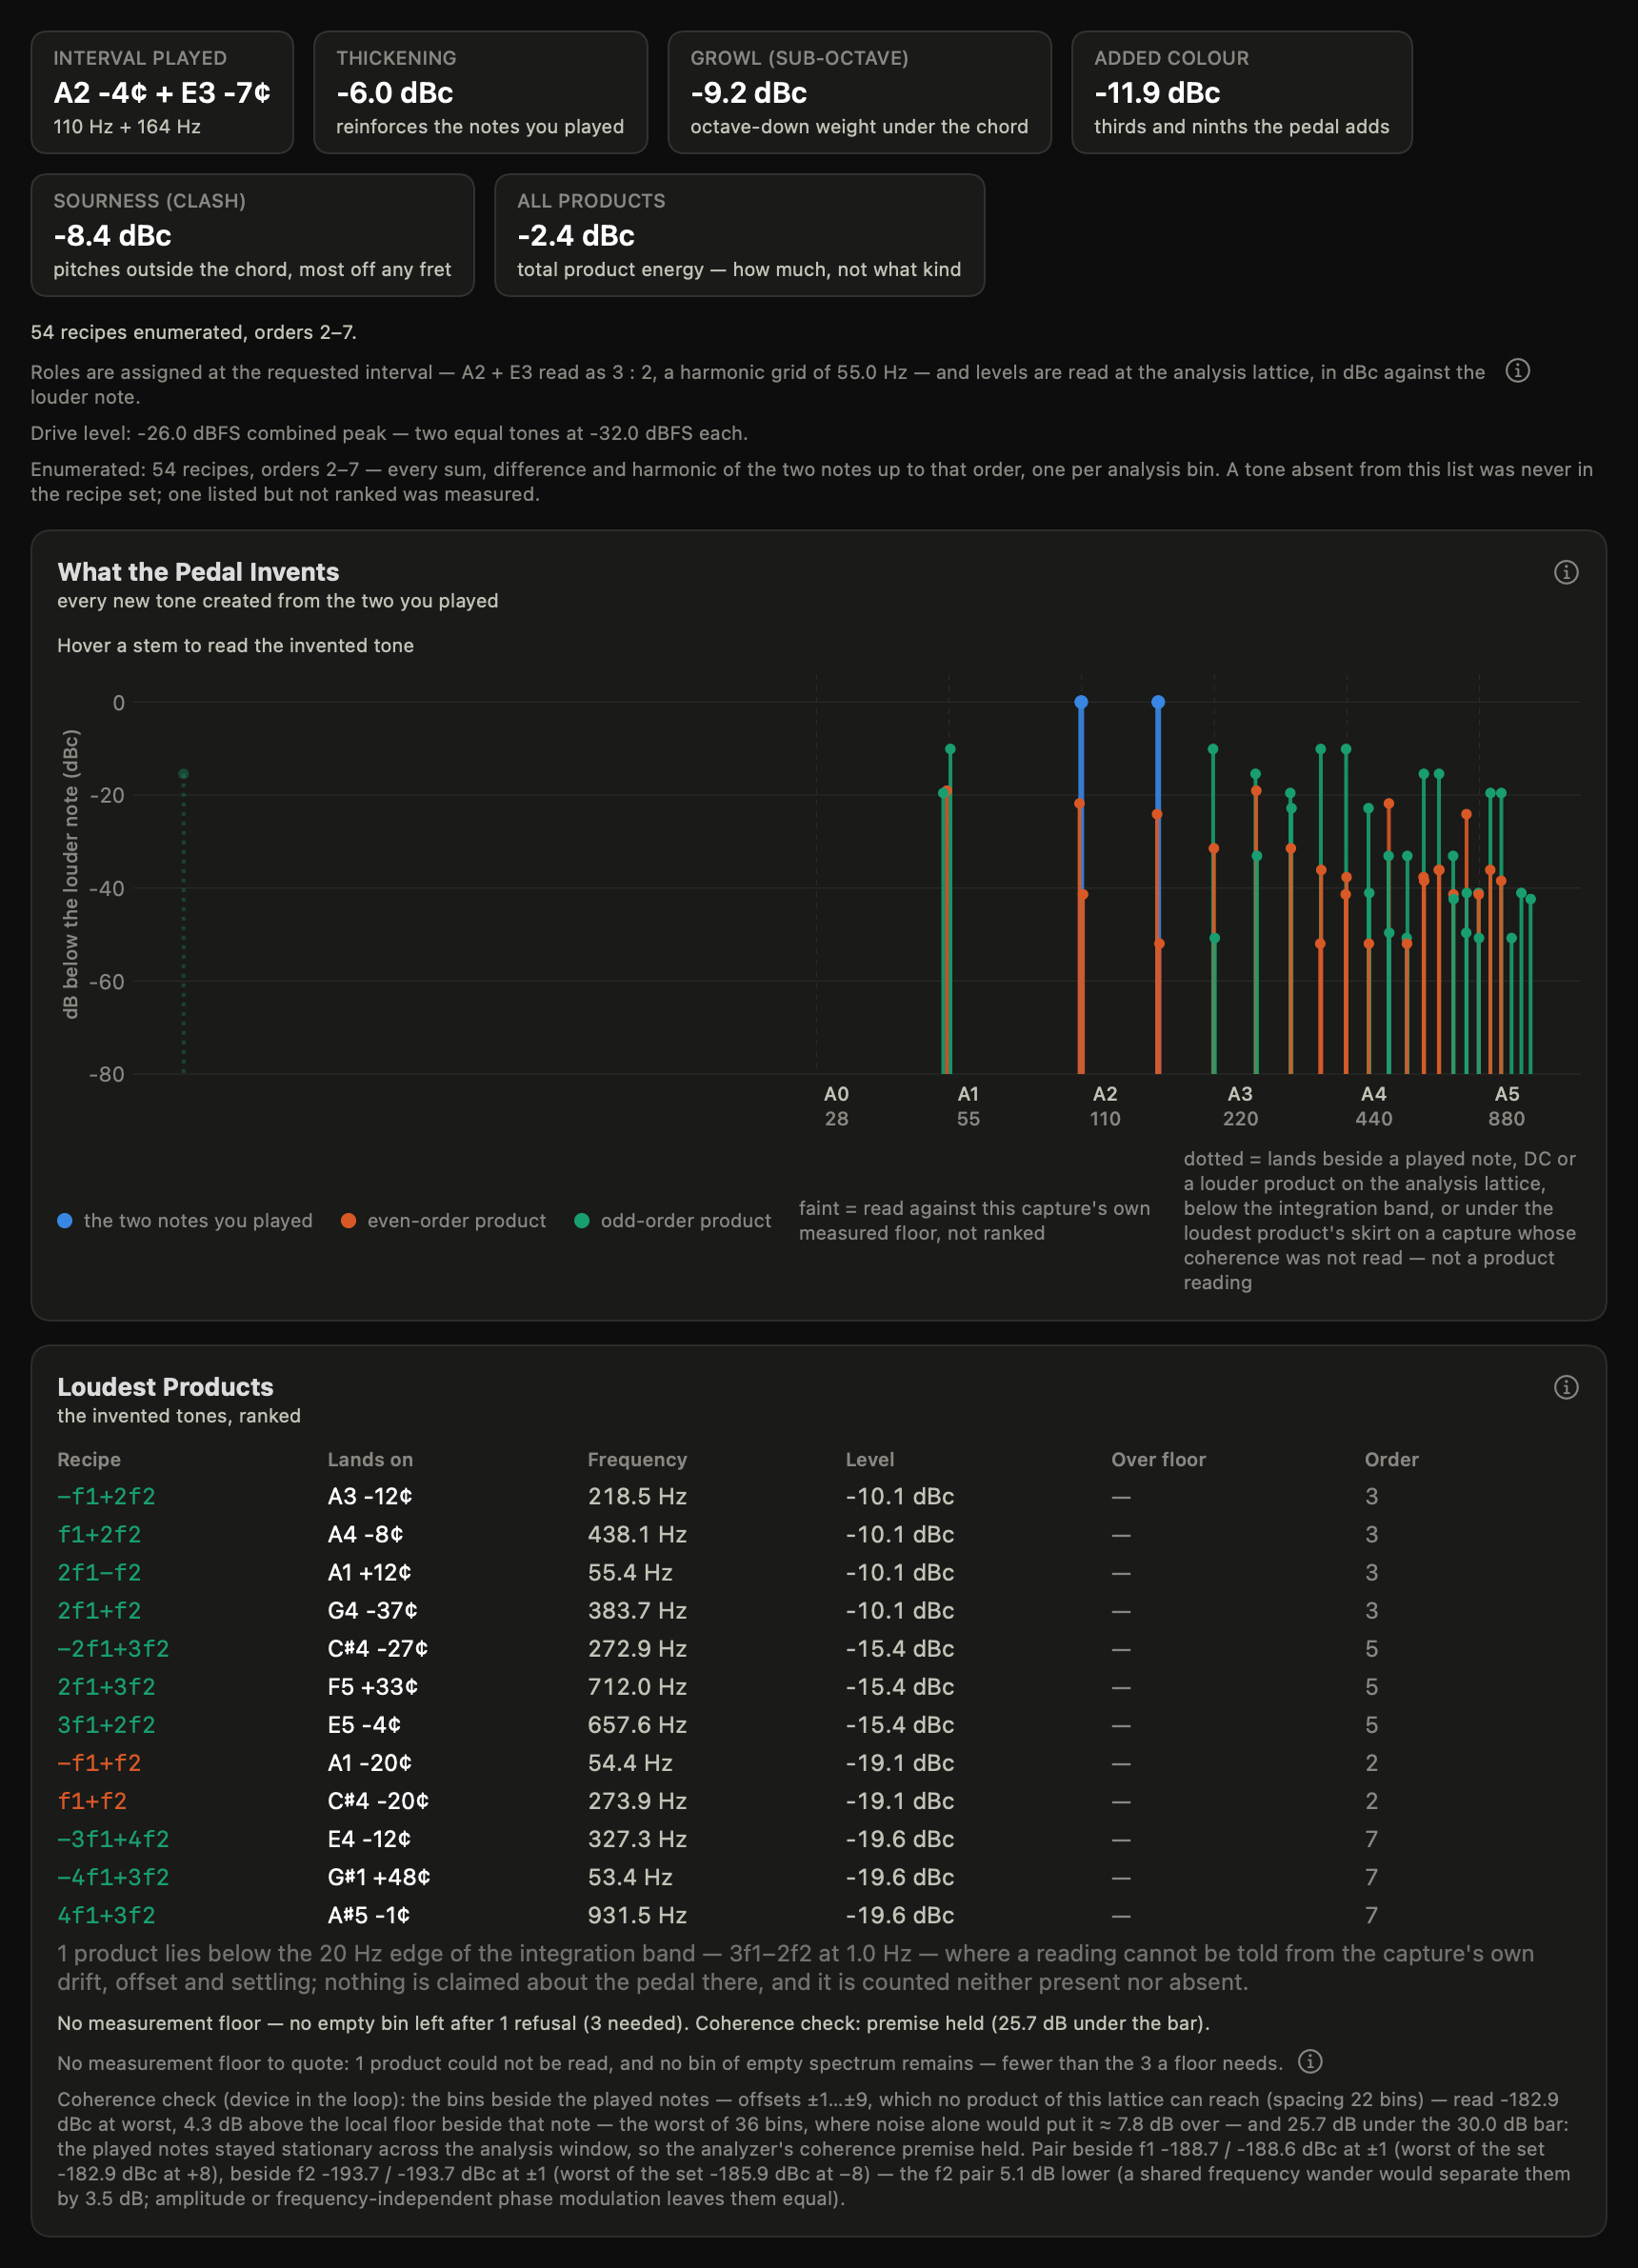
\includegraphics[width=0.85\linewidth]{chord-roughness--sim-power-chord.png}
  \caption{The Chord Roughness view as the app draws it, for its simulated
  pedal fed the default fifth at the standard drive.}
  \label{fig:app-imd}
\end{figure}

\subsection{How you can check that the app does what this says}

As in the earlier chapters, a second program was written from the
description --- in Python, independently, not by translating the app's
code --- and the \term{parity} runs both on the same made-up devices and
demands the same answer. It runs \iparityCaseCount{} cases, and each
device case a second time as its \term{phantom} twin
(\iparityTwinCount{} twins), on the signal the app's own tuning produces,
so the choice of lattice is exercised rather than assumed.

The known answer deserves a paragraph of its own here, because it is
what makes the check strong. For a device with no memory --- one whose
output at each instant depends only on its input at that instant --- two
notes on exact slots produce an output that repeats along two directions
at once: advance the low note by one cycle and the output repeats, advance
the high note by one cycle and it repeats again. A signal that repeats on
a grid like that is made of exactly the recipes the chapter lists, and
each recipe's size is a definite number that can be computed by
integrating the device's formula over one cycle of each note. The second
program does that integration for every case and prints the exact size
beside the app's reading of it; for the formula devices it also works the
size out a second way, by expanding the formula, and holds the two
methods to each other.

The case families, in a sentence each. The lattice alone, at every sample
rate and both short windows, for the fifth, an octave, a major third and
a pair that must be refused. Three formula devices --- a gentle curve, a
plain squarer and a lopsided clipper --- and the soft and hard clippers of
the earlier chapters, all at the loudest hardware drive. A phantom that
plants every one of the \imdRecipeCount{} recipes at a ladder of sizes.
A plain wire through noise, at two levels and two window lengths. A
squarer behind a tone filter and the soft clipper with a filter before
it. The old crowded lattice with a squarer and a cubic. The wander
fixture, read the old way and through the detector. A squarer driven
until its invented tones stand above the notes. And the worked example
analyzed \iparityLatencySamples{} samples late.

The demands, in numbers the pipeline writes into this document. The two
programs must agree on every level to within \iparitySwiftWords{} of a
decibel (\iparitySwift{}~dB) on a capture with no filter in it --- on the
run that built this document the worst disagreement was
\iparityWorstSwiftWords{} (\iparityWorstSwift{}~dB) --- and within
\iparitySwiftFilteredWords{} (\iparitySwiftFiltered{}~dB) through a
filter, whose arithmetic rounds differently in the two languages over
two million samples (measured \iparityWorstSwiftFilteredWords{},
\iparityWorstSwiftFiltered{}); every yes-or-no reading --- slot, gate,
reading and its reason, grid step, role, shared-slot mark, cross-check
--- must be identical, and every sentence the record prints identical.
The two exact answers must agree with each other to
\iparityTruthRelativeWords{} of their size (\iparityTruthRelative{}),
and the expanded formula with the integration to \iparityClosedFormWords{}
(\iparityClosedForm{}). Every recipe that a device cannot produce must
read at or below \iparityEmptyDepth{}~dBc on a noiseless capture (worst
measured \iparityWorstEmpty{}) --- the depth at which nothing can be told
from the loudest tone is set by the arithmetic's precision, not by the
window. The app's reading of every recipe a device does produce must
match the exact answer, once the noise in the slot is allowed for, within
\iparityTruthBandlimitedWords{} of a decibel (\iparityTruthBandlimited{})
for the smooth devices, within \iparityTruthKinkedWords{}
(\iparityTruthKinked{}) for the two with a kink in them, and within
\iparityTruthPhantomWords{} (\iparityTruthPhantom{}) on every phantom.
The lattice each case played must be the one the manifest recorded by
running the app's tuning on that grid, field for field, and the refused
pair refused with the same numbers on both sides. The wire through noise
must read every recipe as nothing found, with its capture floor within
\iparityFloor{}~dB of the value the noise's own statistics predict
(measured \iparityFloorLongDeficitWords{} and
\iparityFloorShortDeficitWords{} of a decibel short at the two lengths,
\iparityFloorLongDeficit{} and \iparityFloorShortDeficit{}) and its
coherence excess within \iparityCoherenceNoise{}~dB of what noise alone
puts over the floor (measured \iparityCleanExcess{} against
\iparityCleanExpected{}). And the late analysis must move the window by
exactly its offset, keep the same overrun, and move no recipe's level by
more than \iparityLatencyToleranceWords{} of a decibel
(\iparityLatencyTolerance{}; measured \iparityWorstLatencyShiftWords{},
\iparityWorstLatencyShift{}). \iparityPartBStatus

Two of those results are worth stating in words. The two devices with a
kink in them --- the hard clipper, and the lopsided one --- are applied to
the signal sample by sample, so what they make above half the sample
rate folds back down, and on a two-tone lattice a folded tone lands
\emph{exactly} on a low-order slot: \iparityHardclipAliasWords{} of a
decibel (\iparityHardclipAlias{}) at \iparityHardclipAliasAt{} and
\iparityAsymAliasWords{} (\iparityAsymAlias{}) at \iparityAsymAliasAt{},
against \iparityHardclipTwinWords{} and \iparityAsymTwinWords{} on their
phantom twins. That is the earlier chapters' lesson again: a computed
device is never the exact answer near the top of the band, and the
phantom is. And the phantom of every recipe reads back
\iparityPhantomPresent{} present and \iparityPhantomOutOfBand{} out of
band --- the recipe the shipped fifth puts under the band's low edge,
whose level still reads back to \iparityPhantomWorstWords{} of a
decibel and whose reading is a refusal on frequency anyway, by the band
rule that comes before the gate.

The worked example itself, the soft clipper at the loudest hardware
drive through noise: \iparityWorkedPresent{} recipes measured,
\iparityWorkedAbsent{} with nothing found, a capture floor of
\iparityWorkedFloor{}~dBc from \iparityWorkedFloorBins{} empty slots, a
coherence excess of \iparityWorkedCoherenceExcess{}~dB over the local
floor against the \iparityCleanExpected{} noise alone predicts, and a
loudest invented tone at \iparityWorkedLoudest{}~dBc. Its two
third-order difference tones --- twice the low less the high, twice the
high less the low --- read \iparityWorkedTwoFOneMinusFTwoLevel{} and
\iparityWorkedTwoFTwoMinusFOneLevel{}~dBc against exact answers of
\iparityWorkedTwoFOneMinusFTwoTruth{} and
\iparityWorkedTwoFTwoMinusFOneTruth{}; three times the low note reads
\iparityWorkedThreeFOneLevel{} against \iparityWorkedThreeFOneTruth{};
and the sum of the two notes, which a symmetric clipper cannot make,
reads \iparityWorkedFOnePlusFTwoLevel{}~dBc --- the noise --- and is
reported as nothing found, with that level as its bound.

The wire through noise also settles a question the limits below rely
on: how far a single slot's noise sits below the same noise measured
across the whole band. At the standard window it is
\iparityPerBinLong{}~dB (\iparityPerBinShort{} at the old short one),
which is why no broadband floor can be turned into a per-slot decision
without an assumption worth tens of decibels. And the wander fixture ---
a shared drift of both notes, the generator the app's own test uses,
which reproduces the one real fault the reference bench has captured ---
reads the old way at \iparityWanderLegacyWorst{}~dBc,
\iparityWanderLegacyExcess{}~dB over the capture floor, with the pair
difference \iparityWanderLegacyPairDifference{}~dB against the
\iparityWanderExpectedDifference{} a shared frequency wander predicts,
and through the detector on the shipped lattice at
\iparityWanderShippedWorst{}~dBc, \iparityWanderShippedExcess{}~dB over
the local floor --- far over the bar either way; the squarer driven above
its notes has a loudest tone of \iparityLoudLoudest{}~dBc, clears no
ceiling, is not read, and has \iparityLoudUnderSkirt{} recipes marked
unread under a skirt of \iparityLoudSkirt{}~dB.

The test runs automatically on every change to the app, and the tables
and figures in both documents are regenerated on every change and
compared with the committed copies; the scripts and the instructions for
running them are in the repository named on the first page.

\subsection{Where it stops being a measurement}

\begin{itemize}
  \item \textbf{The floor cannot say whose tone it is.} A measured tone
  stands above this recording's noise; whether the pedal or the interface
  made it, the record does not say. An interface's converters invent a
  handful of second-order tones of their own. The only thing that
  separates the two is a capture with nothing in the loop --- a null run
  --- and no floor measured across the whole band can stand in for it,
  because a single slot's noise sits \iparityPerBinLong{}~dB below the
  broadband figure at the standard window.
  \item \textbf{The percentage figures carry no floor.} The three sums are
  made at capture over the tones that passed the gate and are bounded by
  nothing, so a percentage can be quoted below what the rig as a whole
  could support. The roles replaced them on the page; the sums remain in
  the record as they were.
  \item \textbf{A coherence verdict names no culprit, and reads nothing
  beside a loud tone.} ``Not trustworthy'' is a statement about this
  capture; a pedal's own drift earns it as surely as a rig's. And a
  device whose invented tones stand above its notes is not read at all,
  because every slot beside its notes is the products'. A device whose
  slots beside the notes stay at a fixed size while its output rises ---
  falling in dBc as the drive goes up --- is consistent with something
  after its level control wobbling the notes; the record reports the
  numbers and the shape, and whether it should say more when that
  pattern is clean is an open question.
  \item \textbf{What a wander looks like, and what the shape cannot
  separate.} A shared drift in frequency puts the high note's pair over
  the low note's by the amount the record prints; a wobble in level and a
  timing wobble that treats both notes alike leave the pairs equal, and
  the shape does not tell those two apart. Slots that fall away steadily
  with distance from the note are the skirt of a slow, one-way drift; a
  lift that does not fall with distance is broadband noise.
  \item \textbf{A simulated pedal folds its own tones.} The app's virtual
  pedal applies its clipping sample by sample, so what it makes above
  half the sample rate folds back exactly onto low-order slots; the
  parity numbers above measure how much. A real pedal through a real
  interface does not do this.
  \item \textbf{The list stops at order \imdMaxOrder{}.} At the standard
  drive the reference clippers' content sits in the low orders, but a
  hard clipper driven into its bends has real energy at orders the walk
  never reaches. An empty row high in the list means measured and
  nothing found at this drive, never that the pedal makes nothing there.
  \item \textbf{Records made on the old lattice carry its marks.} On the
  short window the fifth's spacing was \imdCorpusSpacing{} slots:
  \imdCorpusNearNoteCount{} recipes sat \imdCorpusNearNoteOffset{} slots
  from the played notes and one \imdCorpusNearDCOffset{} slots from zero,
  all refused on position, and tones clustered two slots apart so that
  the quieter of a pair is refused beside the louder. The older
  three-slot read applies to those records too. Records made on the
  original exact fraction share slots outright, marked as shared. None of
  them can be measured again onto a clean lattice; the marks are the
  permanent honest reading.
  \item \textbf{The recipe under the band.} On the shipped fifth one
  recipe, \imdSubBandRecipe{}, lands about \imdSubBandHz{}~Hz up --- below
  the band's low edge, where nothing a pedal does can be told from the
  recording's own drift. It reads out of band on every record, named in
  its own line, never in a sum and never in a tile; the phantom check
  above shows the level under it still reads back exactly.
  \item \textbf{The gate is frozen.} A tone's presence and the three sums
  are written at capture. Changing the gate's factor or its neighbourhood
  moves future captures only, and a reading rule can change which
  judged slots go into a floor but never which slots were judged. The
  window's length is not stored either: a reader derives it from the
  stored signal by the plan's own rule, and an old record whose window
  ran into its fade answers the question with no bound, never with a
  certificate that its window was clean.
  \item \textbf{The interval is a few cents off, on purpose.} Keeping the
  invented tones apart costs pitch inside the stated budget, printed on
  every record. A consonant interval is a simple fraction and a simple
  fraction is a crowded lattice, so a request that cannot escape one
  inside the budget is refused before anything plays rather than measured
  on a lattice whose labels are not facts.
\end{itemize}

\clearpage

\section{Glossary, in plain language}
% GENERATED by gen_docs.py from terms.yaml — do not edit
\begin{description}
\item[{\hypertarget{term:alias-image}{alias image}}] A recording cannot hold tones above half its sample rate; higher ones fold back down and can land on a harmonic being measured.
\item[{\hypertarget{term:analysis-lattice}{analysis lattice}}] The grid of frequency slots the two notes and all their invented tones land on, arranged so that no two invented tones share a slot or crowd each other.
\item[{\hypertarget{term:analysis-window}{analysis window} ($N$)}] The long middle stretch of the recording that the analysis actually reads, cut so that neither the start nor the end of the notes is in it.
\item[{\hypertarget{term:averaged-cycle}{averaged cycle}}] Every cycle of the note laid on top of the previous ones and averaged, so that noise cancels and the shape stays --- the figure is drawn from that one averaged cycle.
\item[{\hypertarget{term:box-normalization}{box normalization}}] Loop areas are stated as a fraction of the box the whole figure fits in, so a tiny signal and a loud one are on the same scale.
\item[{\hypertarget{term:capture-floor}{capture floor}}] How deep this particular recording could see, stated under the table; it describes the recording and never changes a verdict.
\item[{\hypertarget{term:clipping}{clipping}}] What a distortion circuit does to a note that is too big for it: the peaks of the wave are flattened or rounded off. A wave whose shape has changed is, by the same token, a wave with new harmonics in it.
\item[{\hypertarget{term:coherence}{coherence} ($\Gamma$)}] A score for how orderly a harmonic's measurement is across neighbouring frequencies; real circuit behaviour is orderly, noise is not.
\item[{\hypertarget{term:coherence-check}{coherence check}}] A check that neither note drifted while the recording ran; if one did, the whole record is smeared and the app says so rather than quoting numbers.
\item[{\hypertarget{term:coherence-detector}{coherence detector}}] The nine slots either side of each note, kept with the record so that a note which drifted during the capture can be caught where its spill lands first.
\item[{\hypertarget{term:coherent-sampling}{coherent sampling}}] Both notes are tuned so they fit the analysis window exactly, which is what lets each invented tone be read cleanly in its own slot.
\item[{\hypertarget{term:coupling-capacitor}{coupling capacitor}}] The capacitor every pedal has on its output. It removes the wave's average level, so a clipper that clips the top and bottom at different heights shows equal heights after it --- but the even harmonics that asymmetry makes are still there.
\item[{\hypertarget{term:dbc}{dBc}}] A level relative to the note (or tone) that caused it, so that ``how big is the distortion'' does not depend on how loud the test was.
\item[{\hypertarget{term:dbfs}{dBFS}}] A level relative to the loudest a digital recording can be; 0 is the maximum and negative numbers are quieter.
\item[{\hypertarget{term:decibel}{decibel} (dB)}] A way of writing how much bigger or smaller one level is than another, on a scale where each step of 20 is a factor of ten in size: 0 means the same, $-20$ means a tenth as big, $-40$ a hundredth, $-60$ a thousandth.
\item[{\hypertarget{term:deconvolution}{deconvolution}}] The step that undoes the sweep, turning the recording into a set of separate blips, one per harmonic.
\item[{\hypertarget{term:derotation}{derotation}}] Lining up repeated sweeps to the fraction of a sample before combining them, so that a tiny timing drift cannot smear the result.
\item[{\hypertarget{term:excited-band}{excited band}}] The range of notes the test tone actually played at full strength; the very first and very last moments are ramped and do not count.
\item[{\hypertarget{term:extraction-window}{extraction window} ($T_k$)}] The slice of time around one harmonic's blip that is kept for measuring it; wide enough to hold the blip, narrow enough to exclude its neighbours.
\item[{\hypertarget{term:frame-fit}{frame fit}}] Lining the two measurements up in time by one shift that makes every harmonic agree at once; how well they then agree says whether the two records really describe the same device at the same setting.
\item[{\hypertarget{term:fundamental}{fundamental} ($f_0$)}] The note being played. Distortion shows up as extra tones at whole-number multiples of it.
\item[{\hypertarget{term:fundamental-ellipse}{fundamental ellipse}}] The smooth oval a plain tone filter draws by shifting the note in time: real, and not memory, so it is measured separately and subtracted.
\item[{\hypertarget{term:fundamental-presence}{fundamental presence}}] A check that the note itself is still there in the output; if a device removes the note, ratios to it mean nothing and the app says so.
\item[{\hypertarget{term:harmonic-order}{harmonic order} ($k$)}] Which multiple of the note an added tone is: twice the note is the second harmonic, three times is the third, and so on.
\item[{\hypertarget{term:harmonic-pulse}{harmonic pulse}}] After the analysis untangles the recording, each harmonic shows up as its own separate blip, spaced apart in time so it can be measured alone.
\item[{\hypertarget{term:harmonic-response}{harmonic response} ($H_k(f)$)}] For each multiple of the note, how much of it the device adds, across the whole range of notes.
\item[{\hypertarget{term:harmonic-role}{harmonic role}}] Which of five jobs an invented tone does to the chord you played: thickens it, adds weight below it, adds a colour that is in tune with the chord, clashes, or --- all together --- how much there is.
\item[{\hypertarget{term:shaping}{harmonic shaping}}] A check that a measured harmonic is really the circuit's doing and not just the device's hiss showing up where a harmonic would be.
\item[{\hypertarget{term:impulse-response}{impulse response} ($h[n]$)}] The device's fingerprint in time: a sharp blip for the note itself and earlier, smaller blips for each harmonic.
\item[{\hypertarget{term:input-normalized}{input-normalized}}] Measured relative to the strength of the test tone, so that the numbers compare across drive levels and rigs.
\item[{\hypertarget{term:instantaneous-frequency}{instantaneous frequency} ($f(t)$)}] The pitch the test tone is at, at a given moment.
\item[{\hypertarget{term:intermodulation-product}{intermodulation product} ($m f_1 + n f_2$)}] An extra tone the pedal makes from the two notes together --- a sum, a difference, or a combination of multiples of the two --- and the recipe that names which combination it is.
\item[{\hypertarget{term:inverse-filter}{inverse filter} ($\tilde X^{-1}(f)$)}] The exact mathematical undo of the test tone, written down from its formula rather than measured, so it keeps working above the highest note the tone reached.
\item[{\hypertarget{term:just-ratio}{just ratio}}] The whole-number version of the interval you asked for --- three to two for a fifth --- which decides where each invented tone falls musically.
\item[{\hypertarget{term:lattice-snap}{lattice snap}}] The small, disclosed adjustment of the two notes --- a few cents --- that lets the analysis read every invented tone cleanly.
\item[{\hypertarget{term:lattice-spacing}{lattice spacing} ($g$)}] How many slots apart any two invented tones must be; the probe is chosen so this is more than a dozen.
\item[{\hypertarget{term:local-floor}{local floor}}] The noise measured right next to each invented tone, from slots that hold nothing else; a tone counts as present when it stands well above that.
\item[{\hypertarget{term:floor}{measurement floor}}] How quiet a measurement can go before it is measuring the recording equipment instead of the pedal; numbers at that level are stated as limits, not values.
\item[{\hypertarget{term:memory-verdict}{memory verdict}}] The app's three-way call on the loop that is left once the tone filter's oval is taken away: small enough to be treated as no memory, large enough to be called memory, or in between --- where the app hedges, because a tone filter ahead of the clipper draws the same kind of loop as mild memory and one note cannot tell them apart.
\item[{\hypertarget{term:lattice}{memoryless lattice}}] The two positions a harmonic can sit in, relative to the note, in a pedal with no memory and no filtering: exactly in step with it, or exactly reversed. How far each measured harmonic sits from the nearer of the two is what the filters added, and the removal takes that out.
\item[{\hypertarget{term:manifest}{methods manifest}}] The list of every setting the app uses to make a measurement, written out by the app's own code so that it cannot be typed wrongly. The documents read their numbers from it.
\item[{\hypertarget{term:nonlinear-loop-area}{nonlinear loop area}}] The loop that is left once the tone filter's oval is taken away: the part only a real memory effect (or a filter ahead of the clipper, see the phase removal) can draw.
\item[{\hypertarget{term:orientation}{orientation resolution}}] A check that the picture is the right way up: a plugin measurement can come out upside down, and the pedal's own measured polarity is used to turn it back.
\item[{\hypertarget{term:pairing-residual}{pairing residual}}] A single number for how well the two records agree once lined up; too large, and the app declines to apply the correction and says so.
\item[{\hypertarget{term:parity}{parity test}}] A check, run automatically on every change, that a second, independently written program gets the same answer as the app --- and that both get the right answer on devices whose behaviour is known exactly.
\item[{\hypertarget{term:phantom}{phantom capture}}] A made-up recording whose distortion is known to the digit, used to check that the analysis reads back exactly what was put in.
\item[{\hypertarget{term:phase-removal}{phase removal}}] Using the pedal's own measured harmonic timing to undo what its tone filters did to the picture, so that what is left open is memory and not filtering.
\item[{\hypertarget{term:polarity}{polarity}}] Whether the pedal turns the wave upside down. Stated only when the measurement is sure; otherwise nothing is claimed.
\item[{\hypertarget{term:gate}{presence gate}}] The fixed bar --- four times the noise beside it --- an invented tone must clear to count as measured.
\item[{\hypertarget{term:product-order}{product order} ($|m| + |n|$)}] How many multiples of the two notes go into an invented tone; the app lists every combination up to seven.
\item[{\hypertarget{term:product-reading}{product reading}}] What the app says about each invented tone: measured, nothing found down to a stated level, or could not be read --- and why.
\item[{\hypertarget{term:rate-constant}{rate constant} ($L$)}] How quickly the test tone climbs; a larger value means a slower, longer sweep.
\item[{\hypertarget{term:scatter}{read scatter}}] How far a single measured level might be off simply because of noise, stated alongside the level.
\item[{\hypertarget{term:reduced-ratio}{reduced tone ratio} ($a : b$)}] The two notes' frequencies as a simplest fraction; a fraction with big enough numbers keeps every invented tone on its own slot.
\item[{\hypertarget{term:alignment-error}{residual alignment error}}] A leftover timing error between the test signal and the recording of a fraction of a sample or more; it opens the picture into a loop that is wider for higher notes, and is a property of the rig, not the pedal.
\item[{\hypertarget{term:pair-statistic}{sideband pair statistic}}] The two notes' neighbouring slots compared with each other, a shape that hints at what kind of drift occurred without claiming to know.
\item[{\hypertarget{term:static-curve}{static curve}}] The single line drawn through the middle of a loop, taken as the device's clipping shape: the upward and downward passes averaged together.
\item[{\hypertarget{term:averaging}{sweep averaging}}] Playing the sweep several times in a row and combining the results so that random noise partly cancels while the device's behaviour adds up.
\item[{\hypertarget{term:synchronization}{synchronization condition}}] A small adjustment to the sweep's length so that the arithmetic that separates the harmonics works out exactly.
\item[{\hypertarget{term:sweep}{synchronized swept sine} ($x(t)$)}] A test tone that glides smoothly from low to high pitch, timed so that the distortion each note produces can be picked apart afterwards.
\item[{\hypertarget{term:tanh}{tanh}}] The hyperbolic tangent, the textbook soft clipper: a smooth S-shaped curve that passes small signals through unchanged and bends ever more gently toward a ceiling it never quite reaches. It clips the top and bottom of the wave alike, so it adds only odd harmonics, and they fall away quickly. The worked example in these documents is this curve with the input doubled first.
\item[{\hypertarget{term:thd}{total harmonic distortion} ($\mathrm{THD}$)}] The size of everything the device added at multiples of the note, compared with the note itself, as a single number.
\item[{\hypertarget{term:transfer-curve}{transfer curve}}] A picture of what comes out against what went in, drawn while one steady low note plays: a pedal with no memory draws one line, and a loop means the output depends on where the signal has been as well.
\item[{\hypertarget{term:two-tone}{two-tone measurement}}] The app plays two notes at once --- a power chord's fifth by default --- and measures every extra tone the pedal invents from the pair.
\item[{\hypertarget{term:lobe-area}{unsigned lobe area}}] How much area the loop encloses, counted lobe by lobe regardless of which way each lobe is traced --- a figure-eight counts twice, not zero.
\item[{\hypertarget{term:validity-bound}{validity bound}}] The range of notes over which a given harmonic can be measured honestly; beyond it the recording itself gets in the way.
\end{description}

\end{document}
